\subsection{Design and analysis at the layout level}
\label{sec:Layout_Design}
\subsubsection{Layout of the first stage}

During the layout design process, since the project focused on phase matching and, in particular, on achieving high amplitude balance, a symmetric core structure was always preferable. 
Luckily the core of the differential topology is intrinsically symmetric, which simplifies half of the design. On the other hand the current source adopted doesn't have this characterstic. The solution was to drift apart the biasing network of the transistor Q4.
It follows that the resistor R3 and the capacitor C1 have been split into two parts each, with the resistor values doubled to \SI{4}{\kilo\ohm} and the capacitor values halved to \SI{50}{fF}.
At the same time, the transistors Q1 and Q2 were placed as close as possible to each other to minimize parasitic inductances along the emitter paths. 
\begin{figure}[hbt!]
    \centering
    \begin{overpic}[width=0.45\linewidth]{Design_figures/Layout/DifferentialLayout.png}
        %\put(20,53){\footnotesize \textcolor{white}{Q8}}
        %\put(30,53){\footnotesize \textcolor{white}{Q7}}
        %\put(51,40.5){\footnotesize \textcolor{white}{Q5}}
        
        \put(32,72){\footnotesize \textcolor{white}{Q1}}
        \put(32,26){\footnotesize \textcolor{white}{Q2}}
        \put(33,45.5){\footnotesize \textcolor{white}{Q3}}
        \put(19.5,71.5){\footnotesize \textcolor{white}{R1}}
        \put(19.5,26){\footnotesize \textcolor{white}{R2}}
        \put(11,59.5){\footnotesize \textcolor{white}{2*R3}}
        \put(11,43){\footnotesize \textcolor{white}{2*R3}}
        \put(10,51){\footnotesize \textcolor{white}{R4}}
        \put(21,45.5){\footnotesize \textcolor{white}{Q4}}
%        \put(6,66.5){\footnotesize \textcolor{white}{X}}
%        \put(6,35){\footnotesize \textcolor{white}{X}}
%        \put(53,66.5){\footnotesize \textcolor{white}{X}}
%        \put(53,35){\footnotesize \textcolor{white}{X}}

        %\put(29,29){\footnotesize $\dfrac{C}{2}$}
        %\put(29,19){\footnotesize $\dfrac{C}{2}$}

    \end{overpic}
    \caption{Core layout of the differential stages}
    \label{fig:Corelayoutofthedifferentialstages}
\end{figure}
%
\begin{figure}[hbt!]
    \centering
    \begin{overpic}[width=\linewidth]{Design_figures/Layout/FirstStageLayoutEMC1_idealC2.png}
        \put(45,23){\footnotesize Q4}
        \put(52.5,23){\footnotesize Q3}
        \put(52,40){\footnotesize Q1}
        \put(52,9){\footnotesize Q2}
        \put(28,29,5){\footnotesize $\dfrac{C1}{2}$}
        \put(28,18.5){\footnotesize $\dfrac{C1}{2}$}
        \put(33,15){\footnotesize C2}
        \put(45,40.5){\footnotesize R1}
        \put(45,8){\footnotesize R2}
        \put(13,29){\footnotesize 2*R3}
        \put(13,20){\footnotesize 2*R3}
        \put(34,25.5){\footnotesize R4}
        
    \end{overpic}
    \caption{Simulation of the single-ended-input balanced-output differential amplifier with an EM simulated core and $C_1$, and an ideal $C_2$.}
    \label{fig:FigureSimulationCoreLayoutC1EMC2ideal}
\end{figure}\\
To check whether the EM simulation of the core was behaving as intended, a step by step process consisting in placing one, or a group of EM components, was applied. 
Figure \ref{fig:FigureSimulationCoreLayoutC1EMC2ideal} extends the layout around the core by placing  the capacitor C1 into the layout. A further step is also shown in Figure \ref{fig:SecondStageLayout}, where longer transmission lines  are added at the input and output ports (Appendix \ref{sec:Appendix}, Figure \ref{fig:3Dlayoutview}) to facilitate the routing for the matching networks and to reduce eventual coupling effects.
\begin{figure}[hbt!]
    \centering
    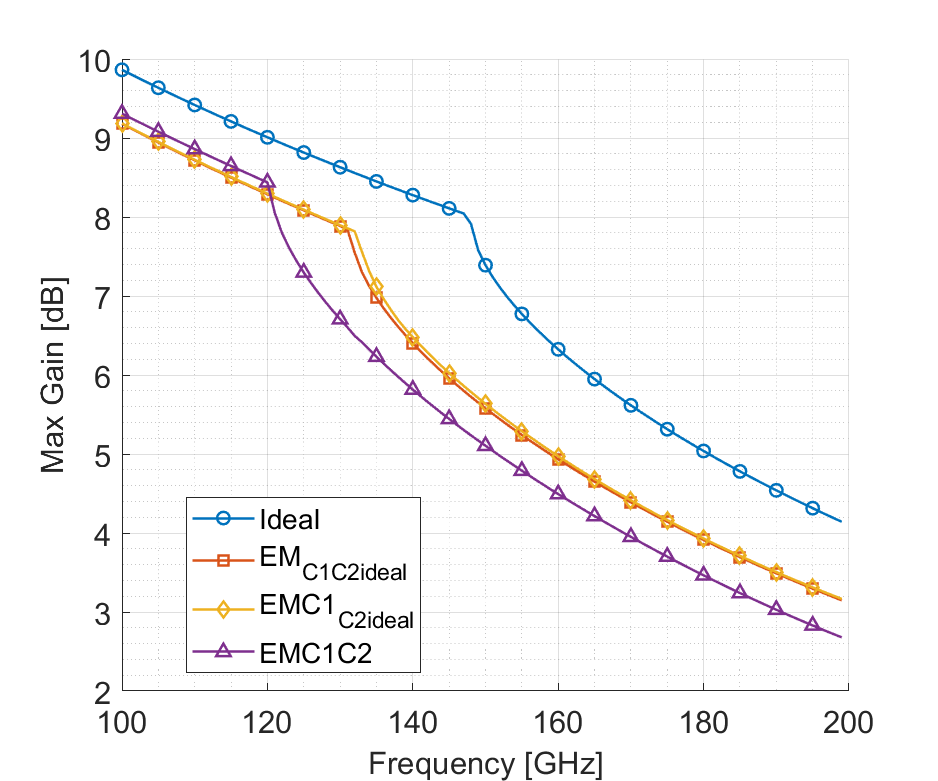
\includegraphics[width=0.5\linewidth]{Design_figures/Measurements/FirstStage/FirstStage_Ideal_VS_differentEM_MaxGain_Comparativo.png}
    \caption{Comparison of the MaxGain during the core design, in the following order: ideal; EM simulated core with ideal $C_1$ and $C_2$; EM simulated core with EM-simulated $C_1$ and ideal $C_2$; and EM-simulated core with EM simulated $C_1$ and $C_2$.}
    \label{fig:FirstStage_Ideal_VS_differentEM_MaxGain_Comparativo}
\end{figure}

\paragraph{Main parameters} In Figure \ref{fig:FirstStage_Ideal_VS_differentEM_MaxGain_Comparativo} is shown the MaxGain result in four different situations, as indicated in the figure itself.
The MaxGain line achieved with the core layout and  ideal C1 overlaps with the line of that obtained with the EM C1 within the layout, indicating that changes in the value of C1 does not affect the MaxGain. This is consistent with what is observed in Figure  \ref{fig:FirstStageSchematicMaxgainSweepC1}.\\
The deviation between the layout with EM simulated C1 and the full core with EM simulated C2 is obtained with the implementation of the transmission line paths at the inputs.\\
From the ideal topology in blue to the full EM simulated core in violet, a gain reduction of \SI{0.5}{\decibel} and \SI{1.5}{\decibel} over the frequency range can be noted.\\
The amplitude and phase imbalances are shown in Figure \ref{fig:FirstStage_Ideal_VS_differentEM_AmplitudeImbalance_Comparativo} and \ref{fig:FirstStage_Ideal_VS_differentEM_PhaseImbalance_Comparativo} respectively. 
\begin{figure}[H]
    \centering
    \begin{subfigure}{0.48\textwidth}
        \centering
        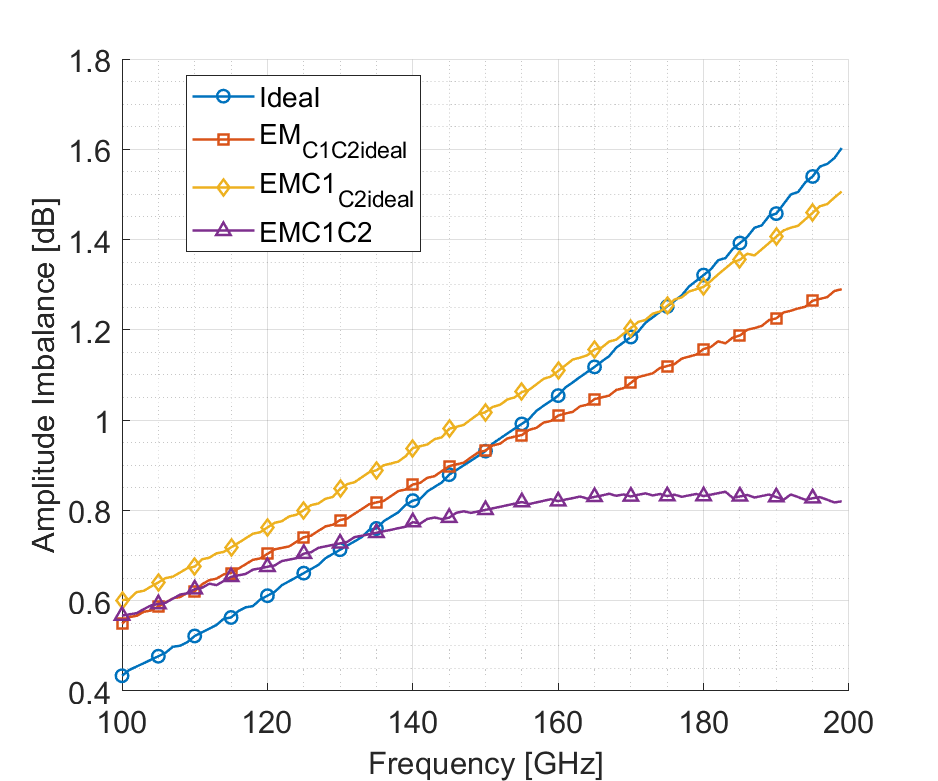
\includegraphics[width=\linewidth]{Design_figures/Measurements/FirstStage/FirstStage_Ideal_VS_differentEM_AmplitudeImbalance_Comparativo.png}
        \caption{}
        \label{fig:FirstStage_Ideal_VS_differentEM_AmplitudeImbalance_Comparativo}
    \end{subfigure}
    \hfill
    \begin{subfigure}{0.48\textwidth}
        \centering
        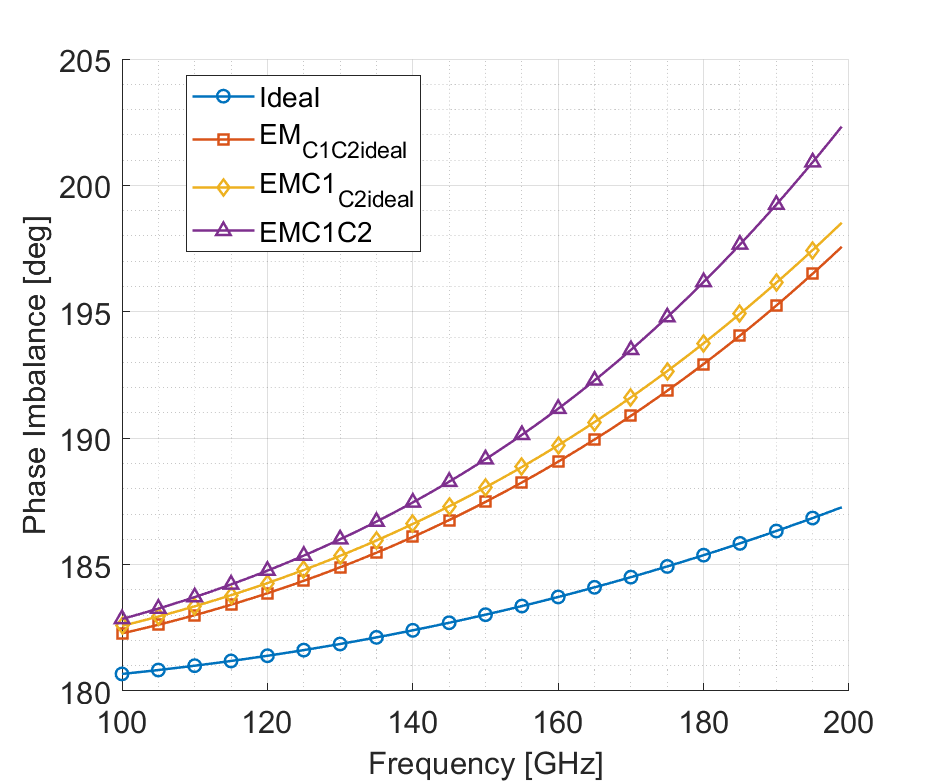
\includegraphics[width=\linewidth]{Design_figures/Measurements/FirstStage/FirstStage_Ideal_VS_differentEM_PhaseImbalance_Comparativo.png}
        \caption{}
        \label{fig:FirstStage_Ideal_VS_differentEM_PhaseImbalance_Comparativo}
    \end{subfigure}

    \caption{Simulated results and comparison of (a) amplitude imbalance and (b) phase imbalance during the core design, in the following order: ideal; EM simulated core with ideal $C_1$ and $C_2$; EM simulated core with EM simulated $C_1$ and ideal $C_2$; and EM simulated core with EM simulated $C_1$ and $C_2$.}
\end{figure}

From the amplitude imbalance it is possible to note a mild improvement when moving from the ideal core to its EM simulation with EM simulated C1 and ideal C2. Subsequently, with the transmission line connected and C2 EM simulated, the improvement becomes significant: at least 0.7 dB on the amplitude imbalance at 180GHz.

A first approximation analysis was performed to evaluate the cause of such significant change on the  parameters. Placing inductors in the ideal schematic to roughly emulate the transmission lines losses could explain the gain reduction. Furthermore, they do not explain the balance variation if the symmetry assumption is still considered to be valid.

The discrepancy on the balance results has to be associated with the implementation of the transmission line and the C2 capacitor in the layout.
Regarding this matter, a quick look at the performances of the differential second stage in Figure \ref{fig:SecondStageLayout} can be taken into account. Its results demonstrate that the symmetry of the circuit is preserved after the addition of the transmission lines bringing to the conclusion that the C2 capacitor is responsible of the deviations, particularly, the parasitics that it is creating with the surrounding elements and the fact that its capacitance is reducing after \SI{150}{\giga\hertz}, as shown in Appendix \ref{sec:Appendix}, Figure \ref{fig:Layout_ShuntCapacitor}. 

More precise observations can be given by analyzing the differential gain of the three port. Figure~\ref{fig:ComparisonIdealBalun_AllY} displays the Y-parameters behavior of the ideal balun presented in Figure~\ref{fig:SchematicfirstStage}.
\begin{figure}[hbt!]
    \centering
    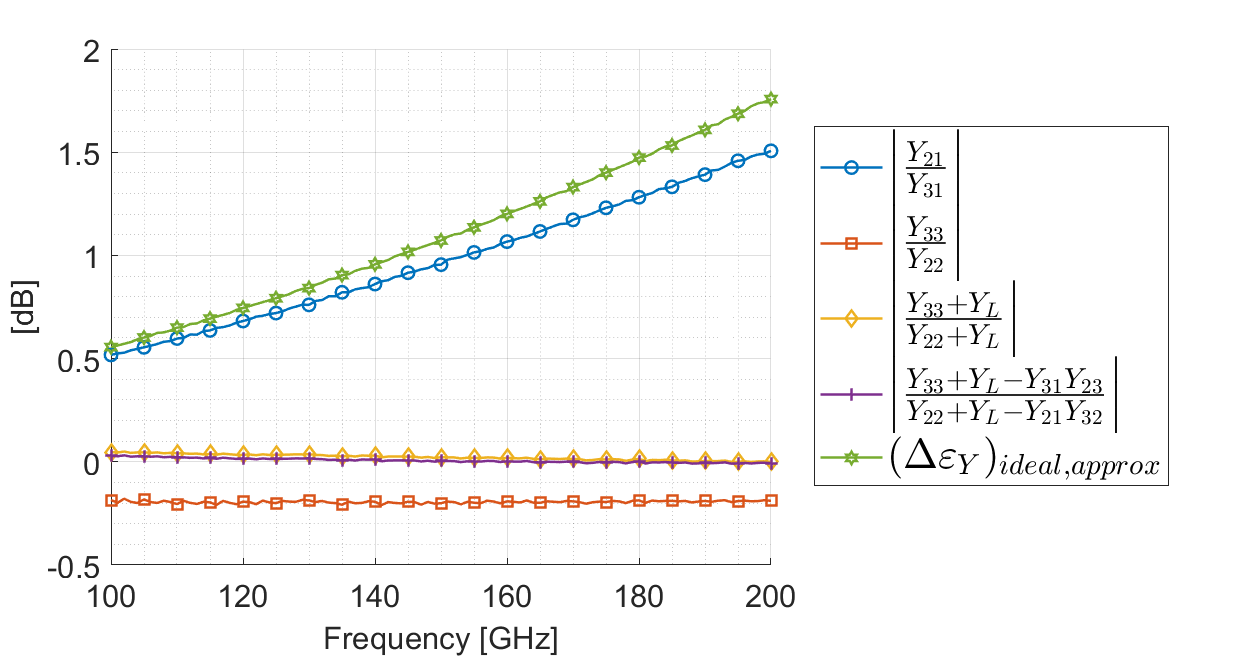
\includegraphics[width=0.76\linewidth]{Design_figures/Layout/ComparisonMeasurements/DiffBalun1Z_ExtractPar_C1C2fixed_S_MaxGain_ComparisonIdealBalun_AllY.png}
    \caption{Simulation of the Y parameters contributing to the amplitude imbalance of the first ideal stage.}
    \label{fig:ComparisonIdealBalun_AllY}
\end{figure}\\
As a first approximation, the second term can be evaluated by neglecting the $Y_{31}Y_{23}$ and $Y_{21}Y_{32}$ terms.

The ratio $|Y_{21}/Y_{31}|_{\mathrm{dB}}$ ranges from \SI{0.5}{\decibel} to \SI{1.5}{\decibel}, meaning that $Y_{21}$ is greater than $Y_{31}$ over the whole frequency range.
The ratio $|Y_{33}/Y_{22}|_{\mathrm{dB}}$ is constant and approximately \SI{-0.2}{\decibel}, meaning that $Y_{22}$ is slightly greater than $Y_{33}$.\\
When the load admittance is included in the second term, the ratio becomes approximately \SI{0}{\decibel}, meaning that $Y_L$ is greater than both $Y_{33}$ and $Y_{22}$.

Finally, the trend of the approximated amplitude imbalance in the ideal topology, $(\Delta \varepsilon)$, evaluated with~\eqref{eq:DiffGainBalanceYportsApprox}, shows that its trend is close to $|Y_{21}/Y_{31}|_{\mathrm{dB}}$.

Figure~\ref{fig:ComparisonEmBalun_AllY} shows the Y-parameters behavior of the EM simulated core, previously presented in the plots as (EMC1C2) and whose 3D circuit layout is shown in Figure~\ref{fig:3Dlayoutview}.
\begin{figure}[hbt!]
    \centering
    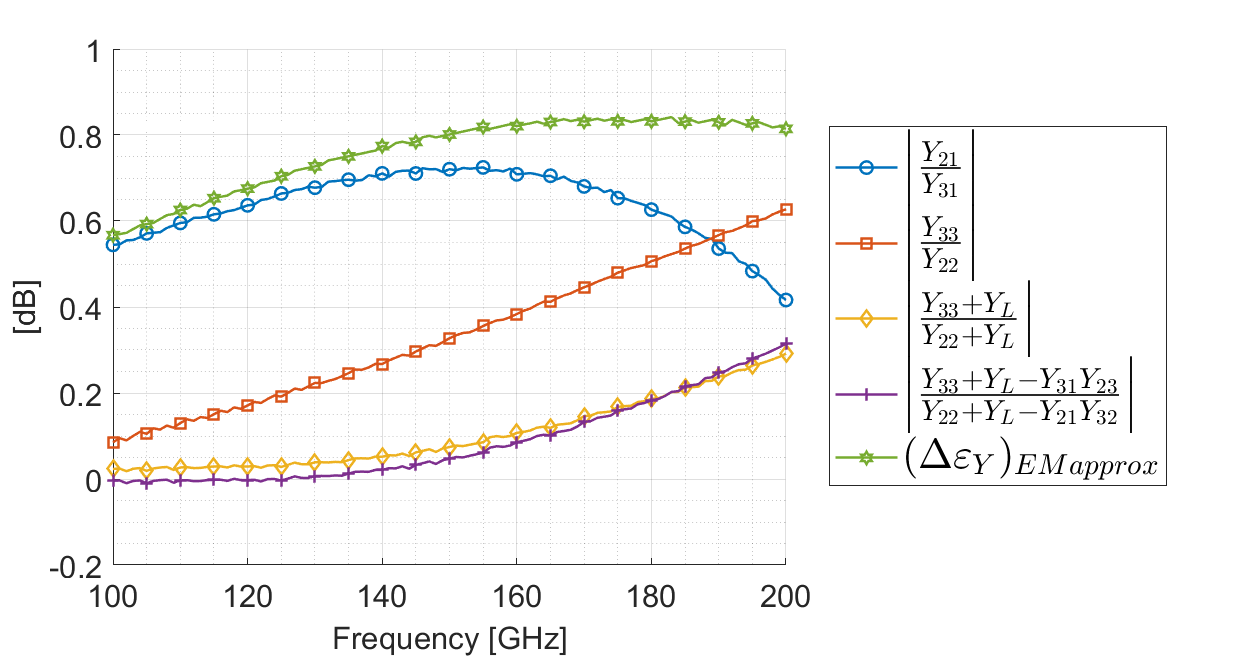
\includegraphics[width=0.75\linewidth]{Design_figures/Layout/ComparisonMeasurements/DiffBalun1Z_ExtractPar_C1C2fixed_S_MaxGain_ComparisonEmBalun_AllY.png}
    \caption{Simulation of the Y parameters contributing to the amplitude imbalance of the first stage with an EM simulated core.}
    \label{fig:ComparisonEmBalun_AllY}
\end{figure}\\
While keeping the approximations on the $Y_{31}Y_{23}$ and $Y_{21}Y_{32}$ terms, important differences can be observed. First, the trend of $|Y_{21}/Y_{31}|_{\mathrm{dB}}$ is no longer monotonic, with $Y_{31}$ that becomes greater than $Y_{21}$ above \SI{150}{\giga\hertz}.
Secondly, the ratio $|Y_{33}/Y_{22}|_{\mathrm{dB}}$ increases with frequency. These behaviors can be related to the reduction of the capacitance value of $C_2$ , which in turns  changes the CB input and output impedances as the frequency increases, especially above \SI{150}{\giga\hertz}.

At the output, this leads to an increase in $Y_{33}$. In fact, above \SI{150}{\giga\hertz}, the second term starts to increase, showing that the numerator is no longer dominated by $Y_L$, but by $Y_{33}$. As a result, the magnitude of the second term increases.

In Appendix~\ref{sec:Appendix}, Figure~\ref{fig:DiffAmpS_vsY} shows the differences and the discrepancies between the amplitude imbalances defined by the three equations \eqref{eq:DiffGainBalanceSports}, \eqref{eq:DiffGainBalanceYportsApprox}, and \eqref{eq:DiffGainBalanceYportsComplete}.

\paragraph{Stability} Since the balun is a three port network but the stability parameters are defined for two-port networks only, the analysis was split in two. Figures \ref{fig:EMDiffBalun2_ExtractPar_LongTM2_S_MaxGain_S21_StabilityParameters},  \ref{fig:EMDiffBalun2_ExtractPar_LongTM2_S_MaxGain_S21_SourceStability} and \ref{fig:EMDiffBalun2_ExtractPar_LongTM2_S_MaxGain_S21_LoadStability} refer to simulations with port 3 terminated at an ideal \SI{50}{\ohm} load, while Figures \ref{fig:EMDiffBalun2_ExtractPar_LongTM2_S_MaxGain_S31_StabilityParameters},  \ref{fig:EMDiffBalun2_ExtractPar_LongTM2_S_MaxGain_S31_SourceStability} and \ref{fig:EMDiffBalun2_ExtractPar_LongTM2_S_MaxGain_S31_LoadStability} refer to simulations with port 2 terminated at an ideal \SI{50}{\ohm} load.

\begin{figure}[hbt!]
    \centering
    \begin{subfigure}{0.49\textwidth}
        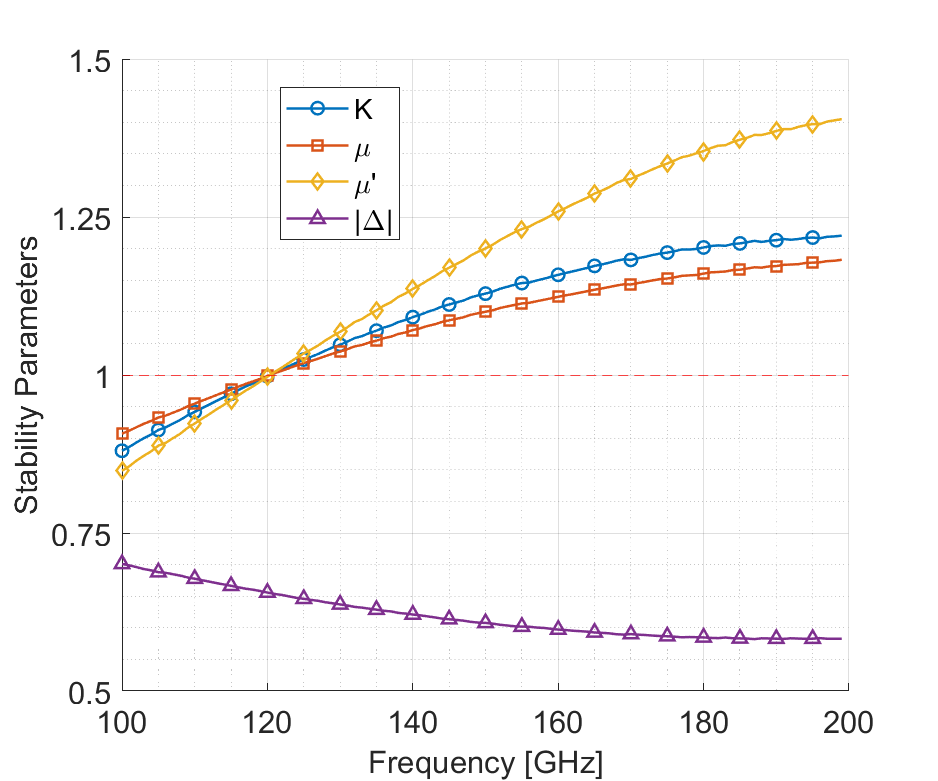
\includegraphics[width=\linewidth]{Design_figures/Measurements/FirstStage/EMDiffBalun2_ExtractPar_LongTM2_S_MaxGain_S21_StabilityParameters.png}
        \caption{}
        \label{fig:EMDiffBalun2_ExtractPar_LongTM2_S_MaxGain_S21_StabilityParameters}
    \end{subfigure}
    \hfill
    \begin{subfigure}{0.49\textwidth}
        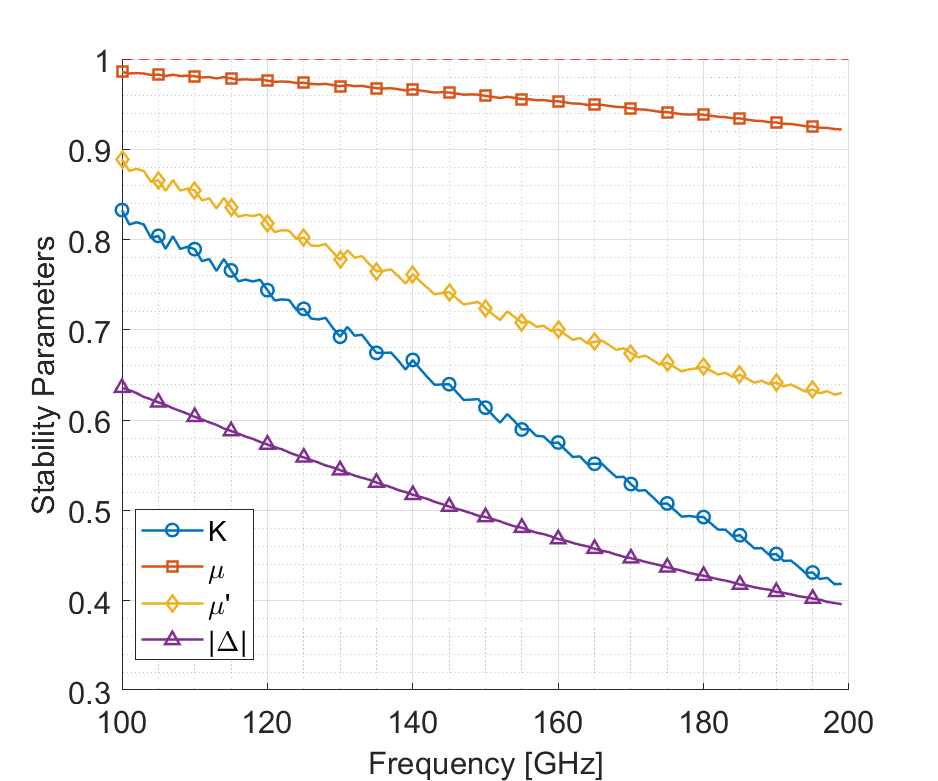
\includegraphics[width=\linewidth]{Design_figures/Measurements/FirstStage/EMDiffBalun2_ExtractPar_LongTM2_S_MaxGain_S31_StabilityParameters.png}
        \caption{}
        \label{fig:EMDiffBalun2_ExtractPar_LongTM2_S_MaxGain_S31_StabilityParameters}
    \end{subfigure}
    \caption{Simulated stability parameters of the single-input balanced-output differential amplifier layout (EMC1C2): (a) Port3 terminated with \SI{50}{\ohm} and output at Port2; (b) Port2 terminated with \SI{50}{\ohm} and output at Port3.}
    \label{fig:placeholder}
\end{figure}

Due to the fact that the stability factors modules are not greater than 1 in all the frequency range, a deeper study must be performed by analyzing the stability circles of the unilateral device so to know the instability regions and hence to avoid the impedances which cause oscillations.\\
The Smith Plots also include the necessary reflection coefficients: in Figure \ref{fig:EMDiffBalun2_ExtractPar_LongTM2_S_MaxGain_S21_SourceStability} and \ref{fig:EMDiffBalun2_ExtractPar_LongTM2_S_MaxGain_S31_SourceStability} is plotted the $S_{11}$ value, meanwhile in Figure  
\ref{fig:EMDiffBalun2_ExtractPar_LongTM2_S_MaxGain_S21_LoadStability} and
 and \ref{fig:EMDiffBalun2_ExtractPar_LongTM2_S_MaxGain_S31_LoadStability}  are plotted the respective $S_{22}$ values.

\begin{figure}[hbt!]
    \centering
    \begin{subfigure}{0.43\textwidth}
        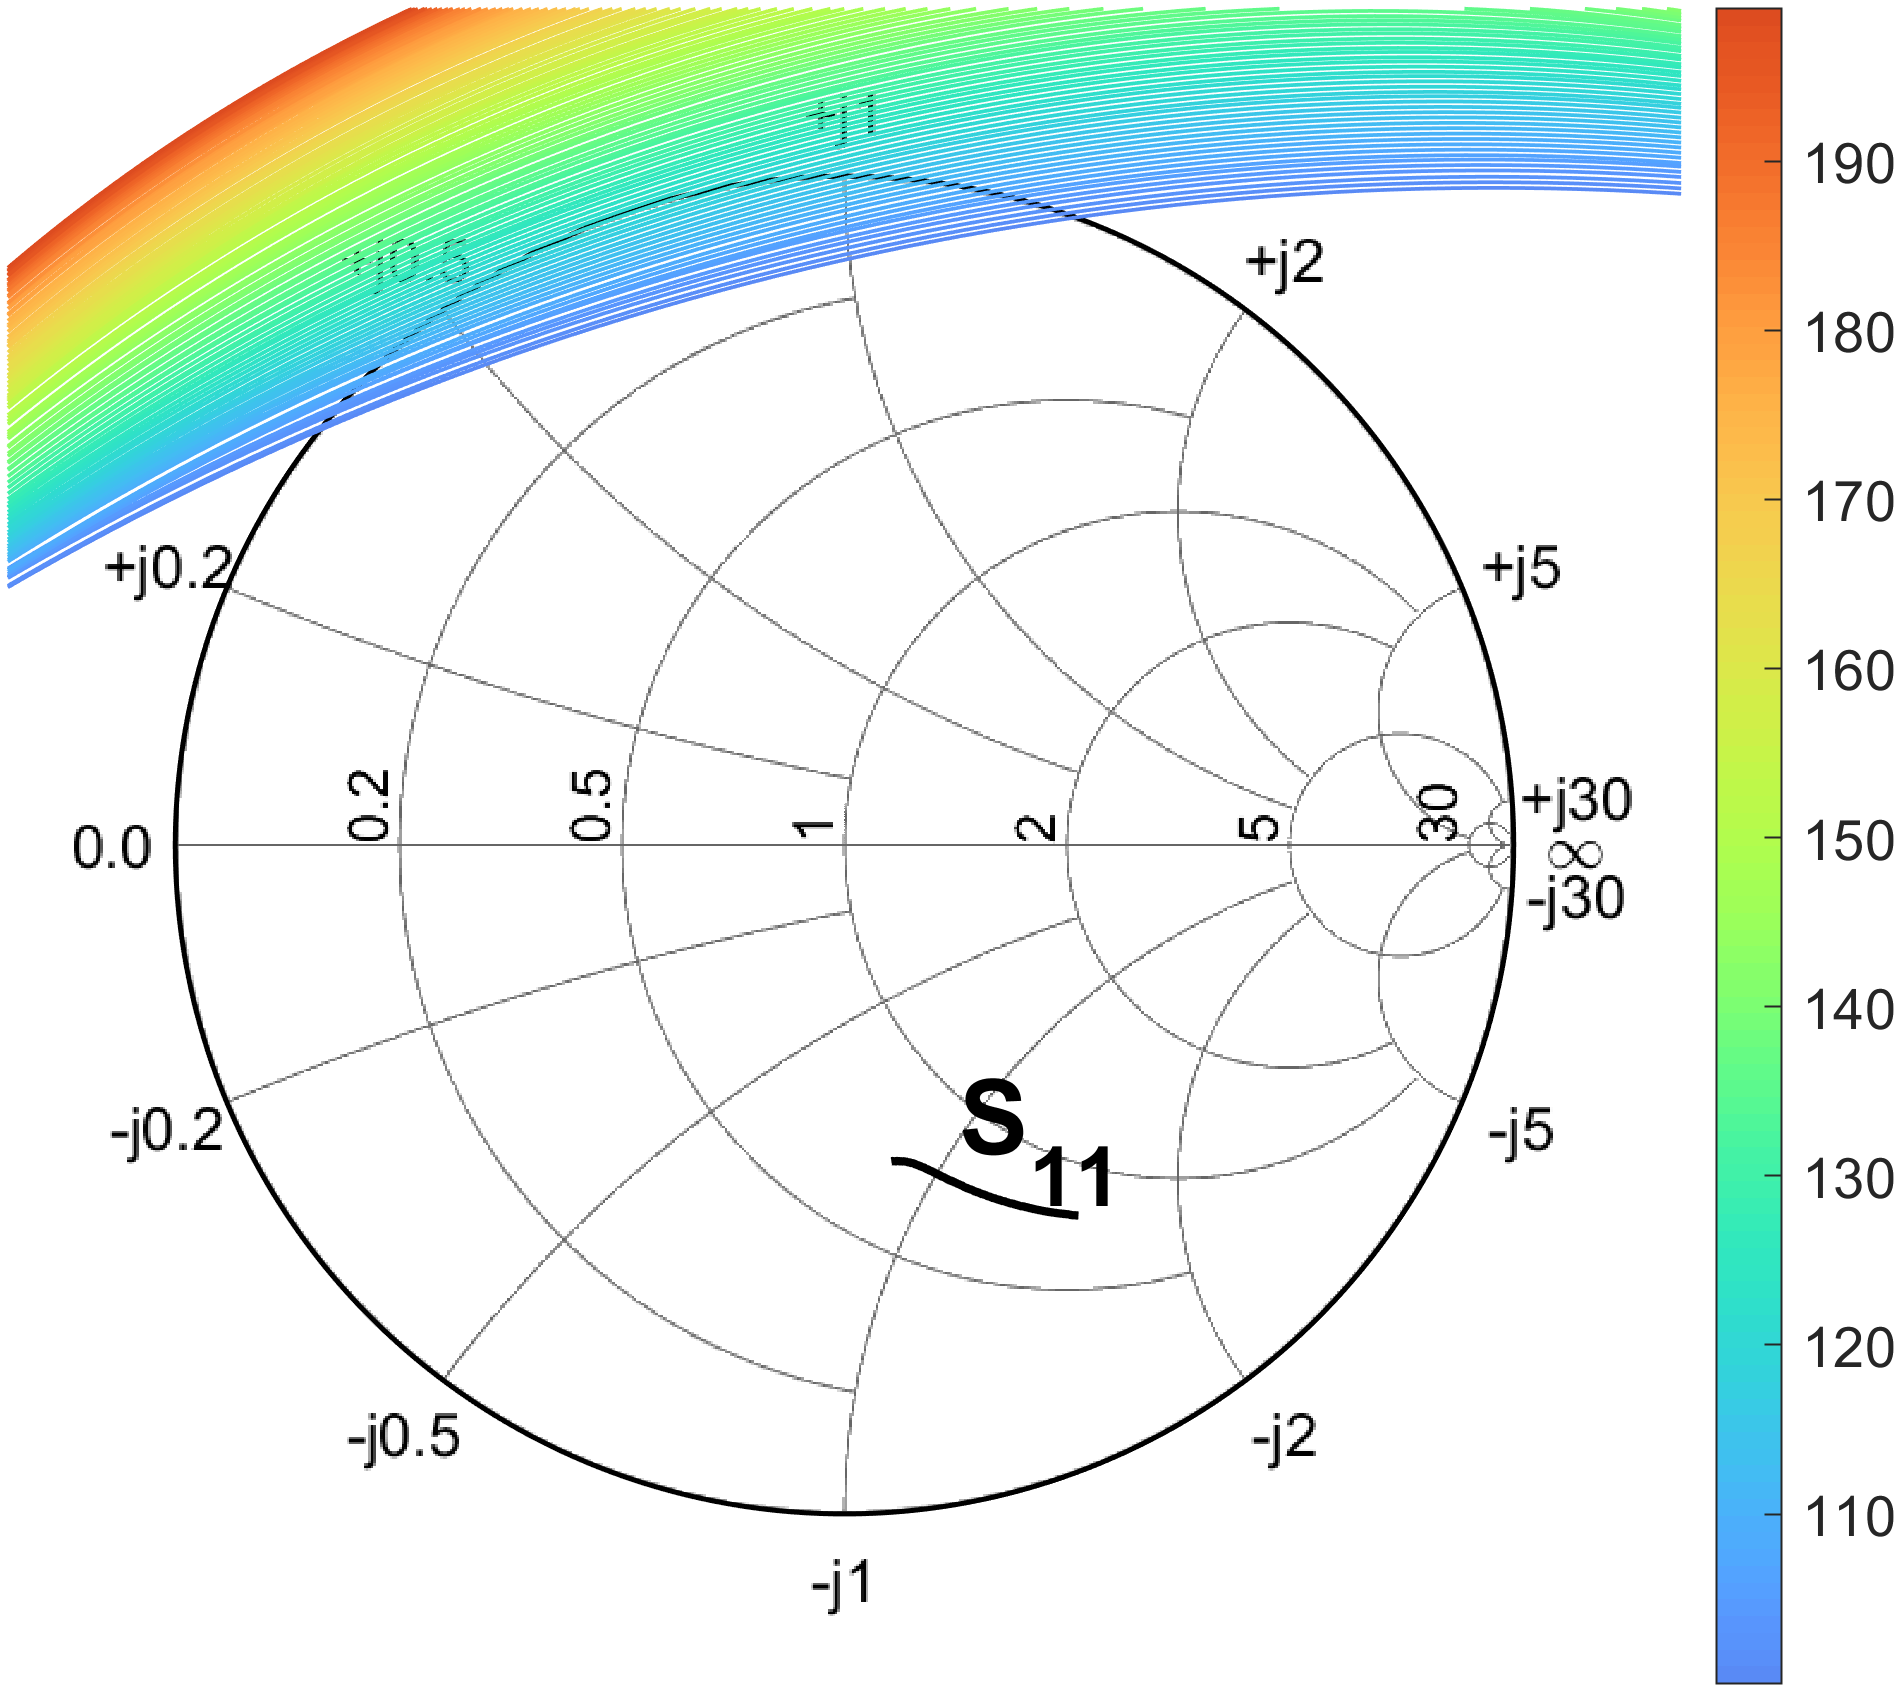
\includegraphics[width=0.95\linewidth]{Design_figures/Measurements/FirstStage/EMDiffBalun2_ExtractPar_LongTM2_S_MaxGain_S21_SourceStability.png}
        \caption{}
        \label{fig:EMDiffBalun2_ExtractPar_LongTM2_S_MaxGain_S21_SourceStability}
    \end{subfigure}
    \hfill
    \begin{subfigure}{0.43\textwidth}
        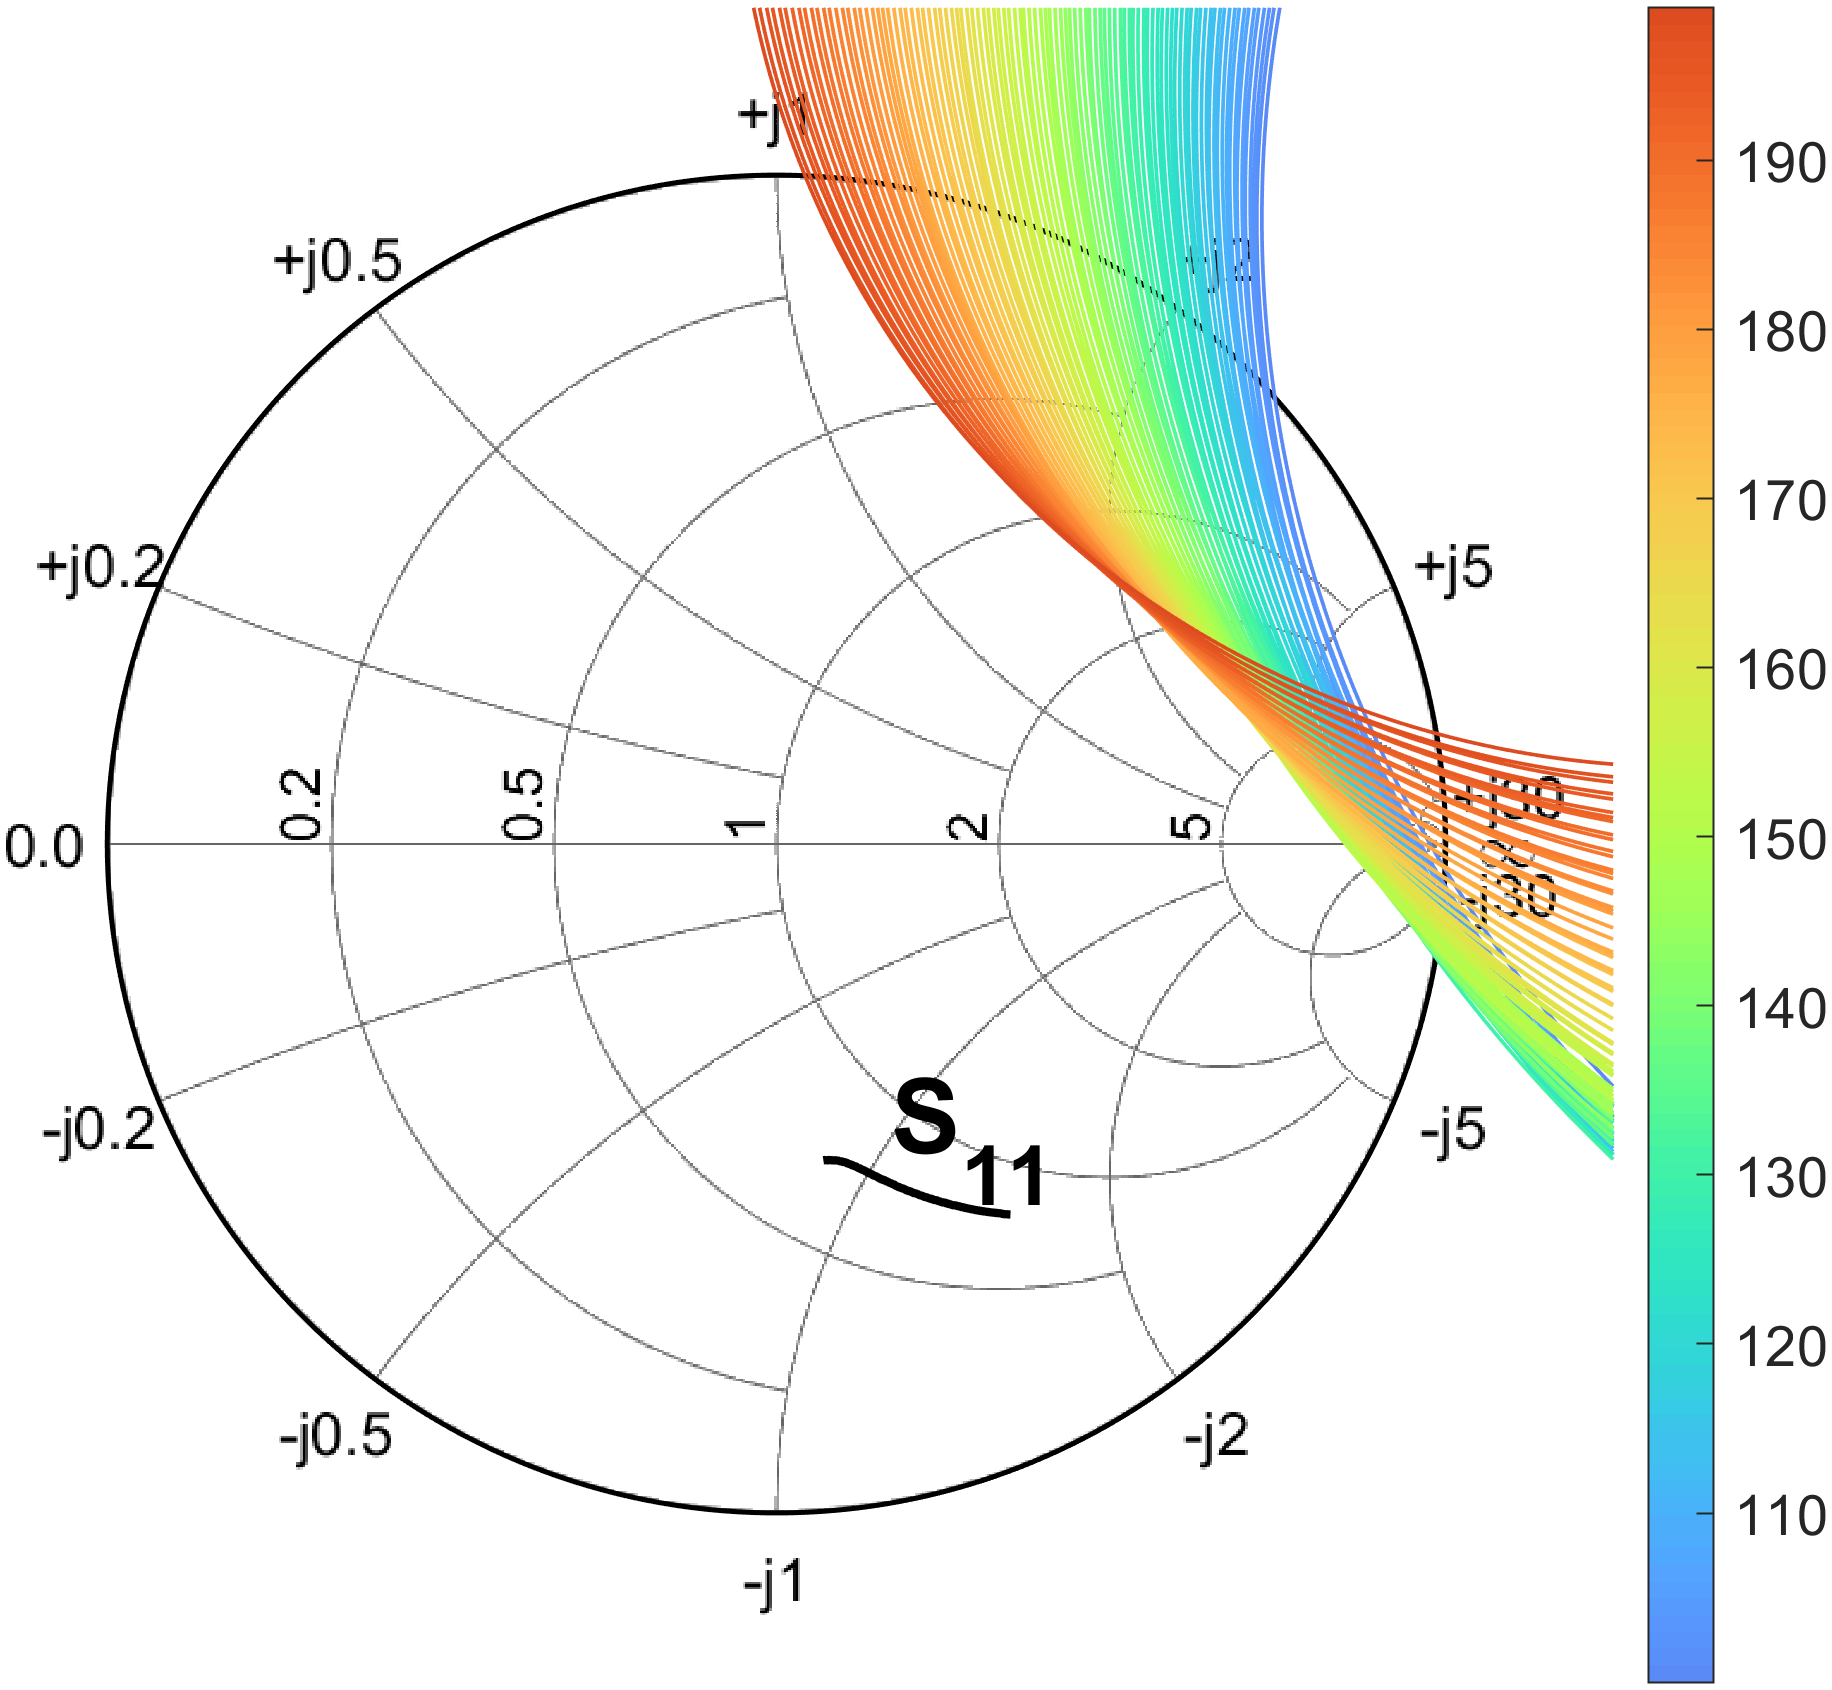
\includegraphics[width=0.95\linewidth]{Design_figures/Measurements/FirstStage/EMDiffBalun2_ExtractPar_LongTM2_S_MaxGain_S31_SourceStability.png}
        \caption{}
        \label{fig:EMDiffBalun2_ExtractPar_LongTM2_S_MaxGain_S31_SourceStability}
    \end{subfigure}
    \caption{Simulated source stability circles of the single-input balanced-output differential amplifier layout (EMC1C2):  (a) Port3 terminated with \SI{50}{\ohm} and output at Port2, (b) Port2 terminated with \SI{50}{\ohm} and output at Port3}
    \label{fig:placeholder}
\end{figure}
\begin{figure}[hbt!]
    \centering
    \begin{subfigure}{0.43\textwidth}
        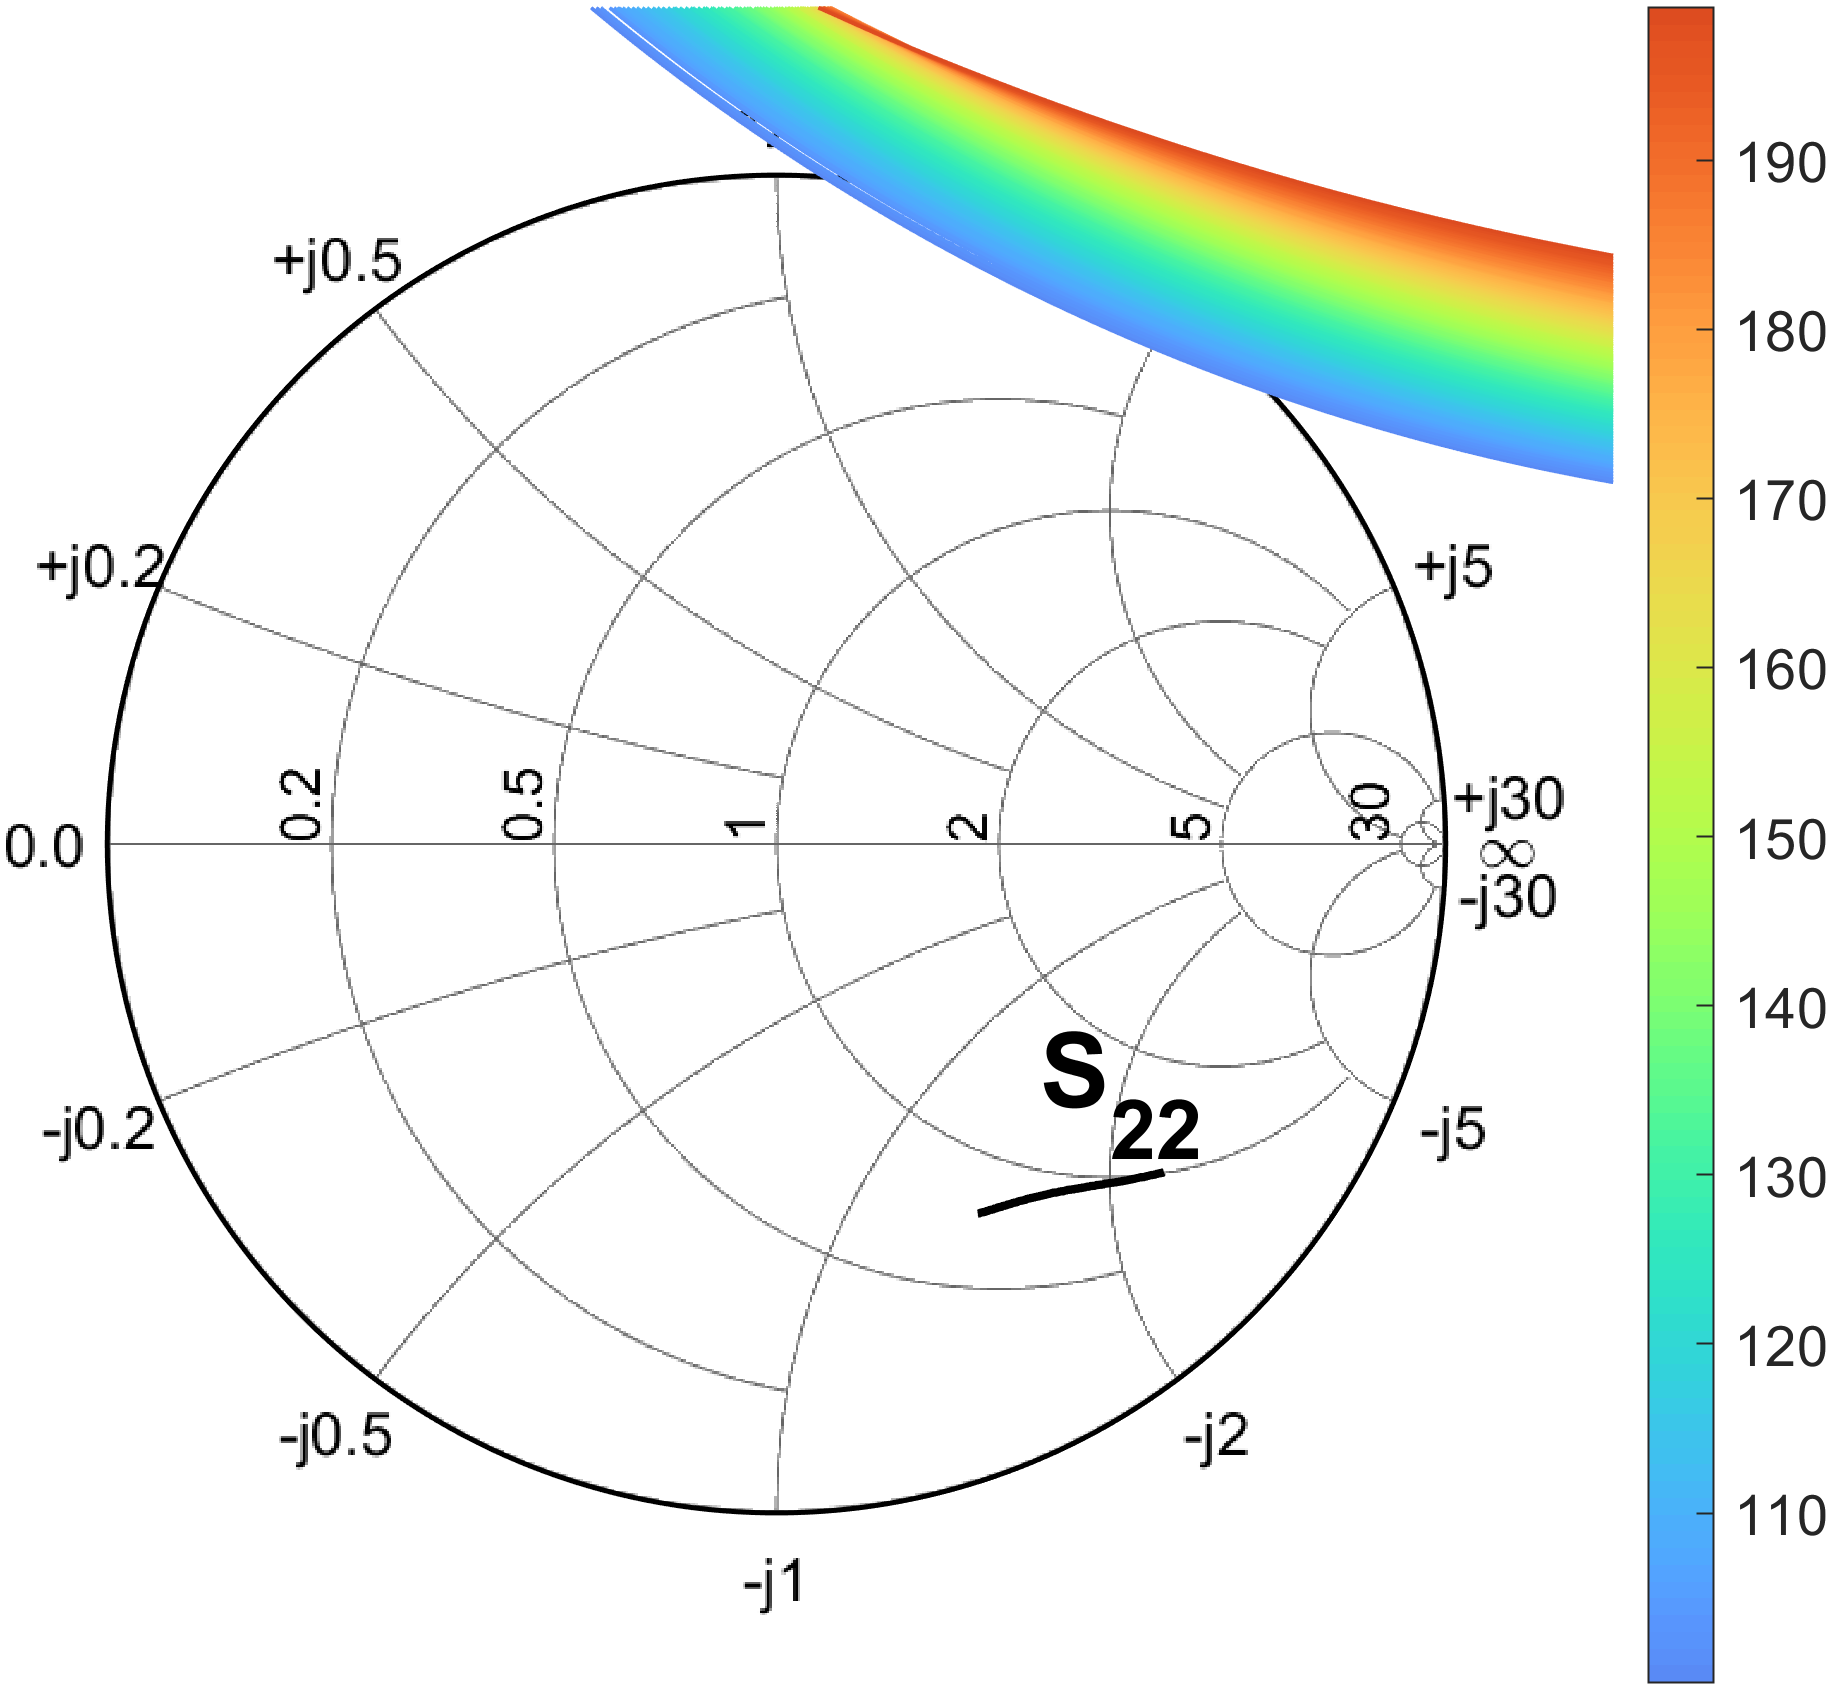
\includegraphics[width=0.95\linewidth]{Design_figures/Measurements/FirstStage/EMDiffBalun2_ExtractPar_LongTM2_S_MaxGain_S21_LoadStability.png}
        \caption{}
        \label{fig:EMDiffBalun2_ExtractPar_LongTM2_S_MaxGain_S21_LoadStability}
    \end{subfigure}
    \hfill
    \begin{subfigure}{0.43\textwidth}
        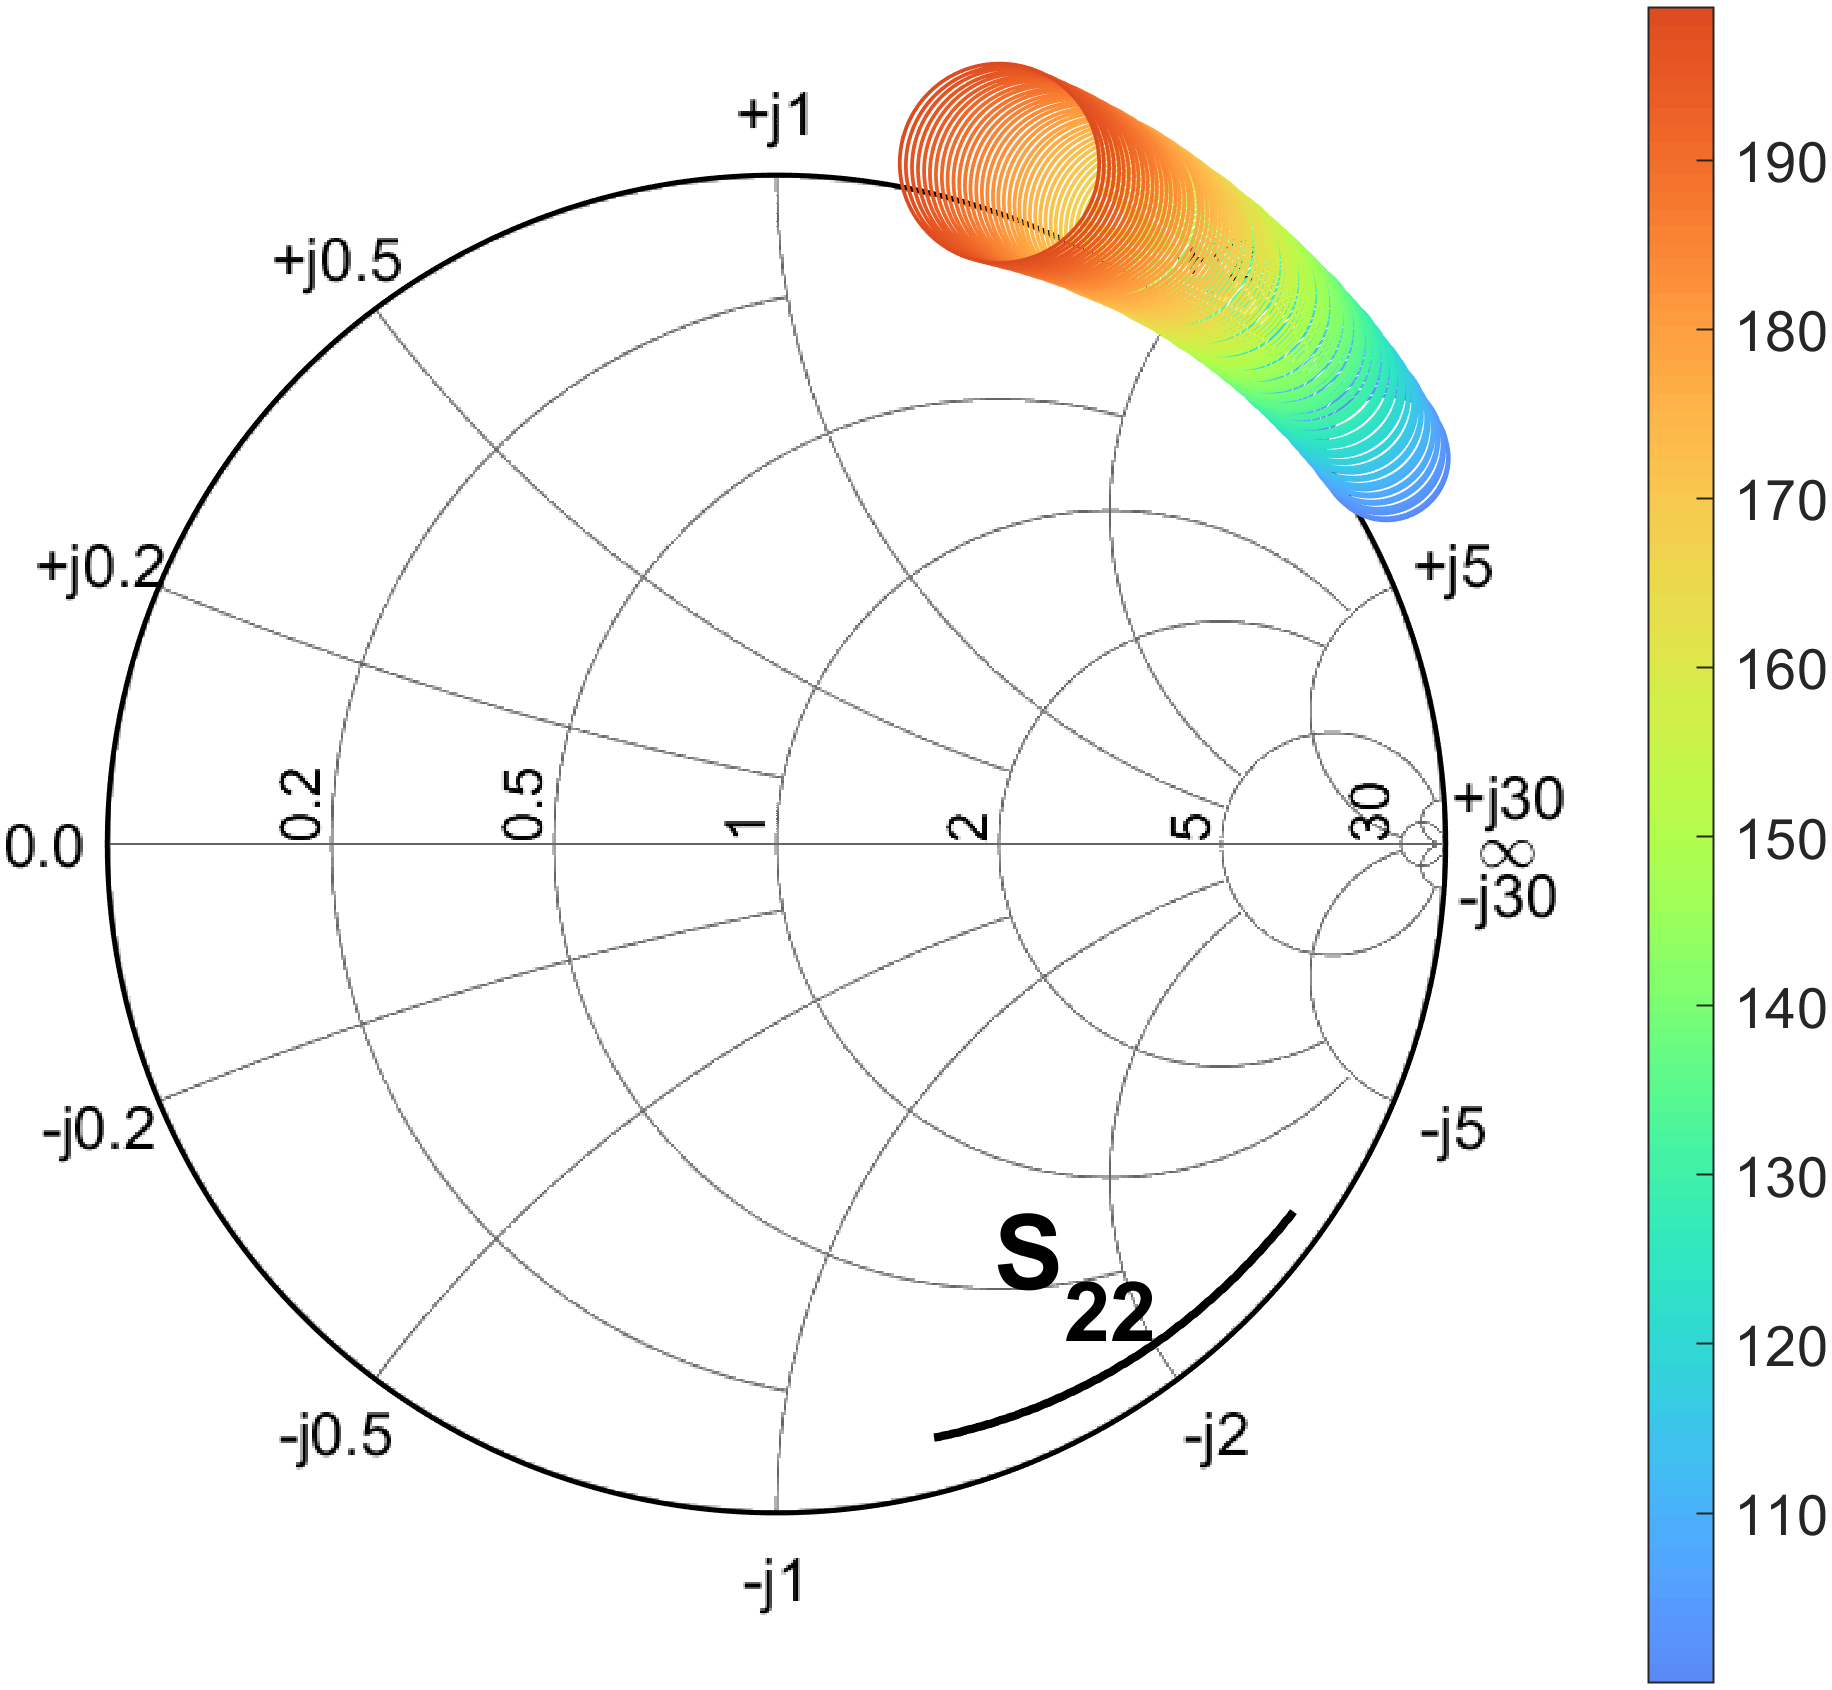
\includegraphics[width=0.95\linewidth]{Design_figures/Measurements/FirstStage/EMDiffBalun2_ExtractPar_LongTM2_S_MaxGain_S31_LoadStability.png}
        \caption{}
        \label{fig:EMDiffBalun2_ExtractPar_LongTM2_S_MaxGain_S31_LoadStability}
    \end{subfigure}
    \caption{Simulated load stability circles of the single-input balanced-output differential amplifier layout (EMC1C2): (a) Port 3 terminated with \SI{50}{\ohm} and output at Port2; (b) Port2 terminated with \SI{50}{\ohm} and output at Port3.}
    \label{fig:placeholder}
\end{figure}

Since the reflection parameters are inside the Smith chart, their magnitudes are lower than unity and therefore the stable region is the one containing the center of the Smith chart\cite{Microwave Transistor Amplifiers Analysis and Design}.
Starting from the case with port three terminated to an ideal load, it is possible to note that the source stability circles in Figure \ref{fig:EMDiffBalun2_ExtractPar_LongTM2_S_MaxGain_S21_SourceStability} includes the center of the Smith chart. This results in inconditional stability in almost the entire plot region, except for a portion when operating from \SIrange{100}{120}{\giga\hertz}. The load stability circle in Figure \ref{fig:EMDiffBalun2_ExtractPar_LongTM2_S_MaxGain_S21_LoadStability} does not include the center of the Smith chart, meaning that the port operates in conditional stability in almost the entire region except for 
the one inside the intersection with the circle $\Gamma_S=S_{22}$ at the same frequencies as the source stability.

In the case with port two terminated to an ideal load, the results are interpreted in the same way. The only difference is that the source stability circle in Figure \ref{fig:EMDiffBalun2_ExtractPar_LongTM2_S_MaxGain_S31_SourceStability} includes a greater instability region, especially beyond \SI{120}{\giga\hertz}, while the load stability circle in Figure \ref{fig:EMDiffBalun2_ExtractPar_LongTM2_S_MaxGain_S31_LoadStability} shows almost all the point in the Smith chart to be stable.
%%%%
\subsubsection{Second Stage}
The core layout of the second stage is identical to what is shown in Figure \ref{fig:Corelayoutofthedifferentialstages} and \ref{fig:FigureSimulationCoreLayoutC1EMC2ideal}. The simulated schematic is shown in Figure \ref{fig:SecondStageLayout}.
\begin{figure}[hbt!]
    \centering
        \begin{overpic}[width=0.85\linewidth]{Design_figures/Schematics/SecondStageLayout.png}
        \put(43,22.5){\footnotesize Q8}
        \put(49.5,22.5){\footnotesize Q7}
        \put(51,40){\footnotesize Q5}
        \put(51,9){\footnotesize Q6}
        \put(26,29,5){\footnotesize $\dfrac{C1}{2}$}
        \put(26,19){\footnotesize $\dfrac{C1}{2}$}
        \put(42,40){\footnotesize R5}
        \put(42,8.5){\footnotesize R6}
        \put(17.5,32.25){\footnotesize 2*R7}
        \put(17.5,16.5){\footnotesize 2*R7}
        \put(31,25.5){\footnotesize R8}
        
    \end{overpic}
    \caption{Simulation of the the double input-balanced output differential amplifier schematic with EM core}
    \label{fig:SecondStageLayout}
\end{figure}
%
\paragraph{Main parameters} The amplitude imbalance and phase imbalance were simulated with an ideal differential input and the result showns in Figure \ref{fig:EM_DiffAmplifier1_ExtractPar_LongInputTM2_S_MaxGain_AmplitudePhaseImbalance} indicate that a good quality on the symmetry of the core is achieved. The amplitude imbalance on Figure \ref{fig:EM_DiffAmplifier1_ExtractPar_LongInputTM2_S_MaxGain_AmplitudePhaseImbalance} is, in fact, so low and negligible that the MATLAB plot shows mathematical errors. To try to match the results with the ADS simulations, a linear interpolation on some values is performed. The same behavior can be associated with the phase imbalance, but a quick zoom out of the axis gives a better result.
%
\begin{figure}[hbt!]
    \centering
    \begin{subfigure}{0.48\textwidth}
    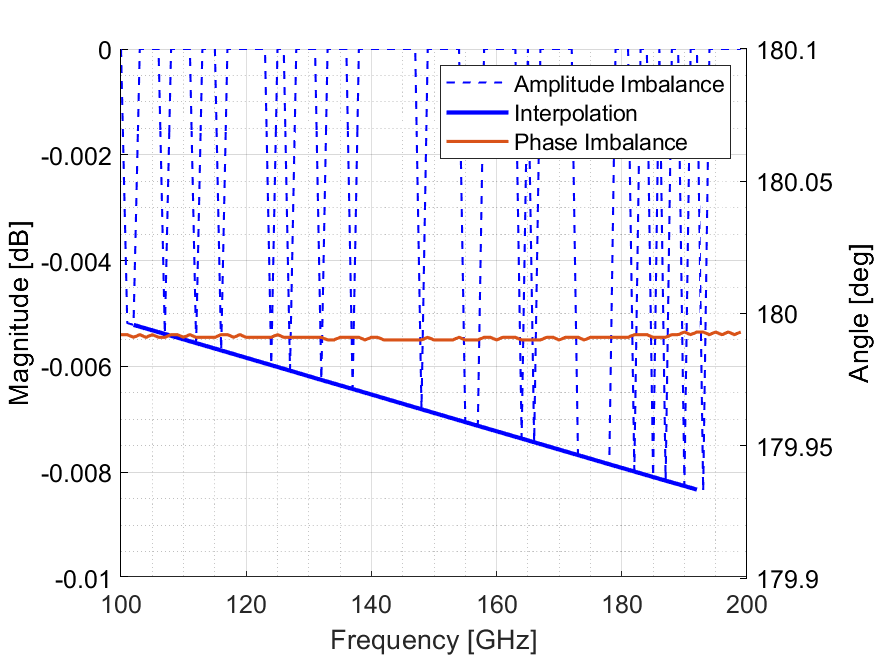
\includegraphics[width=\linewidth]{Design_figures/Measurements/SecondStage/EM_DiffAmplifier1_ExtractPar_LongInputTM2_S_MaxGain_AmplitudePhaseImbalance.png}
    \caption{}
    \label{fig:EM_DiffAmplifier1_ExtractPar_LongInputTM2_S_MaxGain_AmplitudePhaseImbalance}
    \end{subfigure}
    \hfill
    \begin{subfigure}{0.48\textwidth}
         \centering
        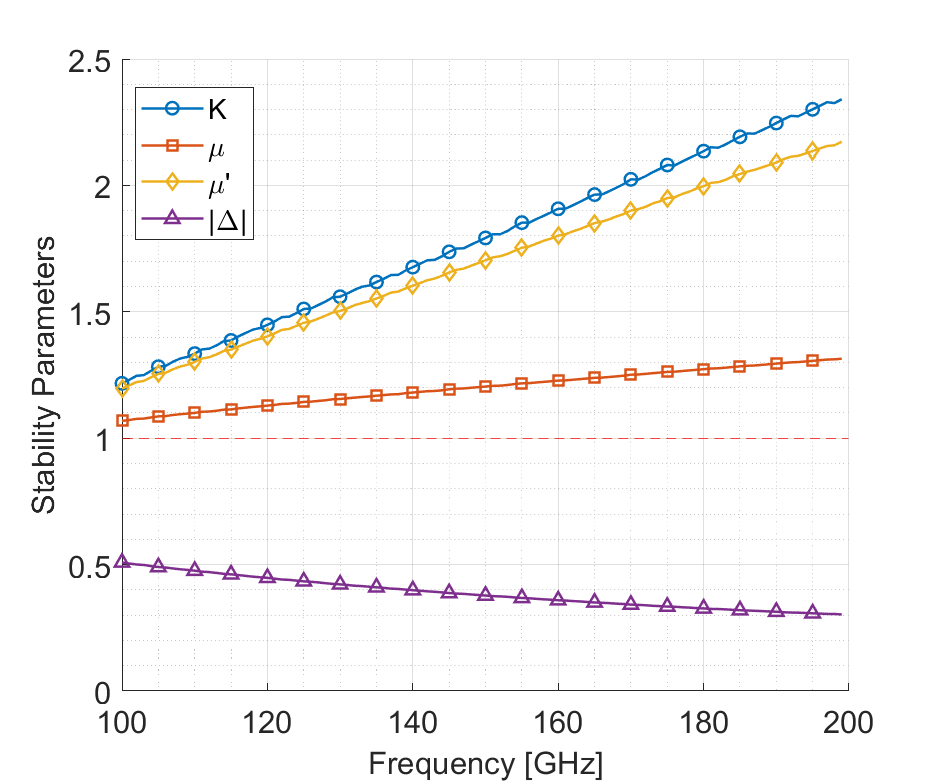
\includegraphics[width=\linewidth]{Design_figures/Measurements/SecondStage/EM_DiffAmplifier1_ExtractPar_LongInputTM2_S_MaxGain_S21_StabilityParameters.png}
    \caption{}\label{fig:EM_DiffAmplifier1_ExtractPar_LongInputTM2_S_MaxGain_S21_StabilityParameters}
    \end{subfigure}
    \caption{Simulated results of the (a) amplitude and phase imbalances and (b) stability parameters of the double input-balanced output differential amplifier layout}
\end{figure}
%
\mbox{}\\ 
\mbox{}\\
\paragraph{Stability} The stability analysis is performed as in the first stage but this time the stability parameters at the output ports are symmetrical, because of this, only the simulation with port 3 terminated at ideal 50 ohm are reported. Figure \ref{fig:EM_DiffAmplifier1_ExtractPar_LongInputTM2_S_MaxGain_S21_StabilityParameters} shown the stability factors, Figure \ref{fig:EM_DiffAmplifier1_ExtractPar_LongInputTM2_S_MaxGain_SourceStability} stability circles at input and \ref{fig:EM_DiffAmplifier1_ExtractPar_LongInputTM2_S_MaxGain_LoadStability} stability circles at load, simulated between \SI{100}{\giga\hertz} and \SI{200}{\giga\hertz} .
%
\begin{figure}[hbt!]
    \centering
    \begin{subfigure}{0.43\textwidth}
        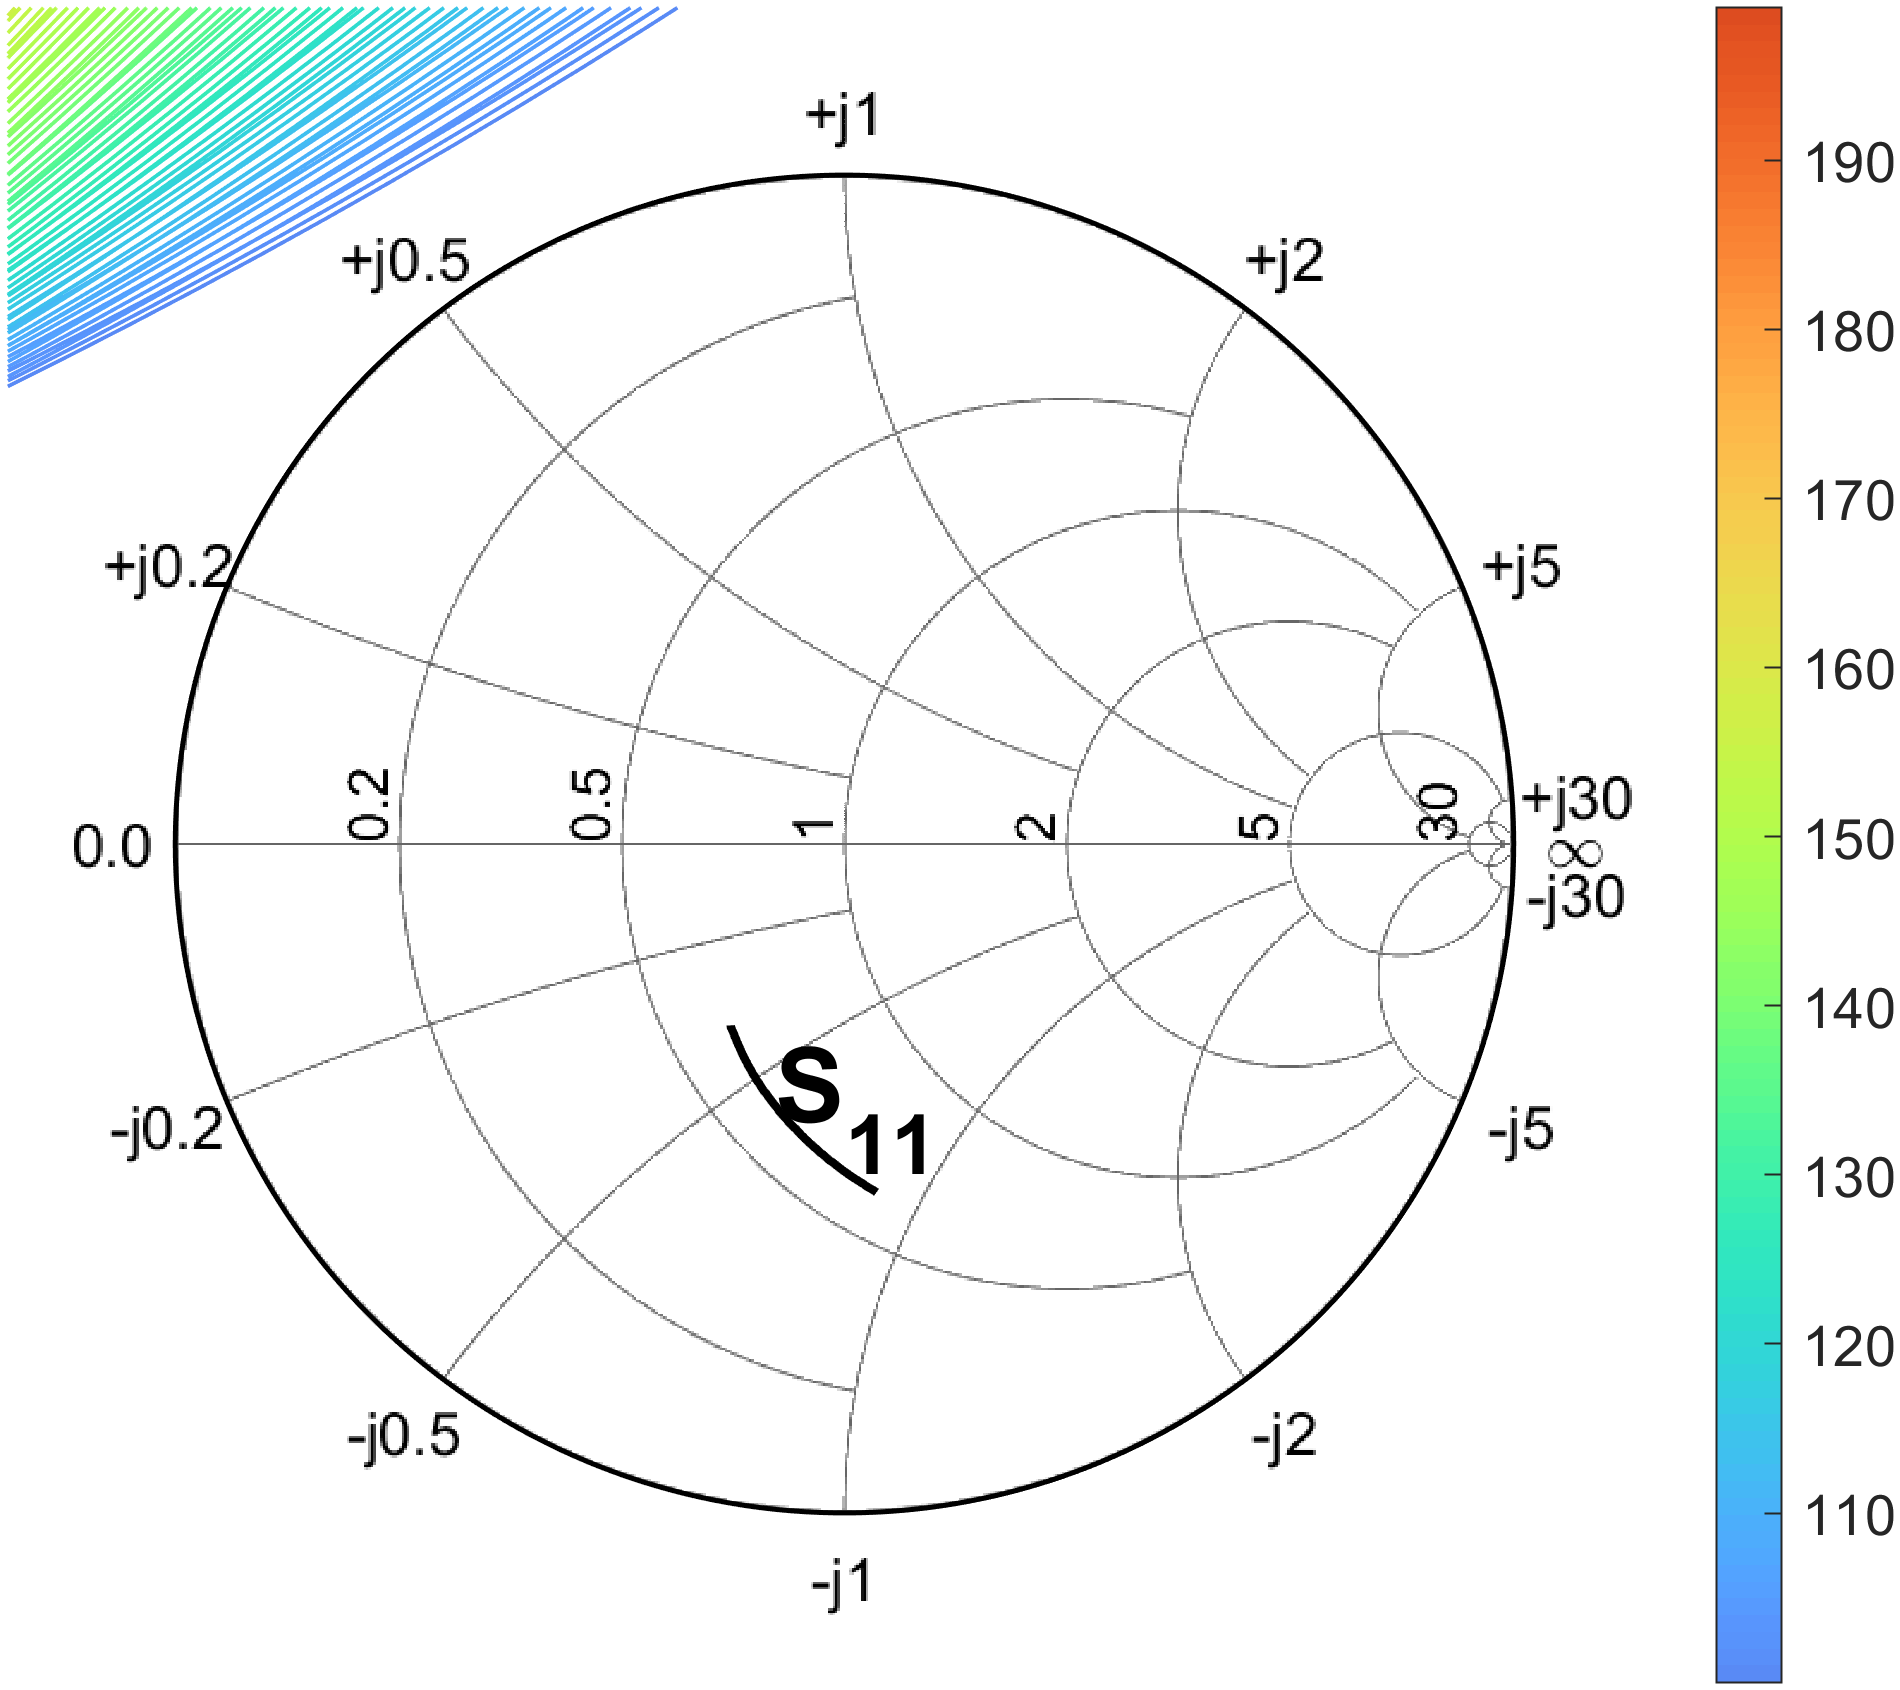
\includegraphics[width=0.95\linewidth]{Design_figures/Measurements/SecondStage/EM_DiffAmplifier1_ExtractPar_LongInputTM2_S_MaxGain_S21_SourceStability.png}
        \caption{}
        \label{fig:EM_DiffAmplifier1_ExtractPar_LongInputTM2_S_MaxGain_SourceStability}
    \end{subfigure}
    \hfill
    \begin{subfigure}{0.43\textwidth}
        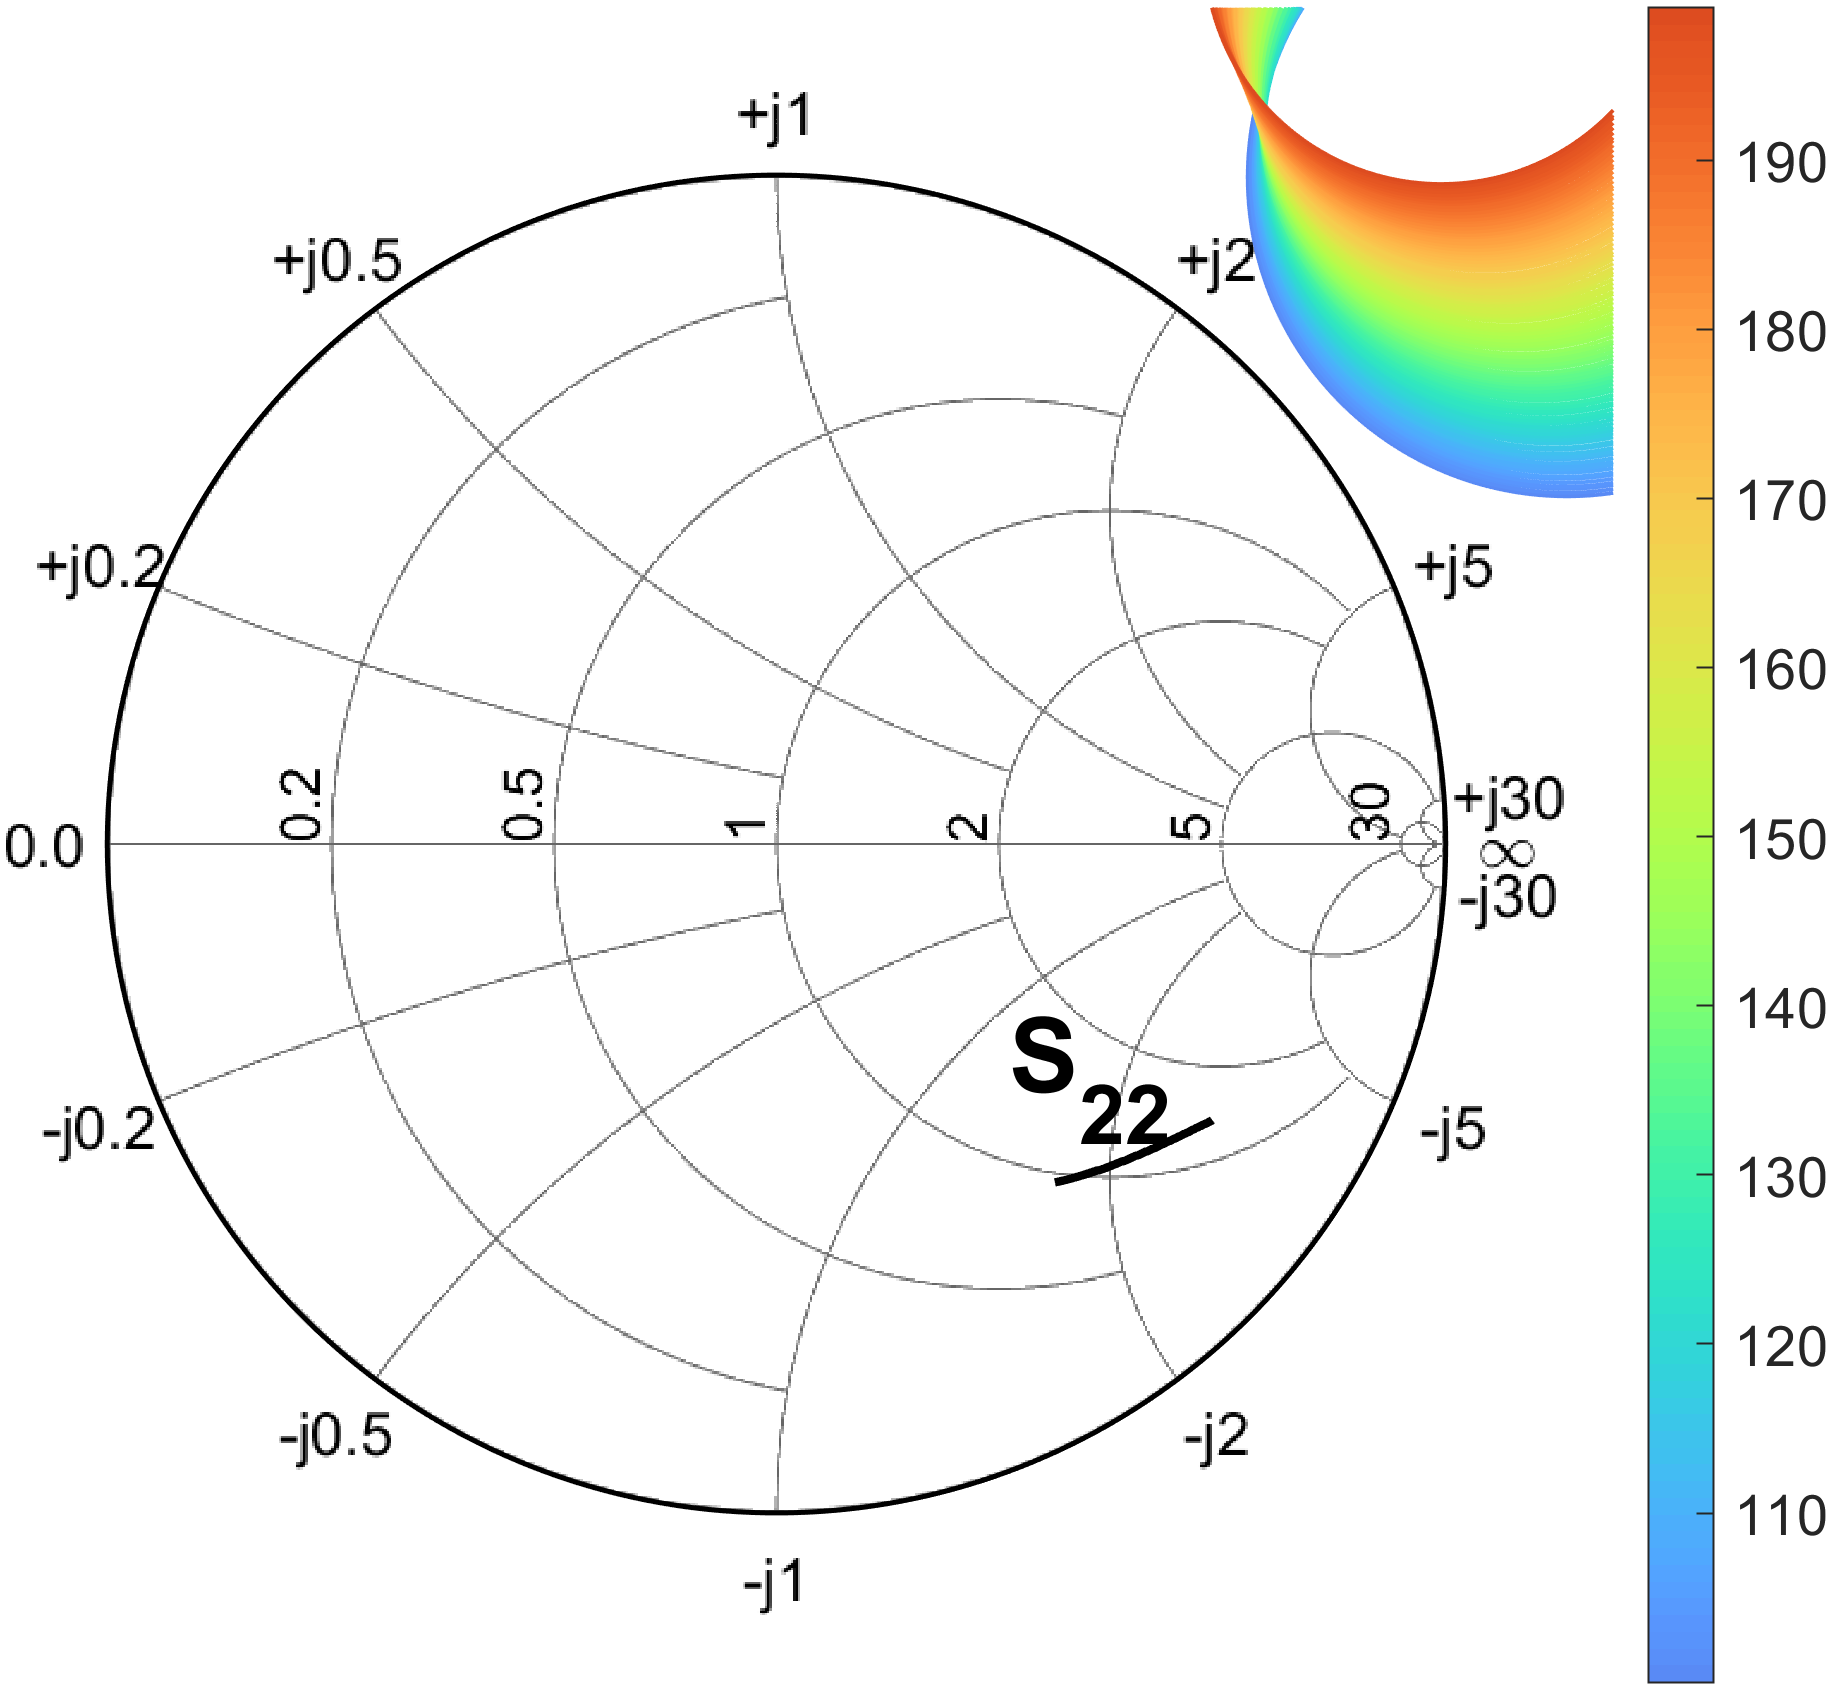
\includegraphics[width=0.95\linewidth]{Design_figures/Measurements/SecondStage/EM_DiffAmplifier1_ExtractPar_LongInputTM2_S_MaxGain_S21_LoadStability.png}
        \caption{}
        \label{fig:EM_DiffAmplifier1_ExtractPar_LongInputTM2_S_MaxGain_LoadStability}
    \end{subfigure}
    \caption{Simulated results of the (a) source and (b) load stability circles for the layout of the double-input balanced-output differential amplifier.}
\end{figure}
%
%The stability simulations does not change with the addition of \SI{10}{\ohm} resistor represented as losses at the output. these results are presented in Appendix.\ref{sec:Appendix}

\begin{comment}
\paragraph{given the results of Second stage...approx circuit of first stage (mettere dopo)}
The imbalance of the first stage can be associated to intrinsic imbalances of the topology as the single input At $Q_1$ and the shunt capacitor at Q2.
\textcolor{red}{ da riesaminare con simulazioni. la soluzione stà nell'aggiunta della linea di trasmissione e da C2, le perdite all'emettitore introducono L e diminuiscono gain}
To understand how this is possible, a qualitative approximation of the lines surrounding the core, the transmission line between the emitters and the one going outside the collector are done.
in the figure XX its possible to observe the schematic results of the model with lumped elements.
The difference is mostly done by the parasitic capacitance at the emitter, meanshilw the inductances 

\begin{figure}[!hbt]
    \centering
    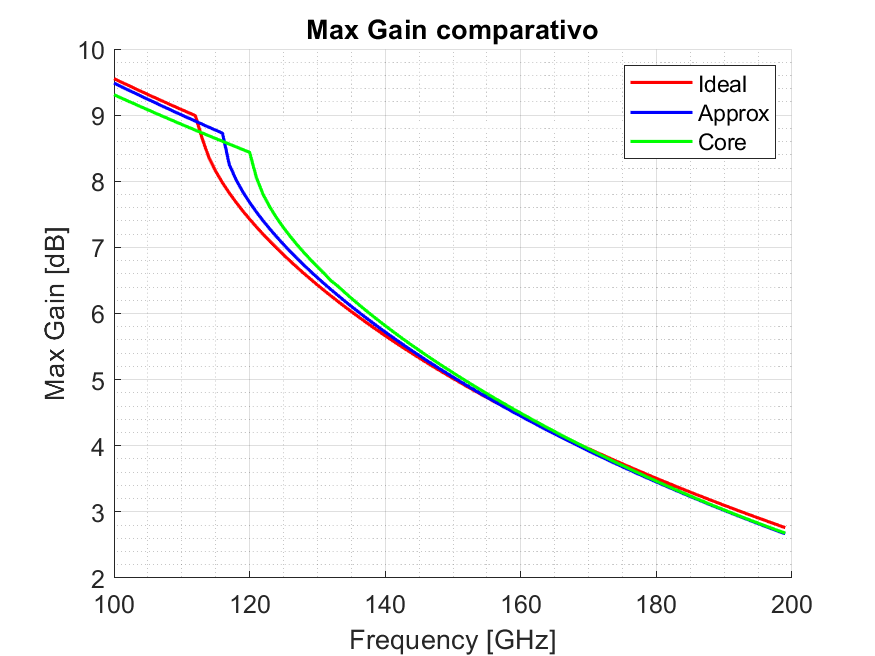
\includegraphics[width=0.5\linewidth]{Design_figures/Measurements/FirstStage/FirstStage_Ideal_VS_EM_MaxGain_Comparativo.png}
    \caption{Caption}
    \label{fig:placeholder}
\end{figure}
\\
\begin{figure}[!hbt]
    \centering
    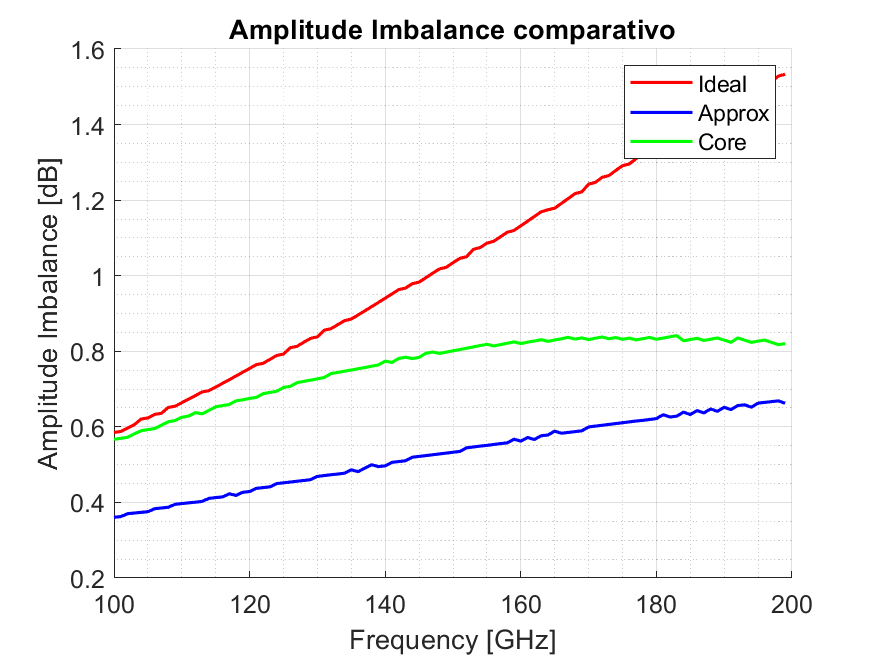
\includegraphics[width=0.5\linewidth]{Design_figures/Measurements/FirstStage/FirstStage_Ideal_VS_EM_AmplitudeImbalance_Comparativo.png}
    \caption{Caption}
    \label{fig:placeholder}
\end{figure}
\\
\begin{figure}[!hbt]
    \centering
    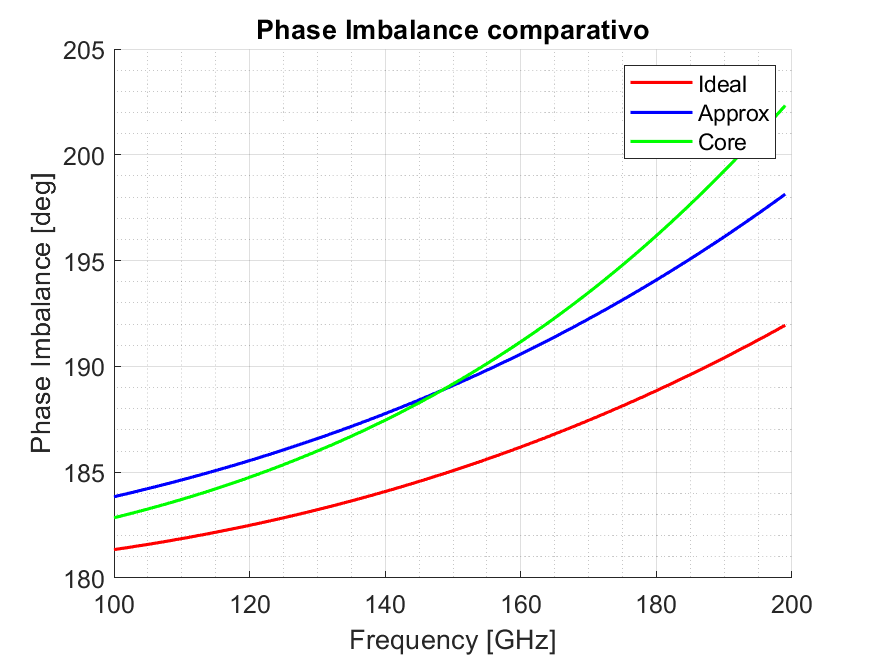
\includegraphics[width=0.5\linewidth]{Design_figures/Measurements/FirstStage/FirstStage_Ideal_VS_EM_PhaseImbalance_Comparativo.png}
    \caption{Caption}
    \label{fig:placeholder}
\end{figure}
\end{comment}
%%%%
\cleardoublepage
\subsubsection{Layout of the third stage}
\label{subsubsec:Layout of the third stage}
%%%%%%%%%%%%%%%%%%%%%%%%%%%%%%%%%%%%%%%%%%%%
\label{Layout_level_of_the_third_stage}
Figure \ref{fig:LayoutThirdAmplifier} illustrates two layouts made in different periods.
The layout structure is identical in both figures except for the middle component which connects the transistor's bases to each other and to the biasing network. 
\begin{figure}[htbp!]
    \centering
    \begin{minipage}[c]{0.49\linewidth}
        \centering
        \begin{overpic}[width=0.8\linewidth]{Design_figures/Layout/LayoutThirdStage/LayoutThirdStageOLD.png}
\put(20,65){\makebox(0,0){(\textcolor{white}{L1})}}
\put(20,35){\makebox(0,0){(\textcolor{white}{L2})}}
\put(21.25,60.5){\makebox(0,0){(\textcolor{white}{Q9})}}
\put(21.25,46){\makebox(0,0){(\textcolor{white}{Q10})}}
\put(15,47.5){\makebox(0,0){(\textcolor{white}{R10})}}
\put(15,54.5){\makebox(0,0){(\textcolor{white}{R9})}}
\put(18,50){\makebox(0,0){(\textcolor{white}{C})}}
            
        \end{overpic}
        \caption*{(a)}
    \end{minipage}
    \hfill
    \begin{minipage}[c]{0.39\linewidth}
        \centering
        \begin{overpic}[width=0.8\linewidth]{Design_figures/Layout/LayoutThirdStage/ZoomCoreThirdStage.png}
%            \put(13,30){\makebox(0,0){(\textcolor{white}{X})}}
%            \put(13,76.5){\makebox(0,0){(\textcolor{white}{X})}}
%            \put(51,30){\makebox(0,0){(\textcolor{white}{X})}}
%            \put(51,76.5){\makebox(0,0){(\textcolor{white}{X})}}
            \put(36.5,94){\makebox(0,0){(\textcolor{white}{L1})}}
            \put(36.5,7){\makebox(0,0){(\textcolor{white}{L2})}}
            \put(39,84){\makebox(0,0){(\textcolor{white}{Q9})}}
            \put(39,37){\makebox(0,0){(\textcolor{white}{Q10})}}
            \put(26.5,42.5){\makebox(0,0){(\textcolor{white}{R10})}}
            \put(26.5,58.5){\makebox(0,0){(\textcolor{white}{R9})}}
            
        \end{overpic}
        \caption*{(b)}
    \end{minipage}

    \caption{Illustration of the CB amplifier layout in a symmetric configuration: (a) the previous implementation with a shunt capacitor; (b) the realized version with a metal transmission line.}
    \label{fig:LayoutThirdAmplifier}
\end{figure}
\\
The layout is designed as it follows: 
the collector of each transistor is routed to their respective ports in the right side by a path consisting of Metal1, via Metal1-to-TopMetal2 and TopMetal2.
The input ports on the left side are routed to the emitters by a path consisting of TopMetal2, via TopMetal2-to-Metal2 and Metal2. Furthermore, the emitter of each transistor is connected to an Inductor-like transmission line through the via between Metal2 and TopMetal2. These $L1$ and $L2$ inductors are realized in the TopMetal2 layer and are terminated to the RF ground by vias. The inductors are designed in a spiral way so as to achieve higher inductance through coupling effect and to make it compact.\\
In Appendix \ref{sec:Appendix}, Figure \ref{fig:LayoutSpiral_vs_Line_indcutorComponent}, \ref{fig:LayoutSpiral_vs_Line_indcutorComponent_measureL&R} and  \ref{fig:LayoutSpiral_vs_Line_indcutorComponent_measureQ}, 
it's possible to check the layout and results of the spiral inductor in comparison to a straight transmission line, from which it is possible to see how this latter solution permits a contained value around $\SI{80}{\pH}$ with lower losses indicated by the high quality factor Q. The latter configuration was ultimately not chosen because achieving a higher inductance was more important. 
\\
\textcolor{white}{newline newline}
\\
During the layout design, it was noted that the third stage output impedances were very small, with the real part being around \SI{10}{\ohm}. This result complicated the creation of simple matching networks, leading to the idea of changing the shunt capacitor value.
\begin{figure}[hbt!]
    \centering
    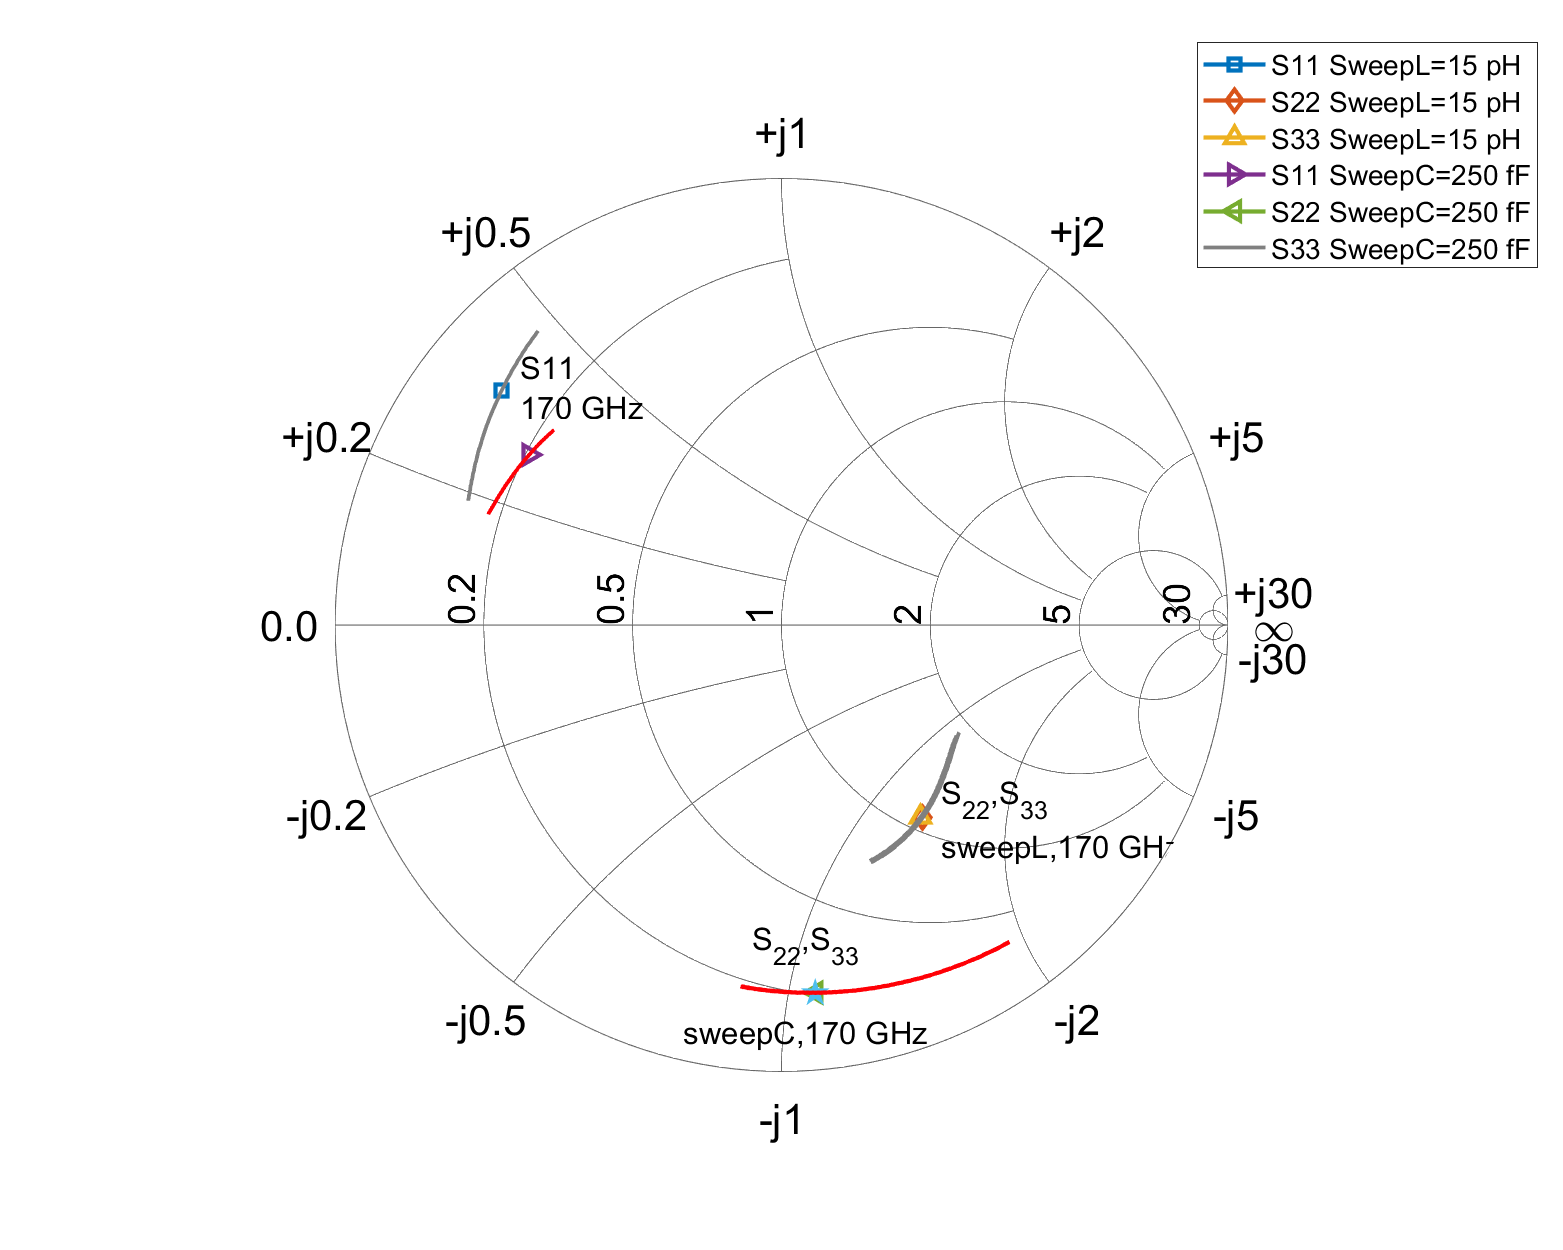
\includegraphics[width=0.75\linewidth]{Design_figures/Measurements/ThirdStage/SmithPlot_AllSweeps_Comparison.png}
    \caption{Smith chart of the deviation in the input and output impedances with an ideal \SI{250}{\femto\farad} shunt capacitor versus an ideal \SI{15}{\pico\henry} inductor.}
    \label{fig:SmithPlot_AllSweeps_ComparisonText}
\end{figure}
\\
A temporary layout, illustrated in Appendix \ref{sec:Appendix} Figure \ref{fig:cb_amplifier_sweeps}.a, was implemented without any component at the middle but with external ports to examine the circuit's behaviour with an ideal shunt capacitor.\\
By sweeping this ideal $C$ from \SI{250}{\pF} down to \SI{25}{pF}, the overall MaxGain did not get affected due to a supposed virtual ground between the transistors bases. Given this result, the remotion of this component in favor of a path constituted by a small Metal1 transmission line was taken into account.
Furthermore, a test with an ideal inductor, in Appendix \ref{sec:Appendix} Figure \ref{fig:cb_amplifier_sweeps}.b, was made to check if the design would be affected by the line. The results are shown in Figure \ref{fig:Comparison_ThirdStage_MaxGain_MultiSweepL_C}. 
\begin{figure}[hbt!]
    \centering
    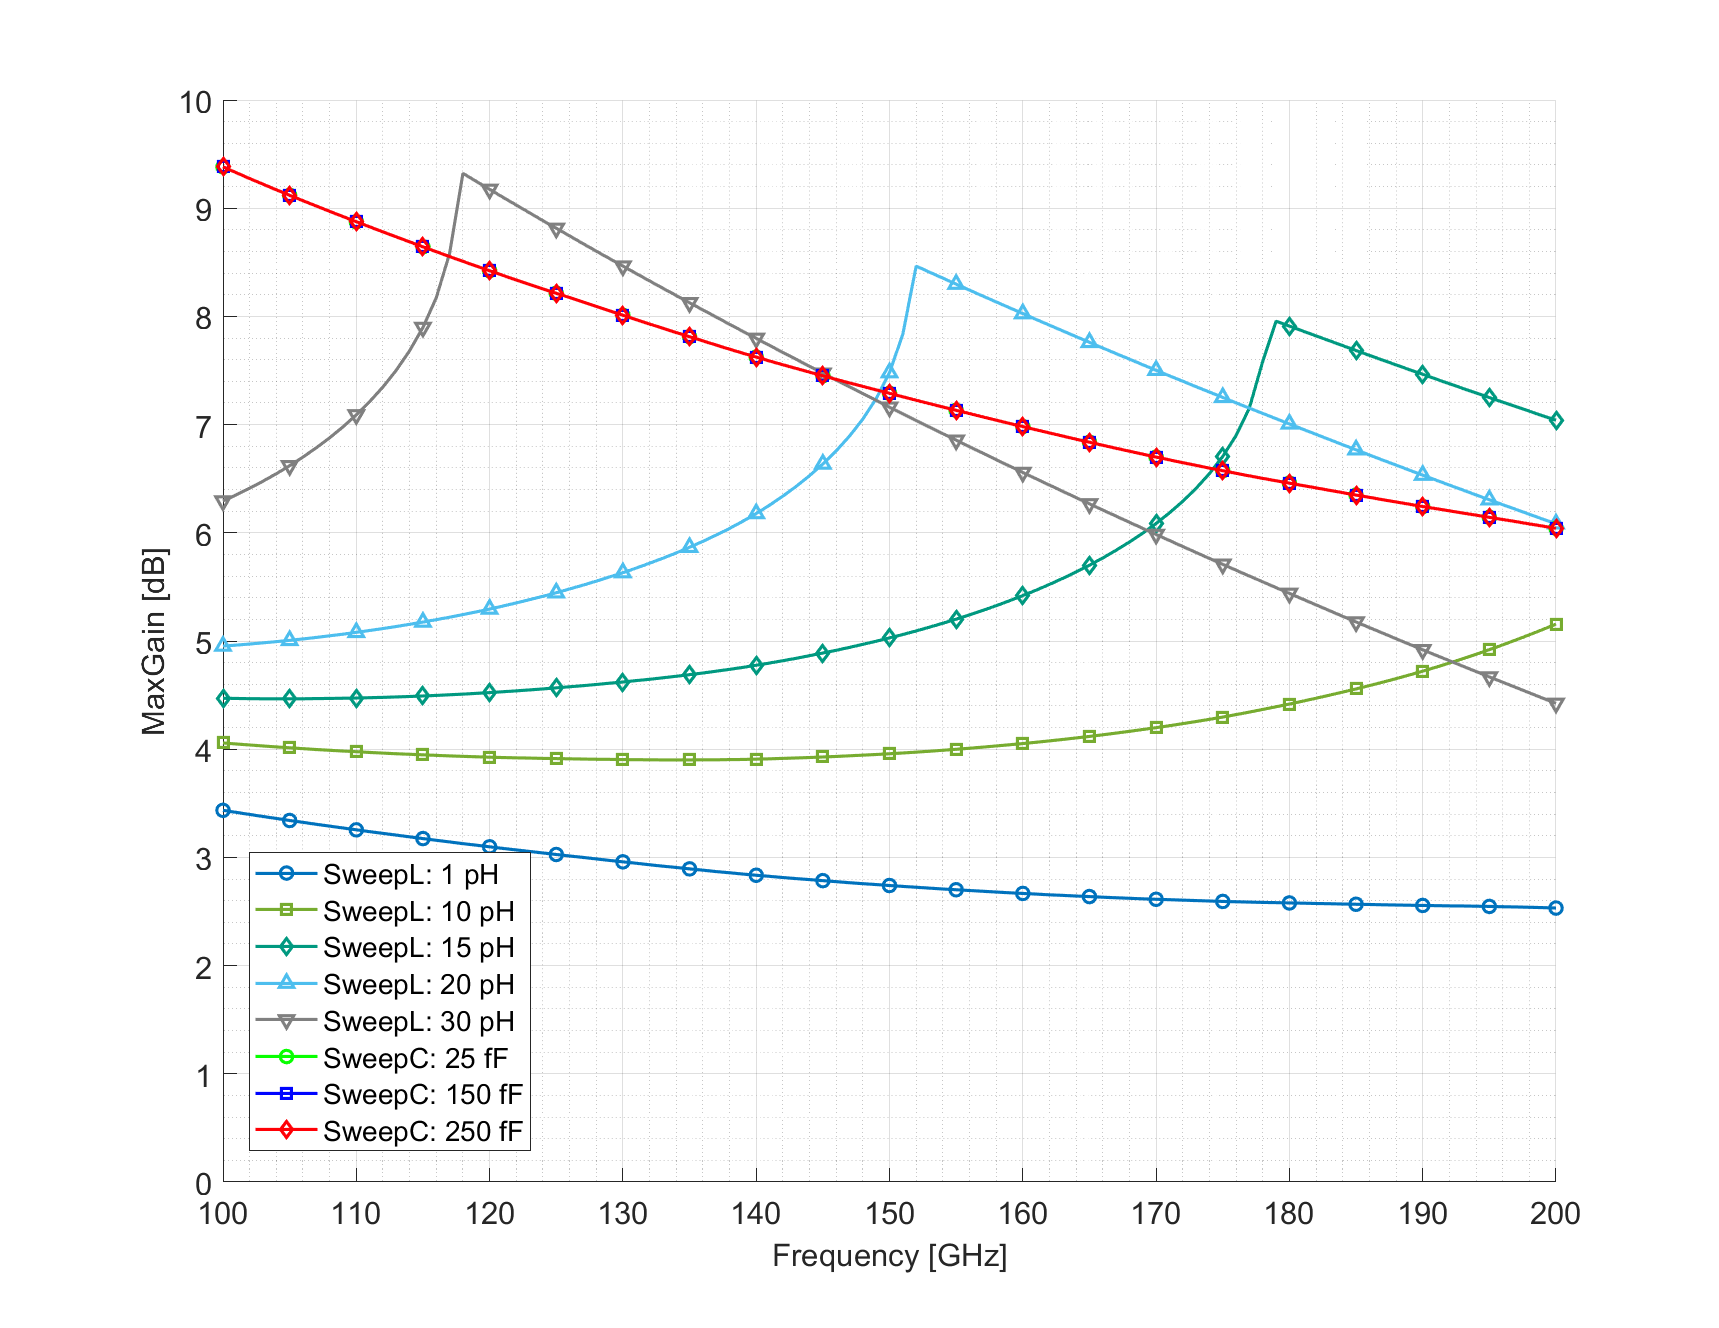
\includegraphics[width=0.7\linewidth]{Design_figures/Measurements/ThirdStage/Comparison_ThirdStage_MaxGain_MultiSweepL_C.png}
    \caption{Comparison of the MaxGain behaviour for different values of the ideal shunt capacitor and ideal series-line inductor.}
    \label{fig:Comparison_ThirdStage_MaxGain_MultiSweepL_C}
\end{figure}
\\
As shown in Figure \ref{fig:SmithPlot_AllSweeps_ComparisonText}, the implementation of the ideal inductor line significantly increases the output impedance, simplifying the design of future matching networks.\\
\begin{comment}
During the design process, this step was not considered carefully enough because the focus was mainly on the overall design imbalance and on the output impedance. As a result, the change in the MaxGain of the single stage was overlooked. Nevertheless, in retrospect, it is likely that the same configuration would have been selected between the two alternatives.\\
\end{comment}
By comparing the MaxGain trends obtained with ideal components, shown in Figure~\ref{fig:Comparison_ThirdStage_MaxGain_MultiSweepL_C}, with the MaxGains extracted from the layouts in Figure~\ref{fig:LayoutThirdAmplifier} and shown in Figure~\ref{fig:processEM_ThirdStage_CompareMidCap_VS_inductorLineComputed_MAG_MSG_Comparison.png}, it is possible to conclude that the effect on MaxGain is caused by the stability behaviour of the stage. The implementation of the line results in the increase of stability factor, leading to an unconditionally stable network and bringing MaxGain to become the MAG in equation (\ref{eq:MAG}).
The network of the layout with the EM capacitor, on the other hand, was in a conditional stable situation as its MaxGain matches with the MSG.
\begin{figure}[hbt!]
    \centering
    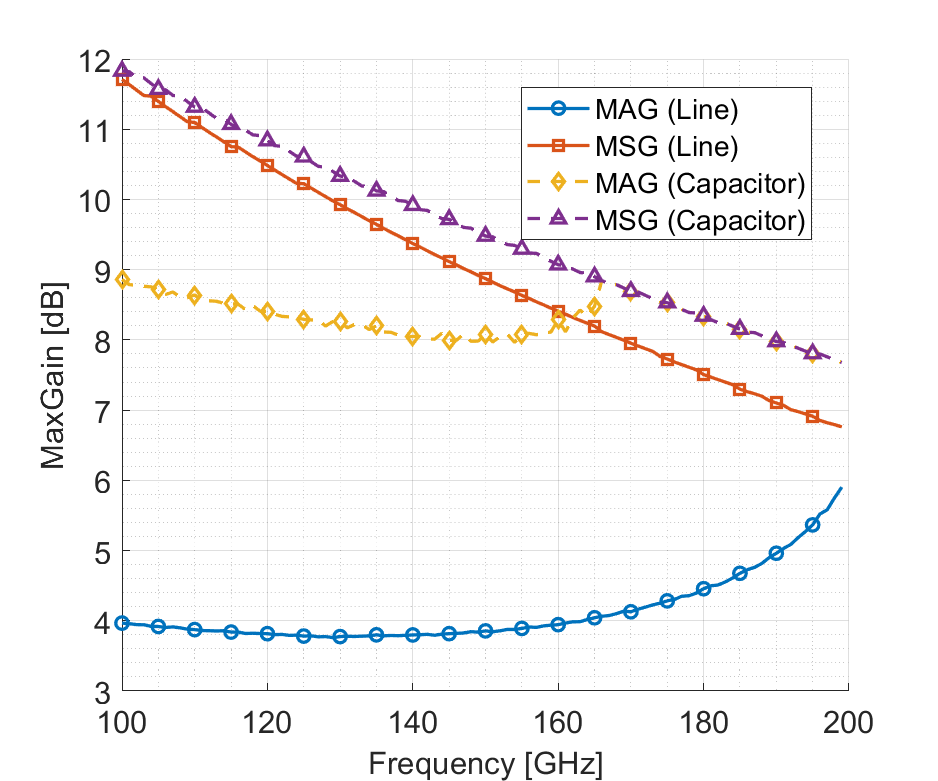
\includegraphics[width=0.65\linewidth]{Design_figures/Measurements/ThirdStage/processEM_ThirdStage_CompareMidCap_VS_inductorLineComputed_MAG_MSG_Comparison.png}
    \caption{MAG and MSG simulations of the third stage layout with an EM capacitor versus an EM line.}
    \label{fig:processEM_ThirdStage_CompareMidCap_VS_inductorLineComputed_MAG_MSG_Comparison.png}
\end{figure}

Per definition of (\ref{eq:MSG}), the MSG is calculated with K=1. This explains why the MSG of the capacitor and that of the line are relatively similar in the lower half of the frequency range, whereas at higher frequencies the line exhibits losses of nearly $1_{dB}$, supposedly because the line starts to significantly degrade $|S_{12}|$.
The MAG trends, on the contrary, are very different. The capacitor shows a much higher MAG, relatively close to the MSG, suggesting that the EM capacitor leads to a lower stability factor in the circuit compared with the transmission line.\\
To support this observation, stability factor simulations were carried out and are presented in Figure \ref{fig:EMCBamplifier_ExtractPar_Symmetric_Finger6_StabilityS21_K_Mu_Stability}.

\begin{figure}[hbt!]
    \centering
        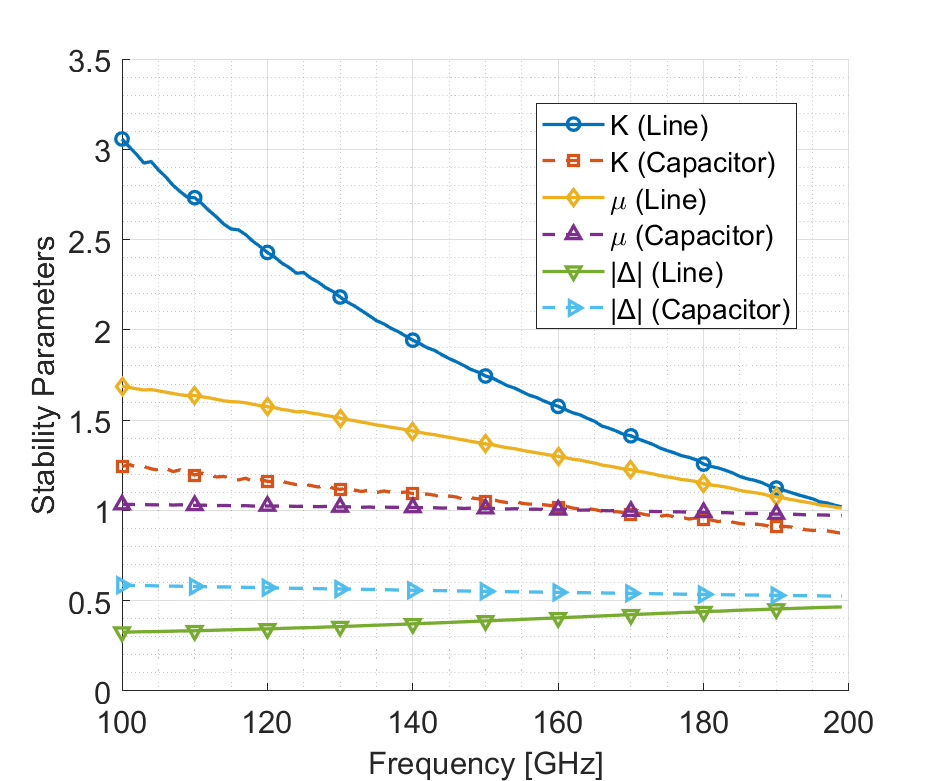
\includegraphics[width=0.65\linewidth]{Design_figures/Measurements/ThirdStage/processEM_ThirdStage_CompareMidCap_VS_inductorLineStability_Metrics_Comparison.png}
        \caption{Stability parameters of the third stage layout with an EM capacitor versus an EM line.}
        \label{fig:EMCBamplifier_ExtractPar_Symmetric_Finger6_StabilityS21_K_Mu_Stability}
\end{figure}

More informations regarding K, $\mu$,$\mu'$, MAG and MSG for the Etwo different EM cases are shown in Appendix \ref{sec:Appendix}, Figure \ref{fig:processEM_ThirdStage_CompareMidCap_VS_inductorLineStability_Metrics_Comparison.png} and 
\ref{fig:processEM_ThirdStage_CompareMidCap_VS_inductorLineStability_and_Gain_Comparison.png}.
\begin{comment}
    \begin{figure}[hbt!]
    \centering
    \begin{subfigure}{0.49\textwidth}
        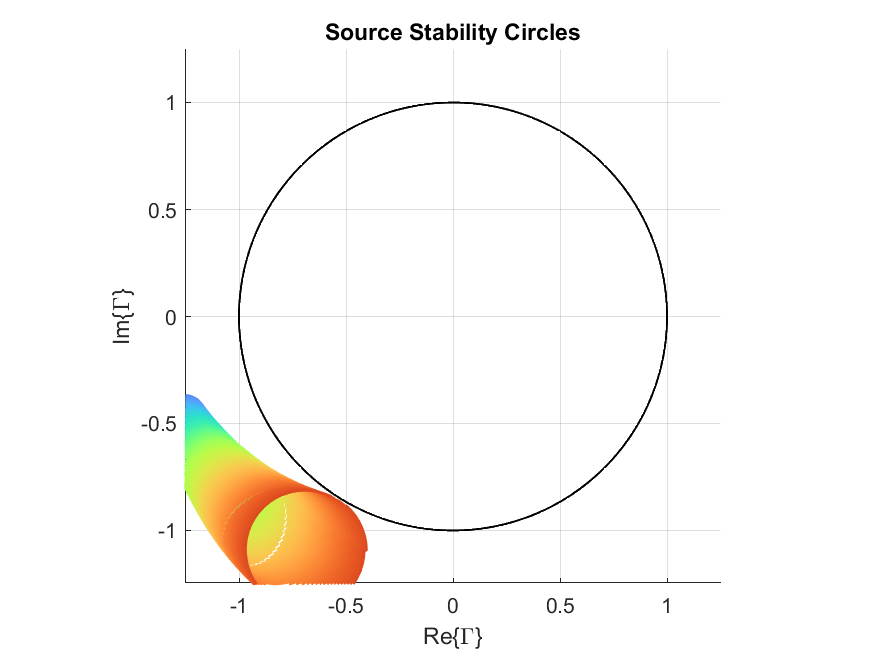
\includegraphics[width=\linewidth]{Design_figures/Measurements/ThirdStage/EMCBamplifier_ExtractPar_Symmetric_Finger6_StabilityS21_Source_Stability_Circles.png}
        \caption{}
        \label{}
    \end{subfigure}
    \hfill
    \begin{subfigure}{0.49\textwidth}
        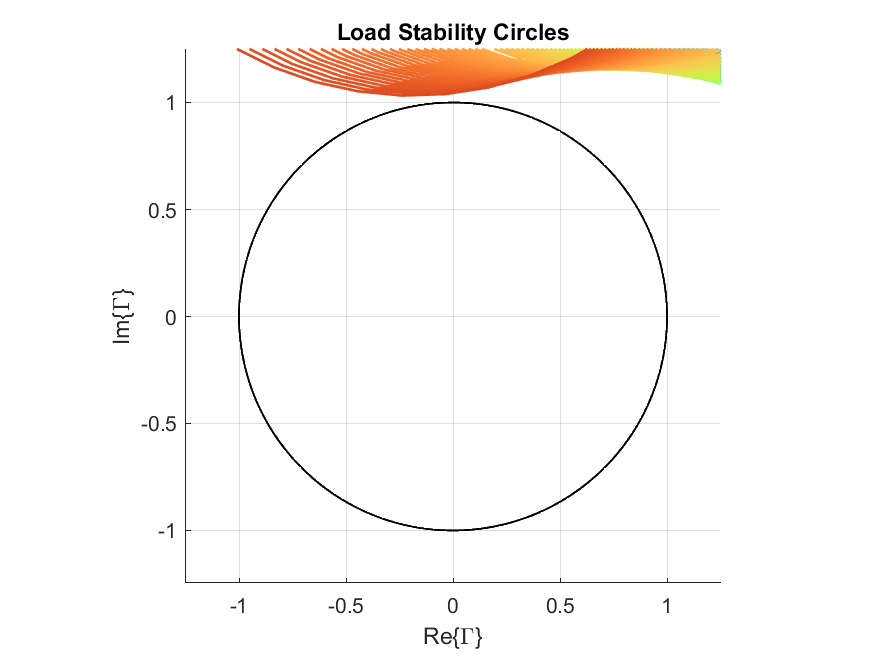
\includegraphics[width=\linewidth]{Design_figures/Measurements/ThirdStage/EMCBamplifier_ExtractPar_Symmetric_Finger6_StabilityS21_Load_Stability_Circles.png}
        \caption{}
        \label{}
    \end{subfigure}
    \caption{Caption}
    \label{fig:placeholder}
\end{figure}
\end{comment}


\cleardoublepage
\subsection{Combined analysis of merged stages}
\label{sec:Combined_Analysis_of_merged_stages Analysis_combined_core}
%
%%%%%%%%%%%%%%%%%%%%%%%%%%%%%%%%%%%%%%%%%%%%%%%%%%%%%%%%%%%%%%%%%%%
Once the independent stages are analyzed, a check of their combination is fundamental to verify whether the overall parameters improves accordingly to the theoretical design, and how much they differentiate. 
For a complete analysis, there are also going to be comparisons without the third stage, in which the outputs of the second differential are connected to the load terminations.
It's expected an improvement of the balance after the second stage, and only an improvement of gain after the third stage.\\
The schematic level design is shown in Figure \ref{fig:SchematicFullDesign} while its counterpart with EM cores is shown in Figure \ref{fig:LayoutSchematic_level_of_Complete_Circuit_Project}. This last schematic has some differences from the ideal one: they both are simulated without matching networks but in Figure \ref{fig:LayoutSchematic_level_of_Complete_Circuit_Project}, \SI{10}{\ohm} resistors are placed at every feed line in the prevision of losses that would have been caused by the layout matching networks and by the layout block capacitors; furthermore the ideal circuit in Figure \ref{fig:SchematicFullDesign} implements a shunt capacitor at the third stage meanwhile, as described in the paragraph \ref{Layout_level_of_the_third_stage}, the effective third stage core used in the tapeout is implemented with only a Metal1 transmission line, Figure \ref{fig:LayoutSchematic_level_of_Complete_Circuit_Project}.

\begin{figure}[hbt!]
\centering
\begin{adjustbox}{max width=\textwidth}
  \begin{circuitikz}[transform shape]
    \draw (0,0) node[npn, xscale=1, anchor=B] (Q1)
    {\shortstack{$Q1$ \\ 2}};
    %metto metà sinistra dell'emettitore
    \draw (Q1.E)--++(0,-0.35)--++(1.1,0) coordinate(e);
    %metto metà destra dell'emettitore e Q2
    \draw(e)--++(1.1,0) --++(0,+0.35) node[npn, xscale=-1, anchor=E] (Q2){\ctikzflipx{\shortstack{$Q2$ \\ 2}}};
    %disegno current mirror
    \draw (e) to [short,*-]++(0,-0.25) node[npn, xscale=1, anchor=C] (Q3)
    {\shortstack{$Q3$ \\ 2}};
    \draw (Q3.E) --++(0,-0.5) node[npn, xscale=1, anchor=C] (Q4){\shortstack{$Q4$ \\ 2}} ;
    \draw (Q4.E) --++(0,-0.15) node[tlground]{};

    %inserisco le resistenze bias AC block
    %biasin a Q1
    \draw (Q1.B)--++(-0.85,0) coordinate (in1)
    to [R,l=$\mathrm{R}_1$,*-]++(0,1.5)
    to [open]++(-0.35,0) --  node[anchor=south] {$\mathrm{V}_{\mathrm{CC}}$} ++(0.7,0);
    %biasing a Q2
    \draw (Q2.B)--++(0.85,0) coordinate (in2)
    to [R,l=$\mathrm{R}_2$]++(0,1.5) to [open]++(-0.35,0) --  node[anchor=south] {$\mathrm{V}_{\mathrm{CC}}$} ++(0.7,0);
    %biasing current mirror Q3
    \draw (Q3.B) to [short]++(-0.15,0) coordinate (in3);
    \draw (in3)--++(-0.25,0) to [R,l_=$\mathrm{R}_3$]++(-2,0) to [short,-o]++(-0.25,0) node[left]{$\mathrm{V}_{\mathrm{B2}}$};
    \draw (in3) to [C,l_=$C_{1}$,*-]++(0,-1.25)node[tlground]{};
    %biasing current mirror Q4
    \draw (Q4.B) to [R,l_=$\mathrm{R}_4$]++(-1.25,0) to [short,-o]++(-0.25,0) node[left]{$\mathrm{V}_{\mathrm{B1}}$};
    %inserisco input a base Q1
    \draw (in1) to [C,*-o] ++(-2,0) coordinate(dc1)node[left]{$v_{se}$};
    
    \draw (dc1) to [open]++(0.475,-0.375) rectangle++(1.05,0.75);
    %inserisco capacità a base Q2
    \draw (in2)++(-0.5,0) to [C,l=$C_{2}$,*-]++(0,-1.25)node[ground]{};

    %disegno collettore Q1
    \draw (Q1.C) --++ (0,1.75) coordinate(c1) to [L]++(0,2) to [open]++(-0.35,0) --  node[anchor=south] {$\mathrm{V}_{\mathrm{CC}}$} ++(0.7,0);
    
    
    \draw (Q2.C) --++ (0,1.25) coordinate(c2)--++(0,0.5) to [L]++(0,2) to [open]++(-0.35,0) --  node[anchor=south] {$\mathrm{V}_{\mathrm{CC}}$} ++(0.7,0);


%%%%%%%%%%%%% secondo stadio
\draw (8.5,0) node[npn, xscale=1, anchor=B] (Q5)
    {\shortstack{$Q5$ \\ 2}};
    %metto metà sinistra dell'emettitore
    \draw (Q5.E)--++(0,-0.35)--++(1.1,0) coordinate(e2);
    %metto metà destra dell'emettitore e Q6
    \draw(e2)--++(1.1,0) --++(0,+0.35) node[npn, xscale=-1, anchor=E] (Q6){\ctikzflipx{\shortstack{$Q6$ \\ 2}}};
    %disegno current mirror
    \draw (e2) to [short,*-]++(0,-0.25) node[npn, xscale=1, anchor=C] (Q7)
    {\shortstack{$Q7$ \\ 2}};
    \draw (Q7.E) --++(0,-0.5) node[npn, xscale=1, anchor=C] (Q8){\shortstack{$Q8$ \\ 2}} ;
    \draw (Q8.E) --++(0,-0.15) node[tlground]{};

    %inserisco le resistenze bias AC block
    %biasin a Q5
    \draw (Q5.B)--++(-0.85,0) coordinate (2in1)
    to [R,l=$\mathrm{R}_5$,*-]++(0,1.5)
    to [open]++(-0.35,0) --  node[anchor=south] {$\mathrm{V}_{\mathrm{CC}}$} ++(0.7,0);
    %biasing a Q6
    \draw (Q6.B)--++(0.85,0) coordinate (2in2)
    to [R,l=$\mathrm{R}_6$]++(0,1.5) to [open]++(-0.35,0) --  node[anchor=south] {$\mathrm{V}_{\mathrm{CC}}$} ++(0.7,0);
    %biasing current mirror Q7
    \draw (Q7.B) to [short]++(-0.15,0) coordinate (2in3);
    \draw (2in3)--++(-0.25,0) to [R,l_=$\mathrm{R}_7$]++(-2,0) to [short,-o]++(-0.25,0) node[left]{$\mathrm{V}_{\mathrm{B2}}$};
    \draw (2in3) to [C,l_=$C_{1}$,*-]++(0,-1.25)node[tlground]{};
    %biasing current mirror Q8
    \draw (Q8.B) to [R,l_=$\mathrm{R}_8$]++(-1.25,0) to [short,-o]++(-0.25,0) node[left]{$\mathrm{V}_{\mathrm{B1}}$};
    %inserisco input a base Q5
    \draw (2in1) to [C] ++(-1.6,0) coordinate(2vin1);
    \draw (2vin1) to [open]++(0.275,-0.375) rectangle++(1.05,0.75);
    %creo nodo base Q6
    \draw (2in2) to [open,-*]++(-0.5,0) coordinate(2vin2);
    
    %disegno collettore Q1
    \draw (Q5.C) --++ (0,1.75) coordinate(2c1) to [L]++(0,2) to [open]++(-0.35,0) --  node[anchor=south] {$\mathrm{V}_{\mathrm{CC}}$} ++(0.7,0);
   
    \draw (Q6.C) --++ (0,1.25) coordinate(2c2)--++(0,0.5) to [L]++(0,2) to [open]++(-0.35,0) --  node[anchor=south] {$\mathrm{V}_{\mathrm{CC}}$} ++(0.7,0);
    
%% collego i due stadi
\draw (c1) to [short,*-]++(5,0)--++(0,-2.52) -|(2vin1);

\draw (c2) to [short,*-]++(2.5,0)--++(0,-3.4)--++(0.5,0)coordinate (dc2)to [C] ++(1.6,0) --++(5,0)-|(2vin2);
    
    
    \draw (dc2) to [open]++(0.275,-0.375) rectangle++(1.05,0.75);

    %riquadri
    \draw (0.425,2.9)rectangle++(0.75,1.25);
    \draw (0.425+2.2,2.9)rectangle++(0.75,1.25);
    
    \draw (0.425+8.5,2.9)rectangle++(0.75,1.25);
    \draw (0.425+8.5+2.2,2.9)rectangle++(0.75,1.25);

%%%%%%%%% TERZO STADIO

   \draw (0+17.25,1) node[npn, yscale=-1, anchor=B] (Q9)
  {\reflectbox{\rotatebox{180}{\shortstack{Q9 \\ 6}}}};
    %inserisco ramo base di Q9
    \draw (Q9.B) to [short]++(-0.35,0) coordinate (vb9);
\draw (vb9) to [R,l_=$\mathrm{R}_9$,*-o]++(-2.2,0) node[left]{$\mathrm{V}_{\mathrm{B}}$};
    
     %inserisco shunt C a comune
    \draw (vb9) --++(0,-1.5) coordinate (x);
    \draw (x) to [C,l_=$C_3$,*-]++(-2,0)node[rotate=-90, tlground]{};
    
    %inserisco ramo collettore Q9
    \draw (Q9.C) --++ (0,-0.25) to [short]++(1.5,0)coordinate(9c1) 
    to [L,*-,mirror]++(0,2) to [open]++(-0.35,0) --  node[anchor=south] {$\mathrm{V}_{\mathrm{CC}}$} ++(0.7,0);
    \draw (9c1) --++(0.05,0) to [C,-o]++(2,0) node[right]{$v_\mathrm{out+}$};
    
    %inserisco ramo emettitore di Q1
    \draw (Q9.E) --++(0,0) coordinate (9in1);
    \draw (9in1) --++ (0,0.75) coordinate(9e1) to [L,mirror]++(0,2.3) node[yscale=-1, tlground]{};
    \draw (9e1) to [C,*-]++(-2,0) node[left]{}coordinate (9Vin);

%ricreo il circuito mirrored
\begin{scope}[shift={(0,-3)}, yscale=-1, transform shape]
\draw (0+17.25,-1) node[npn, yscale=-1, anchor=B] (Q10)
    {\shortstack{$Q10$ \\ 6}};
    %inserisco ramo base di Q1
    \draw (Q10.B) to [short]++(-0.35,0) coordinate (10vb1);
    \draw (10vb1)to [R, l=\reflectbox{\rotatebox{180}{$\mathrm{R}_{10}$}},*-o ,label distance=-6.5mm]++(-2.2,0) node[left]{\reflectbox{\rotatebox{180}{$\mathrm{V}_{\mathrm{B}}$}}};
    \draw (10vb1) --++(0,-1.5);
    
    %inserisco ramo collettore Q10
    \draw (Q10.C) --++ (0,-0.25) to [short]++(1.5,0) coordinate(10c2) to [L,*-,mirror]++(0,2) to [open]++(-0.35,0) --  node[anchor=south] {\reflectbox{\rotatebox{180}{$\mathrm{V}_{\mathrm{CC}}$}}} ++(0.7,0);
    \draw (10c2) --++(0.05,0)to [C,-o]++(2,0) node[right]{\reflectbox{\rotatebox{180}{$v_\mathrm{out-}$}}};
    
    %inserisco ramo emettitore di Q1
    \draw (Q10.E) --++(0,0) coordinate (10in1);
    \draw (10in1) --++ (0,0.75) coordinate(10e2) to [L,mirror]++(0,2.3) node[yscale=-1, tlground]{};
    \draw (10e2) to [C,*-]++(-2,0) node[left]{} coordinate (10Vin);
\end{scope}


    %collego secondo stadio a terzo stadio
     \draw (2c1) to [short,*-]++(6,0)-|(9Vin);
     \draw (2c2) to [short,*-]++(2.25,0)--++(0,-5.54)-|(10Vin);
     
   %label L1 e L2
    \draw (9e1)to [open]++(0.75,1.15) node[]{$L1$};
    \draw (10e2)to [open]++(0.75,-1.15) node[]{$L2$};
    
    %riquadri
    \draw (9c1) to [open]++(-0.35,0.35)rectangle++(0.75,1.25);
    \draw (10c2) to [open]++(-0.35,-0.35)rectangle++(0.75,-1.25);

    \draw (9c1) --++(0.05,0) to [open]++(0.5,-0.425) rectangle++(1,0.85);
    \draw (10c2) --++(0.05,0) to [open]++(0.5,-0.425) rectangle++(1,0.85);
    
    \draw (9e1) to [open]++(-0.35,0.5) rectangle ++(0.75,1.25);
    \draw (10e2) to [open]++(-0.35,-0.5) rectangle ++(0.75,-1.25);
    
    \draw (9e1) to [open]++(-0.5,-0.425) rectangle ++(-1,0.85);
    \draw (10e2) to [open]++(-0.5,-0.425) rectangle ++(-1,0.85);

% disegno graph 2 stage 3 stage
 % Aggiungo una graffa orizzontale sotto
  \draw[decorate, decoration={brace, amplitude=10pt, mirror}] 
    (-3,-5.5) --++ (16.5,0) 
    node[midway, yshift=-18pt]{\LARGE{Two-Stage with ideal Cores}};
    \draw[decorate, decoration={brace, amplitude=10pt, mirror}] 
    (-3,-6.5) --++ (24,0) 
    node[midway, yshift=-18pt]{\LARGE{Three-Stage with ideal Cores}};
\end{circuitikz}
\end{adjustbox}
    \caption{Schematic level design of the ideal active balun with shunt capacitor $C_3$ in the third stage}
    \label{fig:SchematicFullDesign}
\end{figure}

\begin{figure}[!hbt]
    \centering
    \begin{tikzpicture}
        % Inserisci l'immagine
        \node (img) at (0,0) {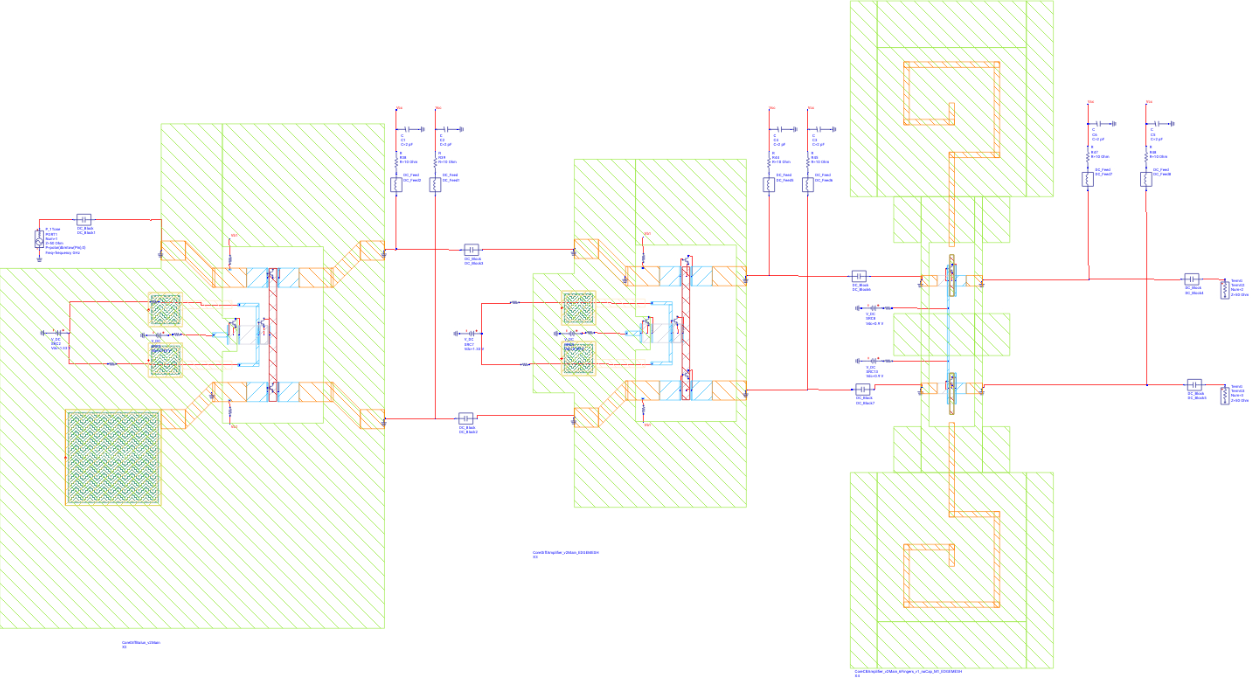
\includegraphics[width=0.95\linewidth]{Design_figures/Layout/Layout3StageMerged_noMN/Layout_3StageMerged_noMN.png}};
        % Seconda graffa sotto un'altra parte (ad esempio secondo stage)
        \draw[decorate, decoration={brace, amplitude=10pt, mirror}] (-7,-3.5) --++ (9,0) node[midway, yshift=-17pt]{Two-Stage with EM Cores}; 
        \draw[decorate, decoration={brace, amplitude=10pt, mirror}] (-7,-4.25) --++ (13,0) node[midway, yshift=-17pt]{Three-Stage with EM Cores};
    \end{tikzpicture}

    \caption{Schematic with EM cores. This schematic does not include the shunt capacitor $C_3$ in the third stage.}
    \label{fig:LayoutSchematic_level_of_Complete_Circuit_Project}
\end{figure}

\begin{figure}[hbt]
    \centering
    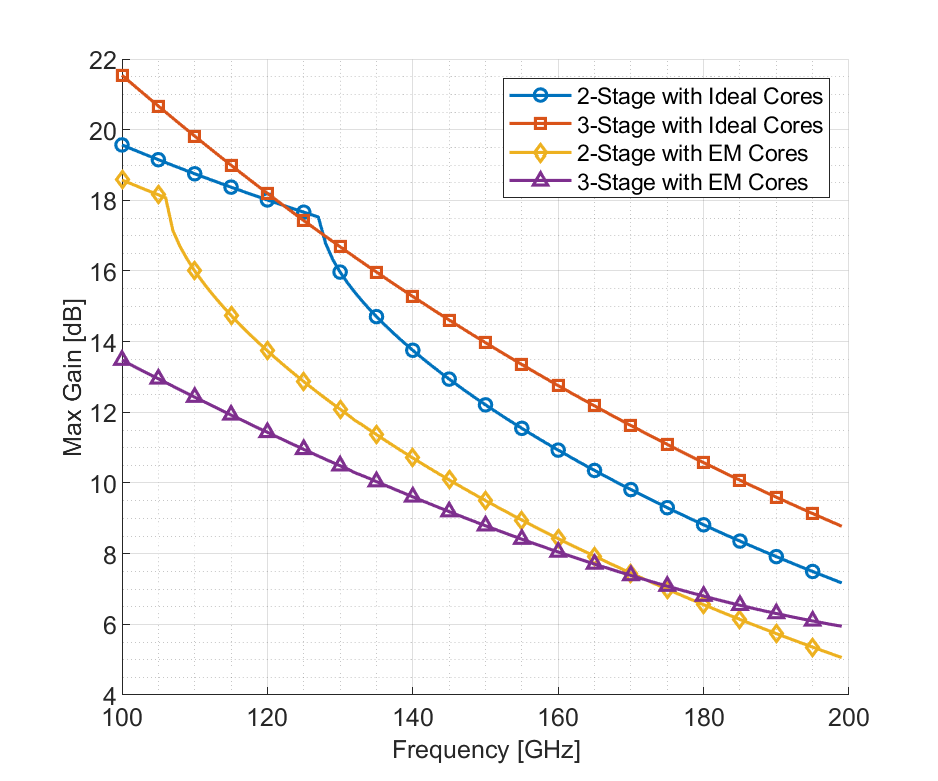
\includegraphics[width=0.5\linewidth]{Design_figures/Layout/ComparisonMeasurements/Comparison_All_MaxGain.png}
    \caption{Deviation of the MaxGain between the ideal and EM-core schematic baluns for the two-stage and three-stage circuit.}
    \label{fig:Schematic_level_of_Complete_Circuit_Project_MeasureComparisons_EM2stage_VS_3stage_MaxGain}
\end{figure}

\paragraph{Main parameters} The results of the Maxgain are shown in Figure \ref{fig:Schematic_level_of_Complete_Circuit_Project_MeasureComparisons_EM2stage_VS_3stage_MaxGain}. The gain discrepancy of the EM two-stage circuit relative to its ideal version is not significant, although a deviation of about 2 dB is observed across the frequency range. 
The gain of the EM three-stage, on the other hand, is significantly affected by the removal of the shunt capacitor and, especially at \SI{100}{\giga\hertz}, a discrepancy of \SI{8}{\decibel} can be noted.\\
It is also necessary to note that the values of this parameter are, by and large, not completely true because, as described in section \ref{sec:Theoretical_Background}, it reflects the maximum value achievable during a lossless conjugate matching at input and output stages, effectively ignoring the possible contribution given by the interstage networks. 
That said, the MaxGain of the 2 Stage balun is ignoring the contribution of the first interstage matching network, and the MaxGain of the 3 stage balun is ignoring the contributions of both the first and second interstage matching networks.

The amplitude imbalances are shown in Figure \ref{fig:Schematic_level_of_Complete_Circuit_Project_MeasureComparisons_EM2stage_VS_3stage_a}.

The improvement in the amplitude imbalance from the ideal first stage stage 1 to the ideal 2-stage network is \SI{1.2}{dB}. The reduction from \SI{1.6}{\decibel} at \SI{200}{\giga\hertz} of the ideal first stage, Figure \ref{fig:FirstStage_Ideal_VS_differentEM_AmplitudeImbalance_Comparativo} to \SI{0.41}{\decibel} at \SI{200}{\giga\hertz} observed by the 2Stage trend in Figure \ref{fig:Schematic_level_of_Complete_Circuit_Project_MeasureComparisons_EM2stage_VS_3stage_a}, is attributed to the enhanced CMRR. The first stage inherently introduces a common-mode component due to the presence of a single input node. This common-mode signal is effectively minimized by the second stage, while the differential component passes through, following the expected theoretical behavior of the circuit.
Furthermore, the general trend of the parameter hasn't changed with the addition of the third stage.

The layout of the first stage presented in Section displayed an amplitude imbalance of \SI{0.5}{\decibel} at \SI{200}{\giga\hertz}. With the addition of the EM simulated second stage, Figure \ref{fig:FirstStage_Ideal_VS_differentEM_AmplitudeImbalance_Comparativo}, the amplitude imbalance goes further down to -0.3dB.
in both the ideal and real cases, the second stage contributed to the reduction of the parameter in equal value, indicating, indicating once again, that EM of the second stage closely matches the ideal behavior, and so it does with the CMRR.

The phase imbalances in Figure \ref{fig:Schematic_level_of_Complete_Circuit_Project_MeasureComparisons_EM2stage_VS_3stage_b} shows the same pattern of the amplitude imbalance, although some investigations revealed that ADS was adding $-360\deg$ to the "2 Stage with ideal core" line, so a mathematical addition of 360 degrees has been applied to the in MATLAB to move it from -180 to 180 deg.

\begin{figure}[hbt]
    \centering
    % Prima immagine
    \begin{subfigure}{0.48\textwidth}
        \centering
        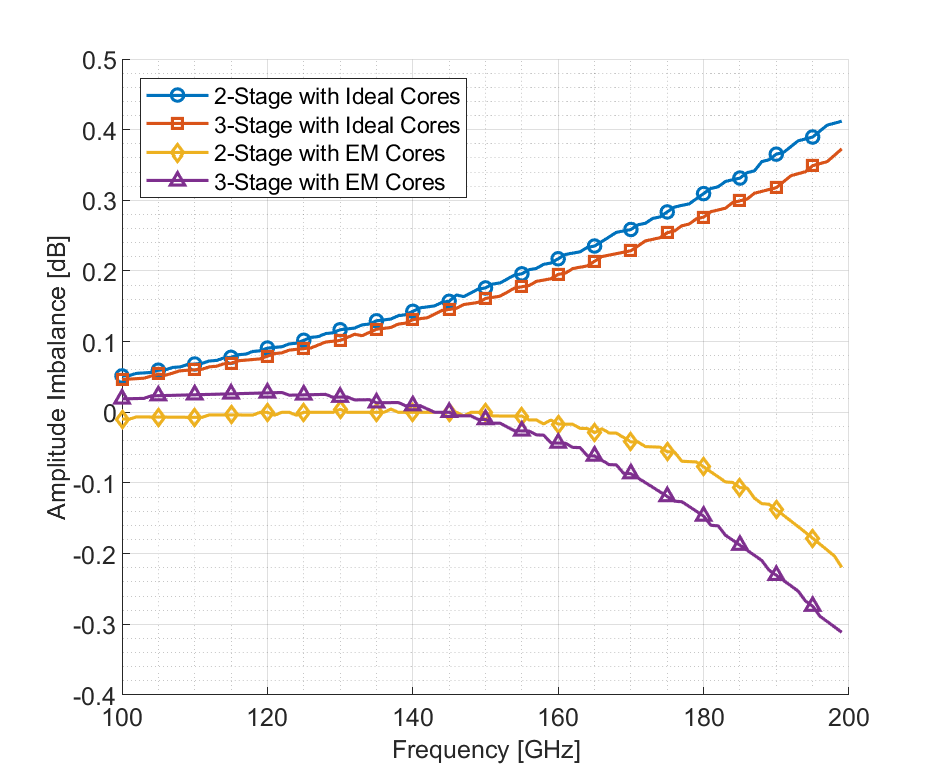
\includegraphics[width=\linewidth]{Design_figures/Layout/ComparisonMeasurements/Comparison_All_AmplitudeImbalance.png}
        \caption{}        \label{fig:Schematic_level_of_Complete_Circuit_Project_MeasureComparisons_EM2stage_VS_3stage_a}
    \end{subfigure}\hfill
    % Seconda immagine
    \begin{subfigure}{0.48\textwidth}
        \centering
        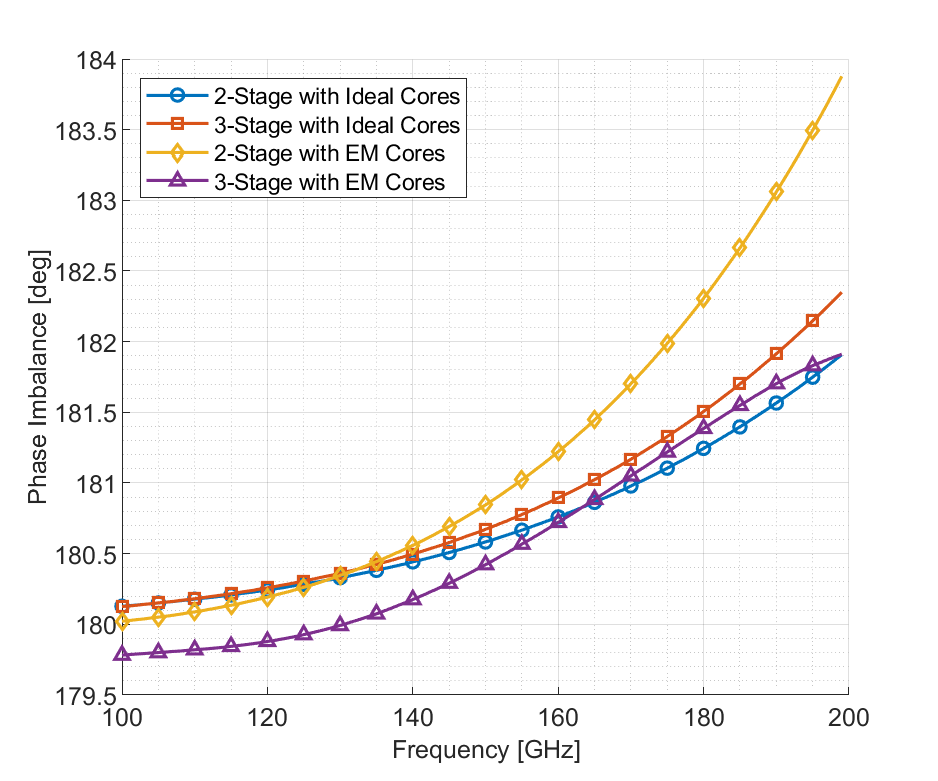
\includegraphics[width=\linewidth]{Design_figures/Layout/ComparisonMeasurements/Comparison_All_PhaseImbalance.png}
        \caption{}        \label{fig:Schematic_level_of_Complete_Circuit_Project_MeasureComparisons_EM2stage_VS_3stage_b}
    \end{subfigure}
    \caption{Ideal and EM core schematic balun parameters for the two-stage and three-stage circuit: (a) amplitude imbalance; (b) phase imbalance.}
\end{figure}
\noindent
%\vspace{0pt}  % forza LaTeX a ripartire da qui
\cleardoublepage
\paragraph{CMRR}
By using the mixed modes extracted in (\ref{eq:Mixed}) and the CMRR defined in (\ref{eq:CMRR}), it was possible to evaluate the common-mode rejection ratio both at the output of the first stage, shown in Figure \ref{fig:MixedPardB_CMRRComparisons1Stage_Ideal_EM}, and at the output of the second stage, shown in Figure \ref{fig:MixedPardB_CMRRComparisons2Stage_Ideal_EM}.

\begin{figure}[hbt!]
    \centering
    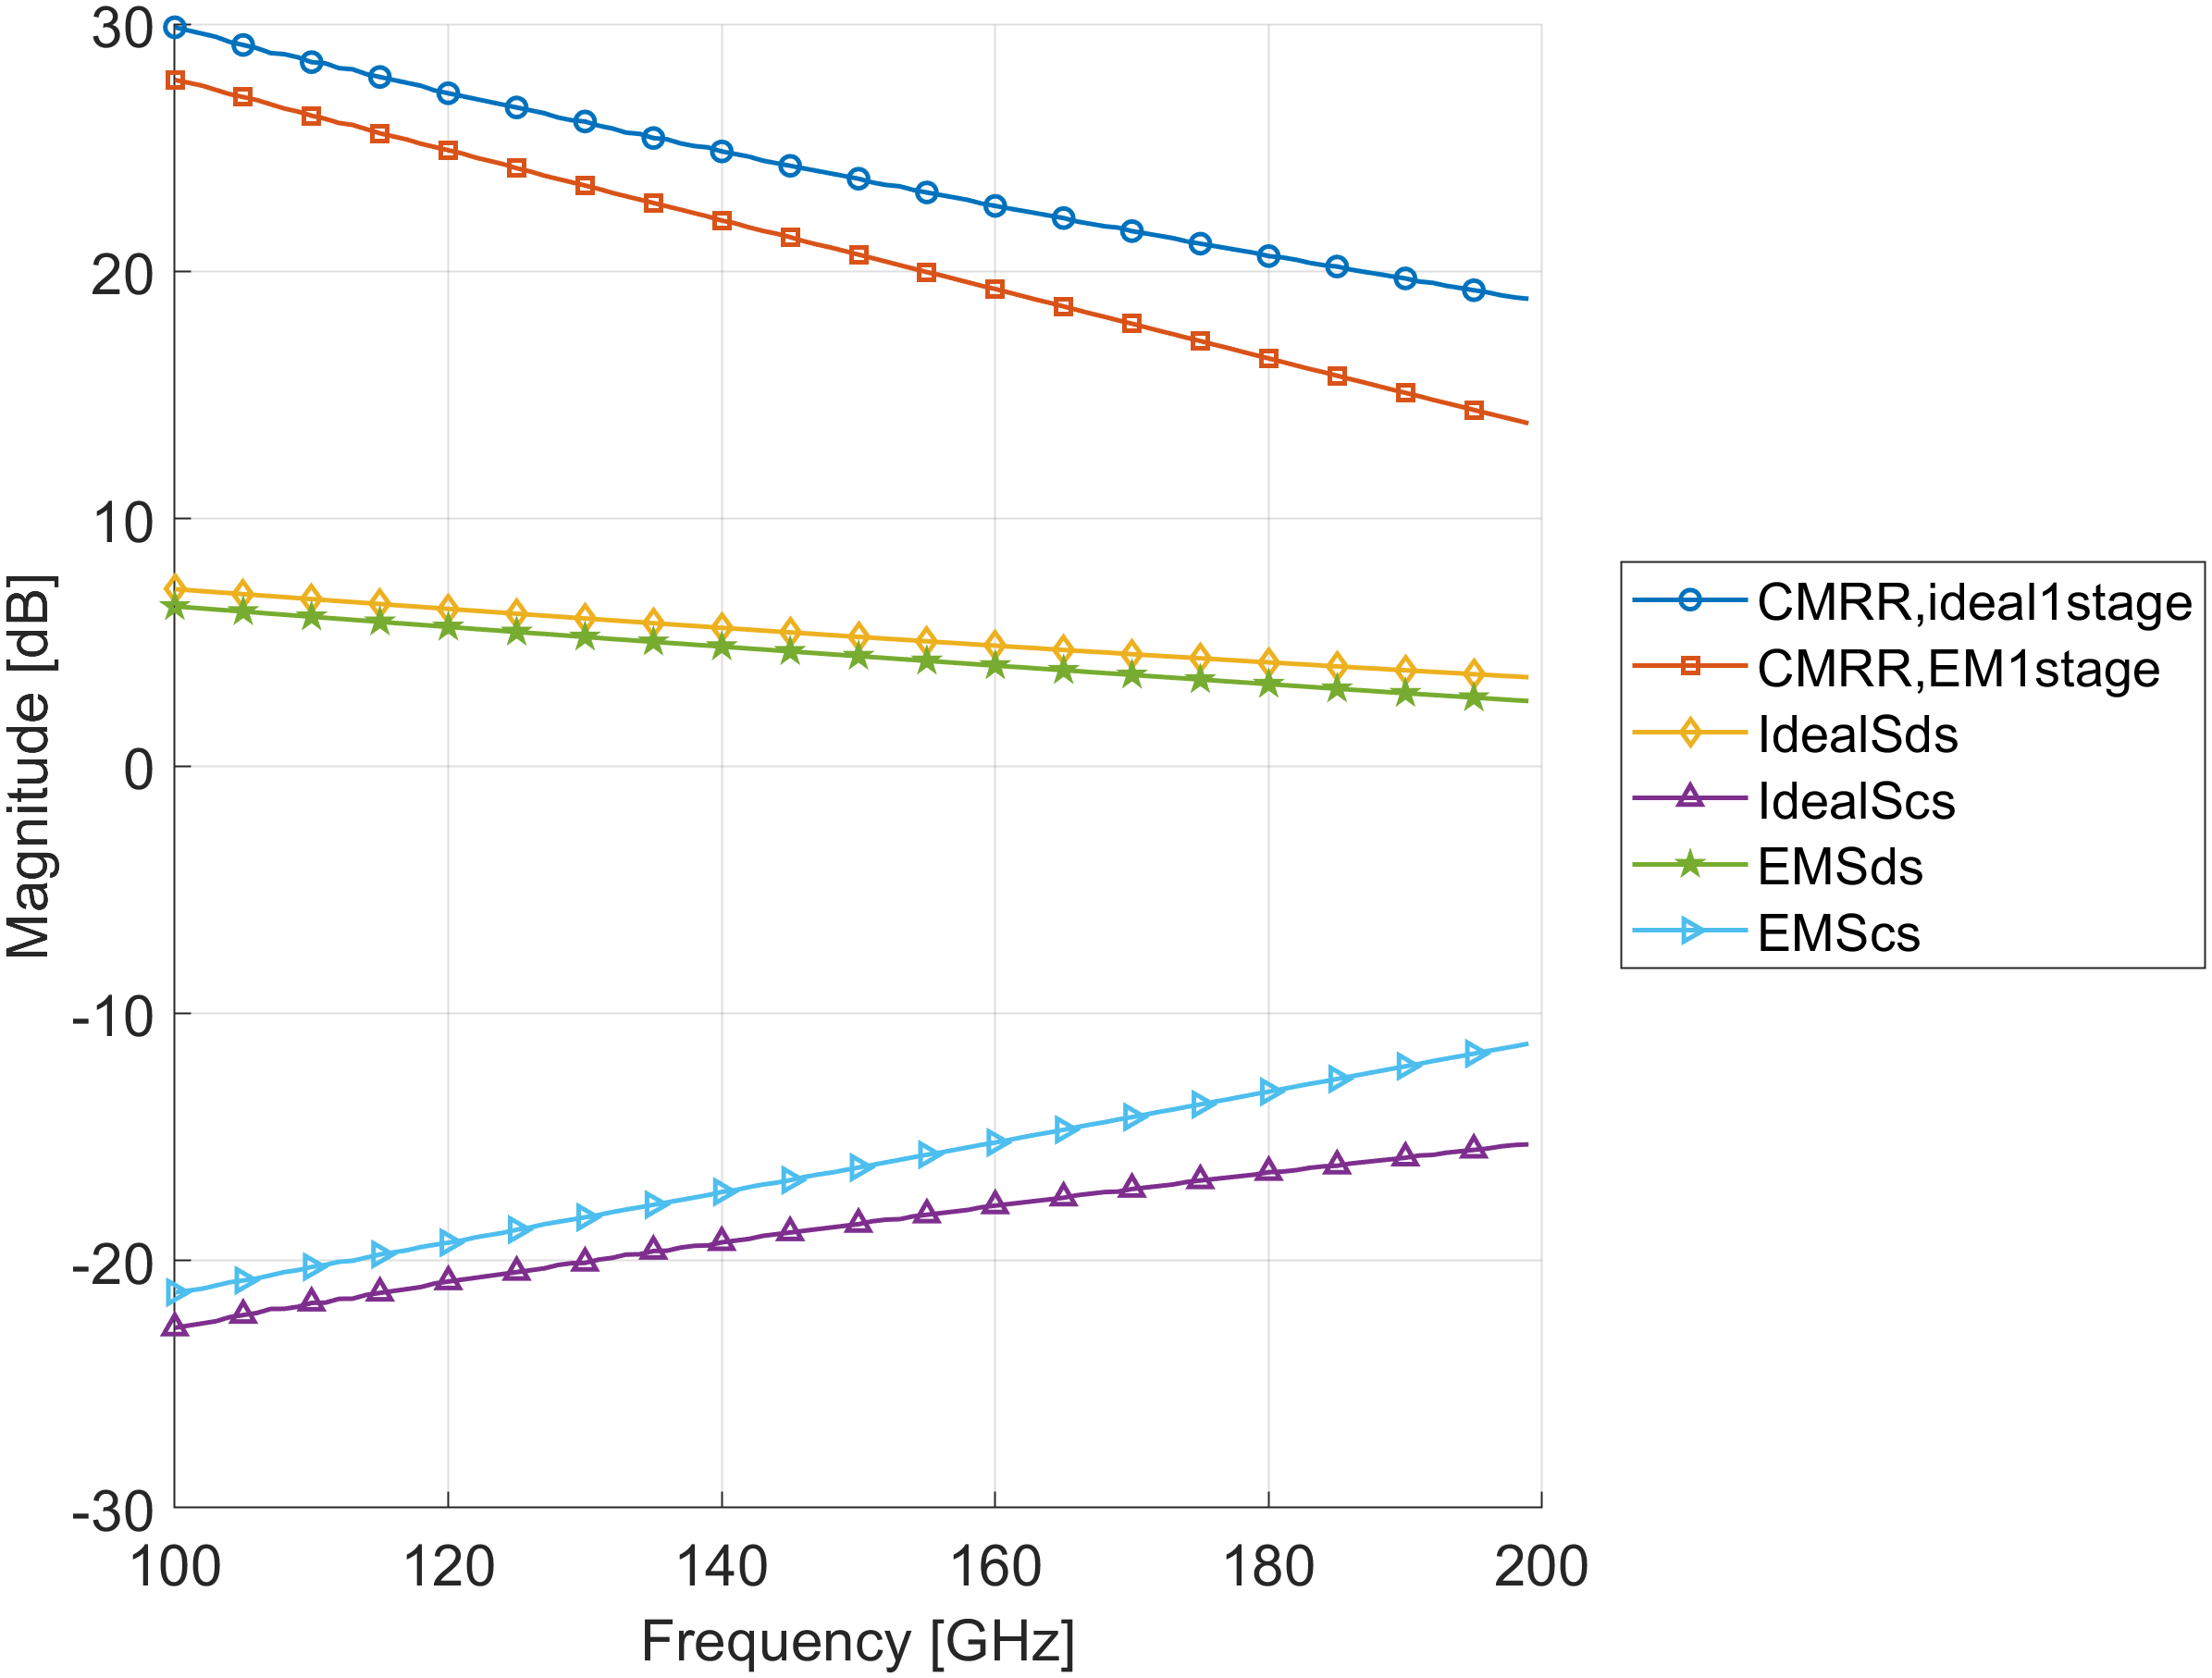
\includegraphics[width=0.7\linewidth]{Design_figures/Layout/ComparisonMeasurements/MixedPardB_CMRRComparisons1Stage_Ideal_EM.png}
    \caption{Simulation and comparison for CMRR, the single to differential S parameter ($\mathrm{S}_\mathrm{ds}$) and the single to common S parameter($\mathrm{S}_\mathrm{cs}$) for the ideal and EM first stage balun.}
    \label{fig:MixedPardB_CMRRComparisons1Stage_Ideal_EM}
\end{figure}

\begin{figure}[hbt!]
    \centering
    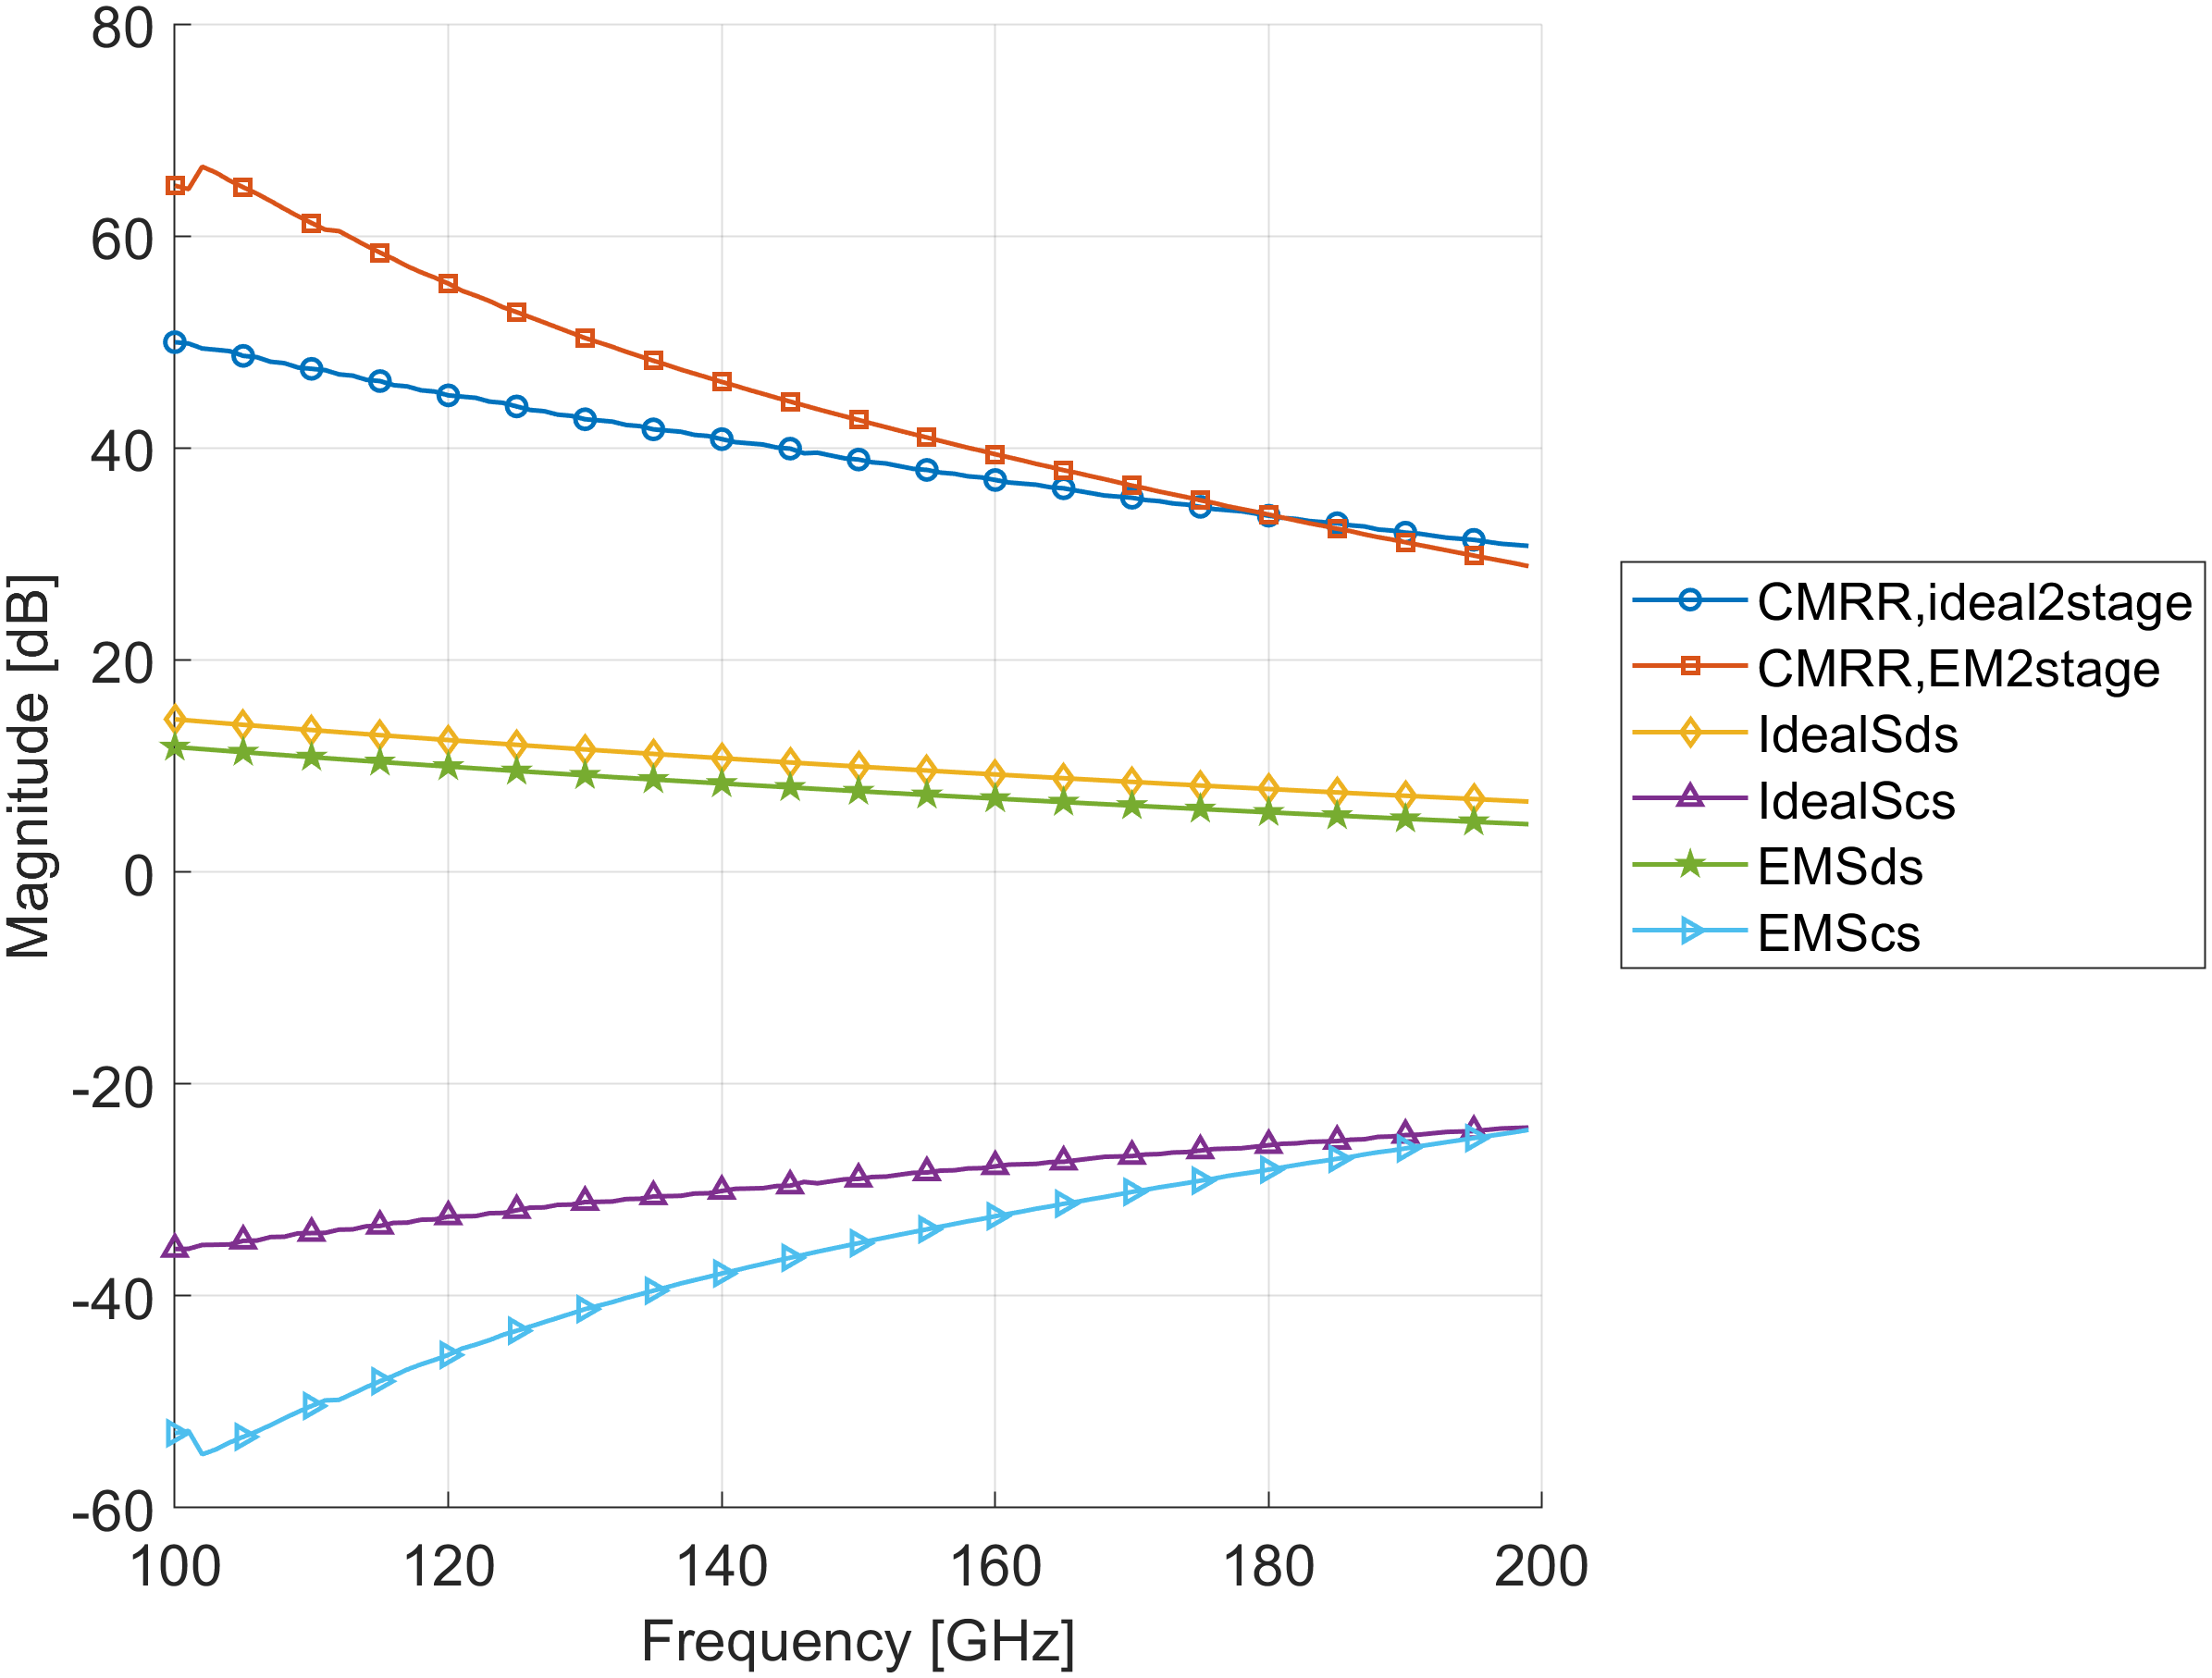
\includegraphics[width=0.7\linewidth]{Design_figures/Layout/ComparisonMeasurements/MixedPardB_CMRRComparisons2Stage_Ideal_EM.png}
    \caption{Simulation and comparison for CMRR, the single to differential S parameter ($\mathrm{S}_\mathrm{ds}$) and the single to common S parameter($\mathrm{S}_\mathrm{cs}$) for the ideal and EM "two-stage" balun.}
    \label{fig:MixedPardB_CMRRComparisons2Stage_Ideal_EM}
\end{figure}

\cleardoublepage
\paragraph{Power gain of the three-stage design with EM cores} It is useful to carry out a retrospective analysis from this point to compare it with the results obtained with the matching network used in the layout design, section \ref{sec:Layout_Design}.
The overall design can be thought as an unilateral two port network, presented as a black box capable of a forward transmission gain $\mathrm{S}_{21}$ and a reverse transmission gain $\mathrm{S}_{12}$ given in Figure \ref{fig:ConnectedCoresNoMN_ExtractPar_S_MaxGain_GSmax_G0_GLmax_GTmax}. Based on the results obtained from the interstage matching network, this black box effectively represents the overall design configuration and can be used to compare the actual results in section \ref{sec:Simulations_And_Discutions}.
The maximum unilateral transducer power gain of a two port network is achieved by applying simultaneous conjugated matching networks at the input and output ports \cite{Microwave Transistor Amplifiers Analysis and Design}.
The maximum input ($G_{S\mathrm{max}}$) and output contributions achievable ($G_{L\mathrm{max}}$), according to \eqref{eq:GutMax}, are between \SI{1.7}{\decibel} and \SI{3}{\decibel} over the D-band.\\
These data suggest that designing input and output networks to create conjugate impedances is useful to increase the gain by almost \SI{4.7}{\decibel}. Furthermore, broadband input and output matching networks are important to connect the device to the external world, reducing reflection losses and therefore improving the available power at the input and at the output of the network.

\begin{figure}[hbt!]
    \centering
    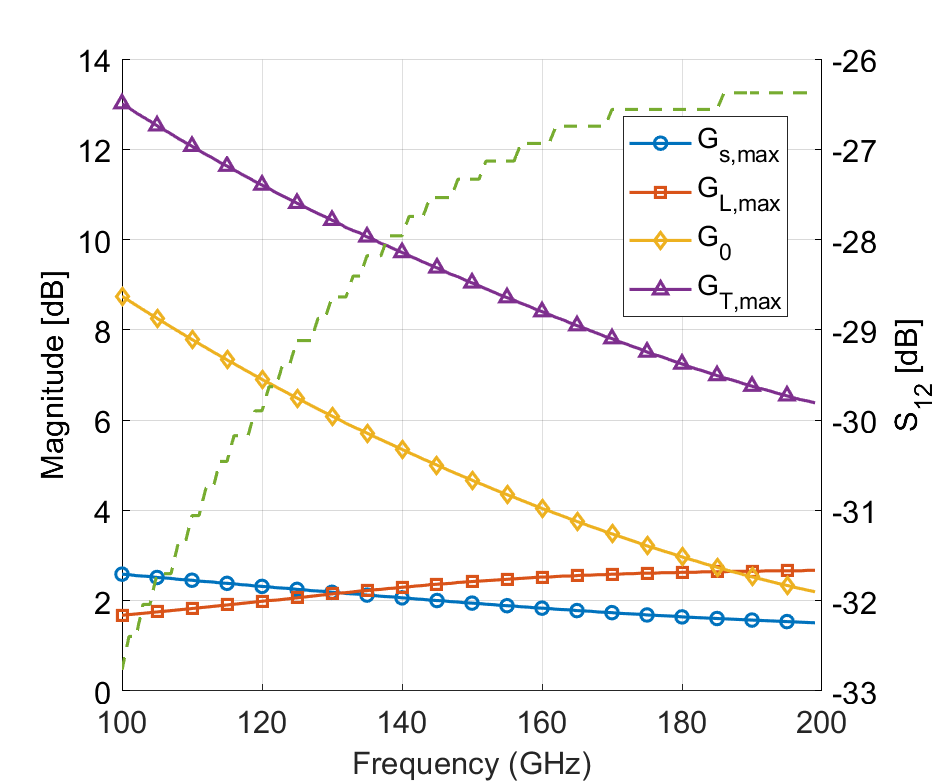
\includegraphics[width=0.65\linewidth]{Design_figures/Layout/Layout3StageMerged_noMNMeasurements/EMDiffBalun_EMDiffAmplifier_EMCBAmplifier_ConnectedCoresNoMN_ExtractPar_S_MaxGain_GSmax_G0_GLmax_GTmax.png}
    \caption{Simulations of $G_{S\mathrm{max}}$, $G_0$, $G_{L\mathrm{max}}$, $G_{T\mathrm{max}}$, and $S_{12}$ of the Three-Stage with EM cores and without matching networks.}
    \label{fig:ConnectedCoresNoMN_ExtractPar_S_MaxGain_GSmax_G0_GLmax_GTmax}
\end{figure}


\cleardoublepage
\subsection{Final layout-schematic}
\label{Analysis_combined_core}
The design shown in Figure \ref{fig:Schematic_of_design_simulation_before_the_tapeout} has been submitted for the tapeout after the biasing networks and the fillers were applied and it is, essentially, the last simulation-level design done for this design.

\begin{figure}[hbt!]
    \centering
    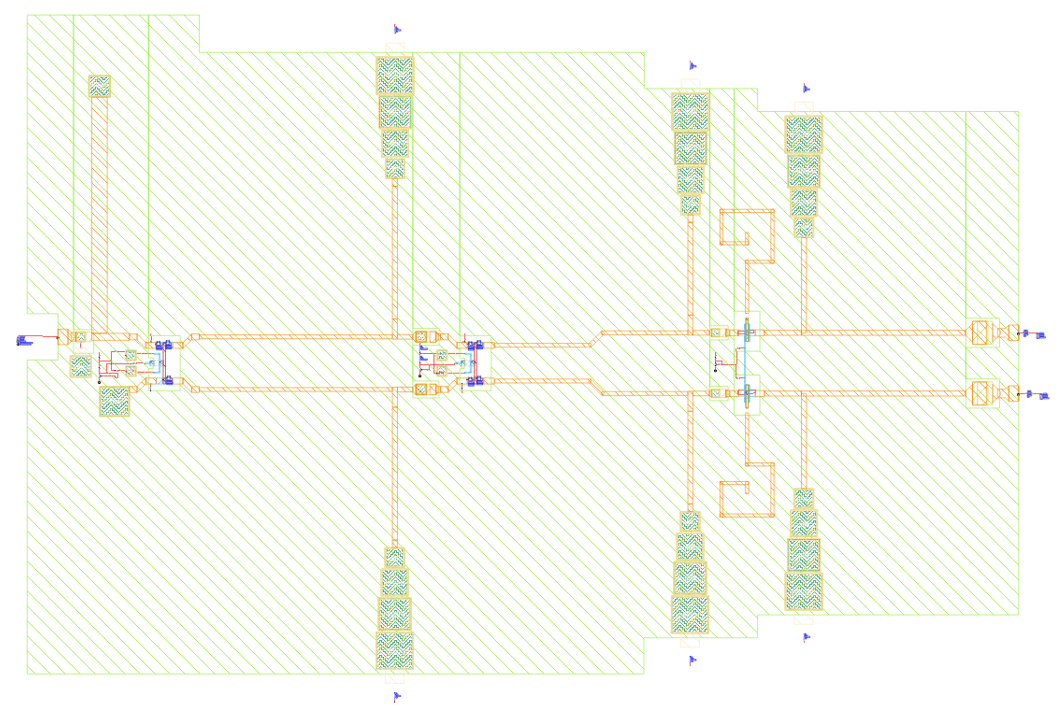
\includegraphics[width=1\linewidth]{Design_figures/Layout/TapeoutSchematics/SchematicTapeout.png}
    \caption{Schematic of the designed layout simulation before tapeout.}
    \label{fig:Schematic_of_design_simulation_before_the_tapeout}
\end{figure}

The plots in this part are omitted as they are presented in Section \ref{sec:Simulations_And_Discutions}.

%%%%%%%%%%%%%%%%%%%%%%%%%%%%%%%%%%%%%%%%%%%%%%%%%%%%%%%%%%%%%%%%%%%
%
\cleardoublepage
\subsection{Layout-level design}
%
\begin{figure}[hbt!]
    \centering
    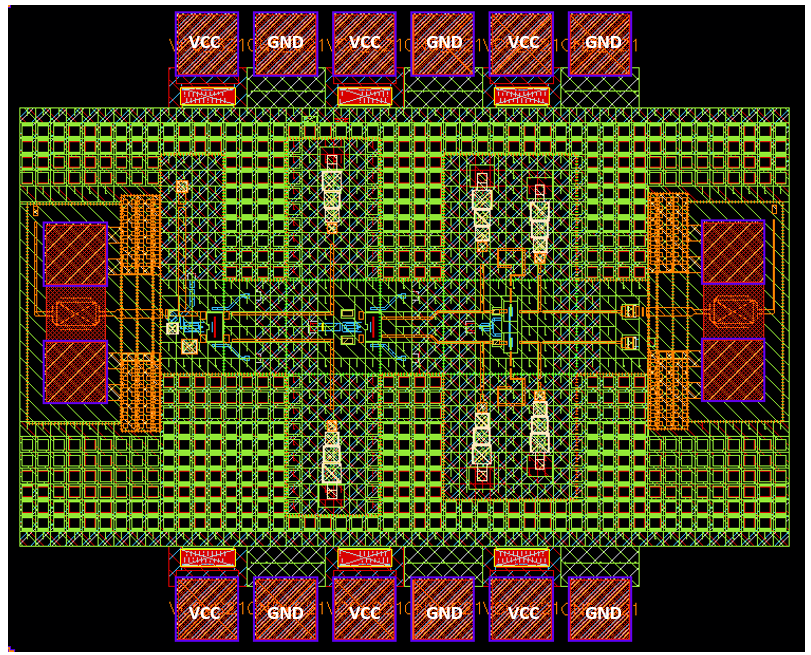
\includegraphics[width=1\linewidth]{Design_figures/Layout/LayoutCompleteS21.png}
    \caption{Layout of the balun submitted for tapeout. This figure shows the balun with the top-right output port ($S_{21}$), while the bottom output port ($S_{31}$) is terminated with an EM \SI{50}{\ohm} load.}
    \label{fig:LayoutCompleteS21}
\end{figure}
The final layout with fillers is shown in Figure~\ref{fig:LayoutCompleteS21}.
Through the use of RF probes in GSG configuration, the RF input signal is applied on the left side and the output signal is taken from one of the output ports on the right side, while the other is terminated with a \SI{50}{\ohm} load within the layout.
A second circuit with inverted output ports was also designed and is shown in the chip overview in Appendix~\ref{sec:Appendix}, Figure~\ref{fig:TapeoutChip}.

The upper and lower pads are needed to provide the supply voltage and ground through their respective probes. Furthermore, there are no biasing pads that would allow connection to external sources, since the biasing network is integrated internally. This ensures that the design works as analyzed in the previous sections, although it also limits its flexibility due to the absence of bias-voltage tuning in case it is needed.

\newpage
\subsection{Biasing networks}
\begin{figure}[hbt!]
    \centering
    % --- Figura (a) ---
    \begin{subfigure}{0.45\textwidth}
        \centering
        \begin{circuitikz}[scale=0.8, transform shape]
            \draw (0,0) node[npn, xscale=-1, anchor=B] (npn1) {\ctikzflipx{$Q11(Q12)$}};
            \draw (npn1.B) to [R,l=${R_{11}(R_{14})}$,a=\SI{4}{\kohm}]++(0.75,0)--++(0.45,0) coordinate (x) --++(0.45,0) to [short,-o]++(0.45,0)node[right]{$V_{B1}=0.92V$};
            \draw (npn1.C)--++(0,0.25) coordinate(cx);
            \draw (x) to [short,*-]++(0,1)-|(cx) to [short,-*]++(0,0) to [R,l=${R_{12}(R_{15})}$,a=\SI{175}{\ohm}]++(0,1.5) --++(0,0.15) coordinate(vb1);
            \draw(vb1) to [R,l=${R_{13}(R_{16})}$,a=\SI{205}{\ohm}]++(0,1) --++(0,0.15) coordinate(vcc);
            \draw (vb1)--++(0,-0.2) to [short,*-o]++(1.45,0)node[right]{$V_{B2}=1.33V$};
            \draw (vcc) --++(0,0.1) to [open]++(-0.5,0) --  node[anchor=south] {$\mathrm{V}_\mathrm{CC}$} ++(1,0);
            \draw(npn1.E)--++(0,-0.05) node[ground]{};
            %current
            \draw[-latex](-1.25,2.85)--++(0,-0.825) node[anchor=south east ]{2.32mA};
        \end{circuitikz}
        \caption{}
         \label{fig:Schematic_Biasig_First&SecondStage}
    \end{subfigure}
    \hfill
    % --- Figura (b) ---
    \begin{subfigure}{0.45\textwidth}
        \centering
        \begin{circuitikz}[scale=0.8, transform shape]
            \draw (0,0) node[npn, xscale=-1, anchor=B] (npn1) {\ctikzflipx{$Q13$}};
            \draw (npn1.B) to [R,l=$R_{17}$,a=\SI{4}{\kohm}]++(0.75,0)--++(0.45,0) coordinate (x) --++(0.45,0) to [short,-*]++(0.45,0) coordinate(ouo);
            \draw(ouo)--++(0,0.75)to[short,-o]++(0.5,0)node[right]{$V_{B}=0.9$V};
            \draw(ouo)--++(0,-0.75)to[short,-o]++(0.5,0)node[right]{$V_{B}=0.9$V};
            \draw (npn1.C)to[short,-*]++(0,0.25) coordinate(cx);
            \draw (x) to[short,*-] ++(0,1) -| (cx) to[R,l=$R_{18}$,a=\SI{340}{\ohm}] ++(0,1.75) -- ++(0,0.4) coordinate(vcc);
            \draw (vcc) to [open]++(-0.5,0) --  node[anchor=south] {$\mathrm{V}_\mathrm{CC}$} ++(1,0);
            \draw(npn1.E)--++(0,-0.05) node[ground]{};
            %current
            \draw[-latex](-1.25,3)--++(0,-0.825) node[anchor=south east ]{\SI{2.26}{\milli\ampere}};
        \end{circuitikz}
        \caption{}
        \label{fig:Schematic_Biasig_ThirdStage}
    \end{subfigure}
    \caption{Schematic of the biasing networks: (a) first and second stage biasing network; (b) third stage biasing network.}
    \label{fig:Schematic_Biasig}
\end{figure}


The biasing networks are based on the "resistor ratioed current mirror" theory \cite{A 2.4 GHz SiGe HBT high voltage high power amplifier}\cite{High power density SiGe millimeter-wave power amplifiers}\cite{ShresthaAmit} although it isn't applied in the final layout of the last stage. 

The biasing side of the current mirror in the first two stages is schematically identical, as shown in Figure~\ref{fig:Schematic_Biasig_First&SecondStage}, and presents a area ratio of 2:1 between Q4(Q8) and Q11(Q12). By sizing the resistors ratio to 2, it is possible to relate the current ratio only to the resistors. This provides a stable biasing point in temperature compared to a non ratioed current mirror. Also, these two current mirrors incorporate an additional voltage divider to bias the bases Q3 and Q7.\\ 
Their symmetrical layout are shown in Figure~\ref{fig:Layout_of_the_biasing_network_of_the_first_stage} and Figure~\ref{fig:Layout_of_the_biasing_network_of_the_second_stage}.
\begin{figure}[hbt!]
    \centering
        \begin{overpic}[width=0.7\linewidth]{Design_figures/Layout/BiasingLayoutFirstStage.png}
        
        \put(52,44){\scriptsize \textcolor{white}{Q1}}
        \put(52,21){\scriptsize \textcolor{white}{Q2}}
        \put(51,30){\scriptsize \textcolor{white}{Q3}}
        \put(43,30){\scriptsize \textcolor{white}{Q4}}
        \put(25,30){\scriptsize \textcolor{white}{Q11}}
        
        \put(44.5,44){\scriptsize \textcolor{white}{R1}}
        \put(44.5,21){\scriptsize \textcolor{white}{R2}}
        \put(40,39){\scriptsize \textcolor{white}{2*R3}}
        \put(40,27){\scriptsize \textcolor{white}{2*R3}}
        \put(38,34.5){\scriptsize \textcolor{white}{R4}}
        \put(30.35,34.5){\scriptsize \textcolor{white}{R11}}
        \put(21.25,35.5){\scriptsize \textcolor{white}{R12}}
        \put(15.5,33){\scriptsize \textcolor{white}{R13}}

        \put(26.5,73){\scriptsize \textcolor{white}{VCC}}
        \put(80,61){\scriptsize \textcolor{white}{VCC}}
        \put(80,5){\scriptsize \textcolor{white}{VCC}}
        
    \end{overpic}
    \caption{Layout of the biasing network of the first stage}
    \label{fig:Layout_of_the_biasing_network_of_the_first_stage}
\end{figure}
\\The biasing of the transistors Q1(Q5), Q2(Q6), Q3(Q7) and Q4(Q8) consists of a \SI{2}{\kilo\ohm} series resistor connecting their bases to Vcc. These connections are made in the same way for each transistor, as follows: the routing starts from the base of the transistor in Metal1, then goes to the Metal1-to-TopMetal2 via, which is used to connect the core to the input network. The corresponding \SI{2}{\kohm} resistor ($\mathrm{R}_1$,$\mathrm{R}_2$,$\mathrm{R}_5$,$\mathrm{R}_6$) is connected to one edge of this via and an additional routing in Metal 1 is used to reach the supply layer in Metal3, ending with a via connection between the two metals. Along this last path, the Metal1 widths are increased as soon as possible to reduce the parasitic resistance.
\begin{figure}[hbt!]
    \centering
        \begin{overpic}[width=0.7\linewidth]
        {Design_figures/Layout/BiasingLayoutSecondStageV2.png}
        
        \put(58.5,56){\scriptsize \textcolor{white}{Q5}}
        \put(58.5,31){\scriptsize \textcolor{white}{Q6}}
        \put(62,43){\scriptsize \textcolor{white}{Q7}}
        \put(49,41){\scriptsize \textcolor{white}{Q8}}
        \put(35.5,40){\scriptsize \textcolor{white}{Q12}}
        
        \put(53,54.5){\scriptsize \textcolor{white}{R5}}
        \put(53,32){\scriptsize \textcolor{white}{R6}}
        \put(49,49){\scriptsize \textcolor{white}{2*R7}}
        \put(49,37){\scriptsize \textcolor{white}{2*R7}}
        \put(43.5,47){\tiny \textcolor{white}{$\dfrac{C_1}{2}$}}
        \put(43.5,40){\tiny \textcolor{white}{$\dfrac{C_1}{2}$}}
        \put(49,44){\scriptsize \textcolor{white}{R8}}
        \put(40,44){\scriptsize \textcolor{white}{R14}}
        \put(33,45.5){\scriptsize \textcolor{white}{\rotatebox{90}{R15}}}
        \put(29,41.5){\scriptsize \textcolor{white}{\rotatebox{90}{R16}}}

        \put(5,43){\scriptsize \textcolor{white}{VCC}}
        
    \end{overpic}
    \caption{Layout of the biasing network of the second stage. The routing of the bases of Q5 and Q6 is not shown in this figure, but it is the same as in the first stage.}
    \label{fig:Layout_of_the_biasing_network_of_the_second_stage}
\end{figure}
\\

The biasing of the third stage consists of a \SI{2}{\kohm} series resistor connected to the remaining part of the current mirror in Figure~\ref{fig:Schematic_Biasig_ThirdStage}. Unlike in the previous stages, the current mirror is designed with a 6:1 ratio with Q13, meaning that the base resistor $\mathrm{R}_{17}$ should also have been six times larger than $\mathrm{R}_{10}$ and $\mathrm{R}_{9}$. 
\begin{comment}
furthermore, by using this symmetrical structure, the total resistance seen from the biasing input to the amplifier is \SI{4}{\kohm}, and the ideal base resistor value required to achieve thermal stability should have been \SI{32}{\kohm}. 
\end{comment}
Since this value was impractical to implement in this design due to the size required within the layout area, the resistors were chosen to be equal and therefore the ratioed current mirror was not applied.
An alternative solution was to bias each CB amplifier with an independent current mirror. This approach was not adopted because possible asymmetries in the implementation could degrade the balance performance.\\
The layout realization of the third stage biasing network is shown in Figure~\ref{fig:Layout_of_the_biasing_network_of_the_third_stage}.\\
\begin{figure}[hbt!]
    \centering
    \begin{overpic}[width=0.85\linewidth]
    {Design_figures/Layout/BiasingLayoutThirdStage.png}
        
        \put(63,44){\footnotesize \textcolor{white}{Q9}}
        \put(63,20){\footnotesize \textcolor{white}{Q10}}
        \put(20.5,37){\footnotesize \textcolor{white}{Q13}}

        \put(61.5,61){\footnotesize \textcolor{white}{L1}}
        \put(61.5,2){\footnotesize \textcolor{white}{L2}}
        
        \put(51,43){\footnotesize \textcolor{white}{R9}}
        \put(50.5,24){\footnotesize \textcolor{white}{R10}}
        \put(28,30){\footnotesize \textcolor{white}{R17}}
        \put(14.5,34.5){\footnotesize \textcolor{white}{R18}}

        \put(6.5,31.5){\footnotesize \textcolor{white}{VCC}}
        
    \end{overpic}
    \caption{Layout of the biasing network of the third stage}
    \label{fig:Layout_of_the_biasing_network_of_the_third_stage}
\end{figure}\\
The routing consists of a resistor connecting the base of the transistor in Metal1 to the common connection of the diode-connected BJT. Another resistor is placed between this node and the base of transistor Q13. The collector is connected directly to the Metal3 supply layer through resistor $\mathrm{R}_{18}$ and a Metal1-to-Metal3 via.

%%%%%%%%%%%%%%%%%%%%%%%%%%%%%%%%%%%%%%%%%%%%%%%%%%%%%%%%%%%%%%%%%%%
\cleardoublepage
\subsection{Matching networks}

This section presents the layout of the matching networks, focusing on the topological aspect and the choices made for the arrangement of the components.\\
The following plots, where possible, are extrapolated from the CSV files of the ADS keysight "SP\_Probes" tool, utilized in the schematic in Figure \ref{fig:Schematic_of_design_simulation_before_the_tapeout}. Therefore, the simulations do not represent the results achieved by the independent networks as they are shown, but rater as the overall result obtained from the interaction of multiple factors within the EM design.

\paragraph{Input matching network}\mbox{}\\
The input matching network was designed and realized making sure that the reflection coefficient stays near or under \SI{-10}{\decibel} along the bandwidth.
The layout consist, looking from the left to the right, by a series capacitor, a shunt impedance made by a resist and a capacitor connected to ground, a short stub and a transmission line.
\begin{figure}[hbt!]
    \centering
    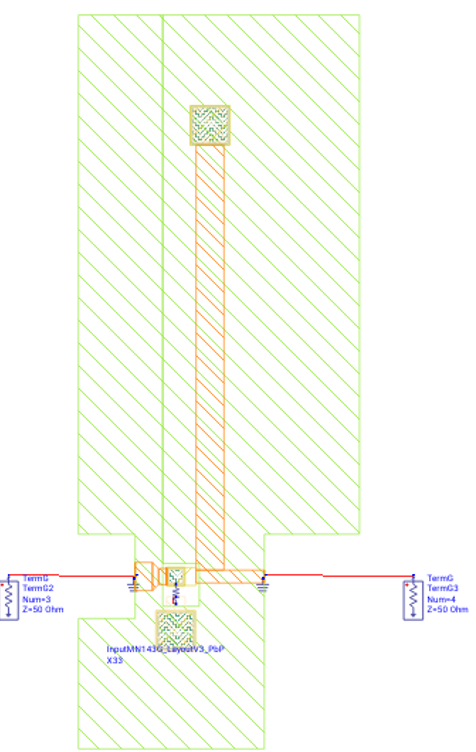
\includegraphics[width=0.5\linewidth]{Design_figures/Layout/MatchingNetworks/LayoutInputMN.png}
    \caption{Layout of the input matching network}
    \label{fig:placeholder}
\end{figure}
\begin{center}
\begin{figure}[H]
    \centering
    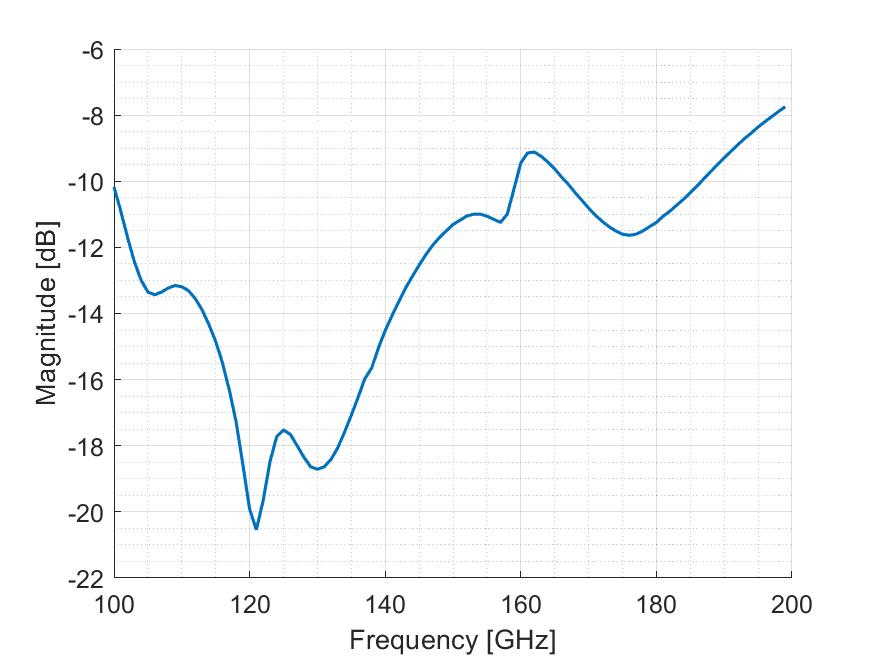
\includegraphics[width=0.5\linewidth]{Design_figures/Layout/MeasurementsMN_SPprobes/MeasurementMN_S11_Mag.png}
    \caption{Simulation results for the input stage matching network}
    \label{fig:placehMeasurementMN_S11_Magolder}
\end{figure}
\end{center}

\paragraph{Interstage matching networks}\mbox{}\\
 The interstage impedances were matched using differential terminations between stages to extract the differential output impedance of the first stage and the differential input impedance of the second stage. This enabled the design of a symmetric topology, adopted for both interstages, consisting of a long transmission line, a short stub, and a series capacitor.  
 However this topology provides limited flexibility for broadband matching and thus represents the weak point of the overall matching. \\
 The first interstage matching network is shown at the center of Figure~\ref{fig:one_interstages} , while the magnitudes[dB] of the S parameters extracted from the CSV files are shown on the sides, for the input and output, respectively. The output ports show a narrowband behavior with a peak at \SI{182}{\giga\hertz}, with the top branch performing relatively better than the bottom one.
This network does not provide good matching, but it still performs far better than the one used for the second interstage, whose circuit is shown in Figure~\ref{fig:two_interstages}.\\
 The second interstage uses the same network topology as the first one, but the S parameters struggle to go below \SI{-5}{\decibel} over the whole frequency range for both the input and output ports. This degradation is due to the change of the input impedance after the removal of the third-stage capacitance, Figure ~\ref{fig:SmithPlot_AllSweeps_ComparisonText}.

\begin{landscape}
\centering
\begin{figure}
% ====== First interstage row ======
\begin{tabular}{ m{0.35\linewidth} m{0.2\linewidth} m{0.35\linewidth} }
    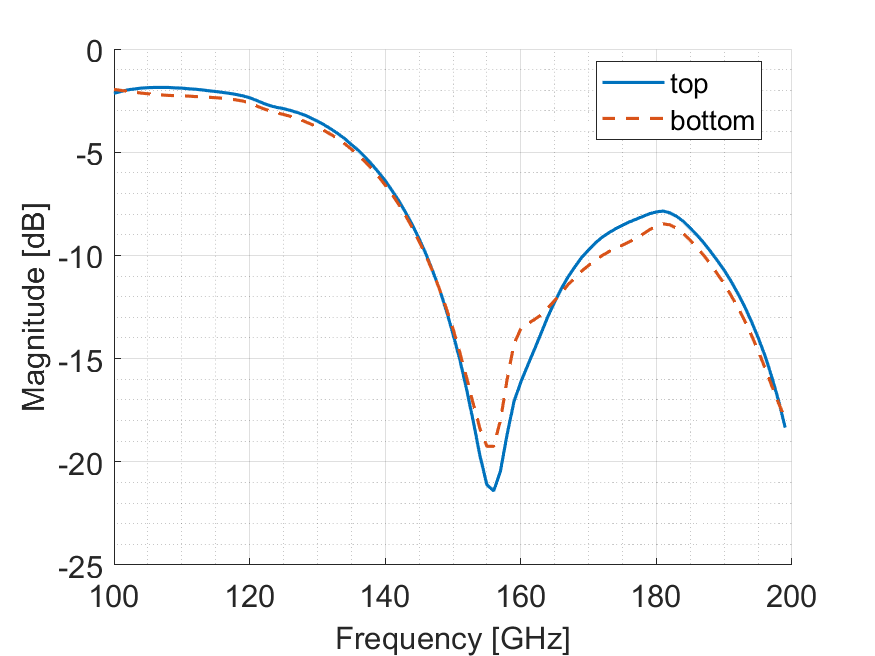
\includegraphics[width=\linewidth]{Design_figures/Layout/MeasurementsMN_SPprobes/MeasurementMN_SProbe2&3R_Mag.png} &
    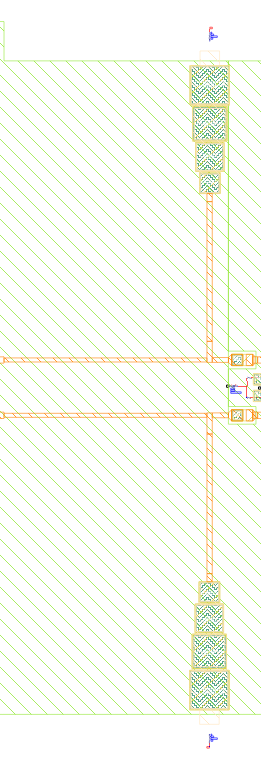
\includegraphics[width=\linewidth]{Design_figures/Layout/MatchingNetworks/LayoutFirstInterstageMN.png} &
    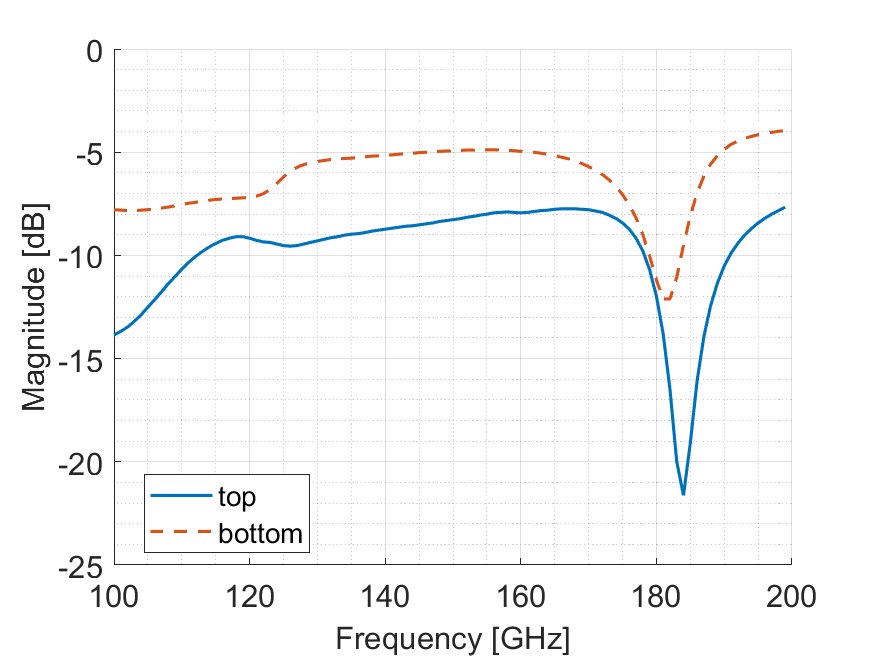
\includegraphics[width=\linewidth]{Design_figures/Layout/MeasurementsMN_SPprobes/MeasurementMN_SProbe4&5L_Mag.png} \\
\end{tabular}
\caption{Layout and simulation results of the first interstage matching network. The simulation results are shown alongside the corresponding Port.}
\label{fig:one_interstages}
\end{figure}
\end{landscape}


\begin{landscape}
\begin{figure}
\centering
% ====== Second interstage row ======
\begin{tabular}{ m{0.35\linewidth} m{0.28\linewidth} m{0.35\linewidth} }
    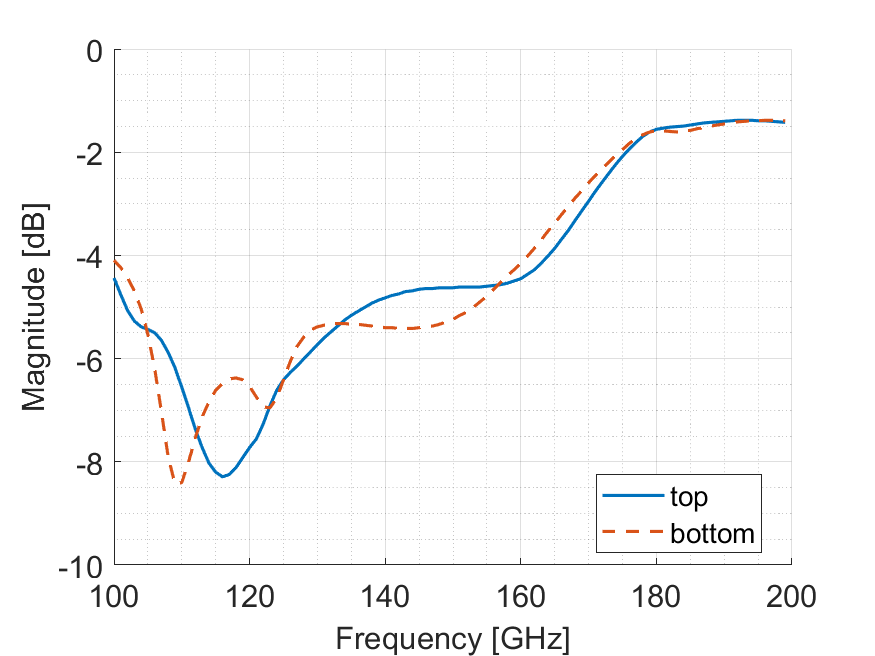
\includegraphics[width=\linewidth]{Design_figures/Layout/MeasurementsMN_SPprobes/MeasurementMN_SProbe6&7R_Mag.png} &
    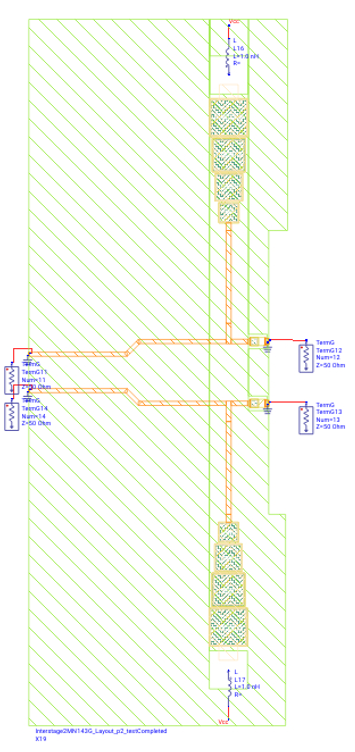
\includegraphics[width=\linewidth]{Design_figures/Layout/MatchingNetworks/LayoutSecondInterstageMN.png} &
    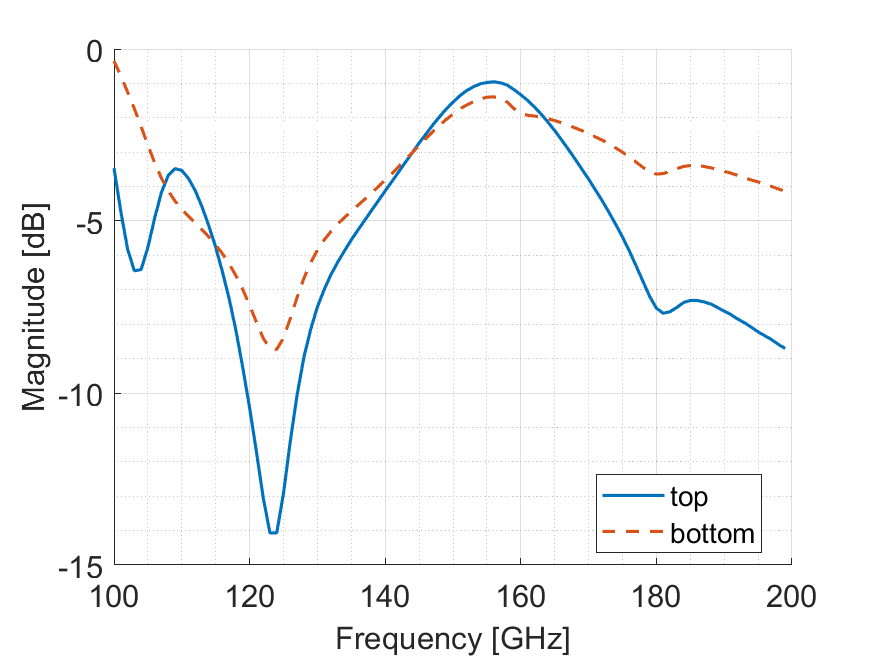
\includegraphics[width=\linewidth]{Design_figures/Layout/MeasurementsMN_SPprobes/MeasurementMN_SProbe8&9L_Mag.png} \\
\end{tabular}
\caption{Layout and simulation results of the second interstage matching network. The simulation results are shown alongside the corresponding Port.}
\label{fig:two_interstages}
\end{figure}
\end{landscape}

\newpage
\paragraph{Output matching network}\mbox{}\\
For the latter stage, after the changes described in Section~\ref{subsubsec:Layout of the third stage}, the adopted configuration consists of a line, a short stub, another line, and a MOM capacitor.
Also, unlike the previous networks, the S parameters of the output were imported within the ADS Smith Chart tool (Figure \ref{fig:matchingOutput}), allowing to foresee the variation of load impedance over frequency and therefore, reducing the mismatch that would otherwise have occurred in the case of a wideband matching network based on an fixed impedance value extracted at a single frequency.
\begin{figure}[hbt!]
    \centering
    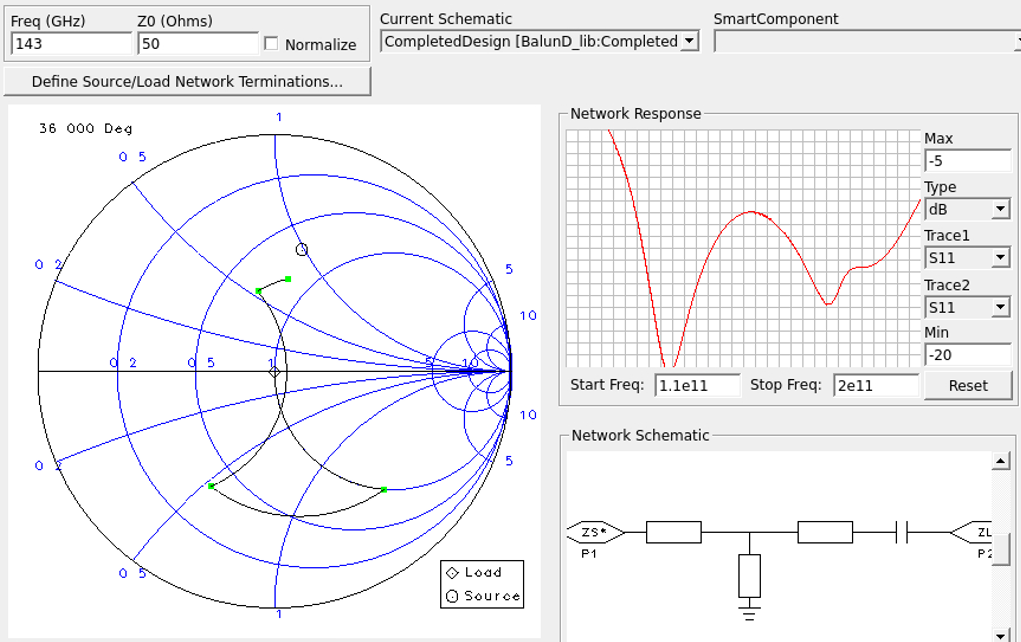
\includegraphics[width=0.75\linewidth]{Design_figures/matchingOutput.png}
    \caption{Preview of the ideal output stage matching network in the ADS Smith Chart Tool.}
    \label{fig:matchingOutput}
\end{figure}\\
 The results of the output ports are identified as $\mathrm{S}_{22}$ and $\mathrm{S}_{33}$ shown in the next figure.
\begin{figure}[!hbt]
    \centering
    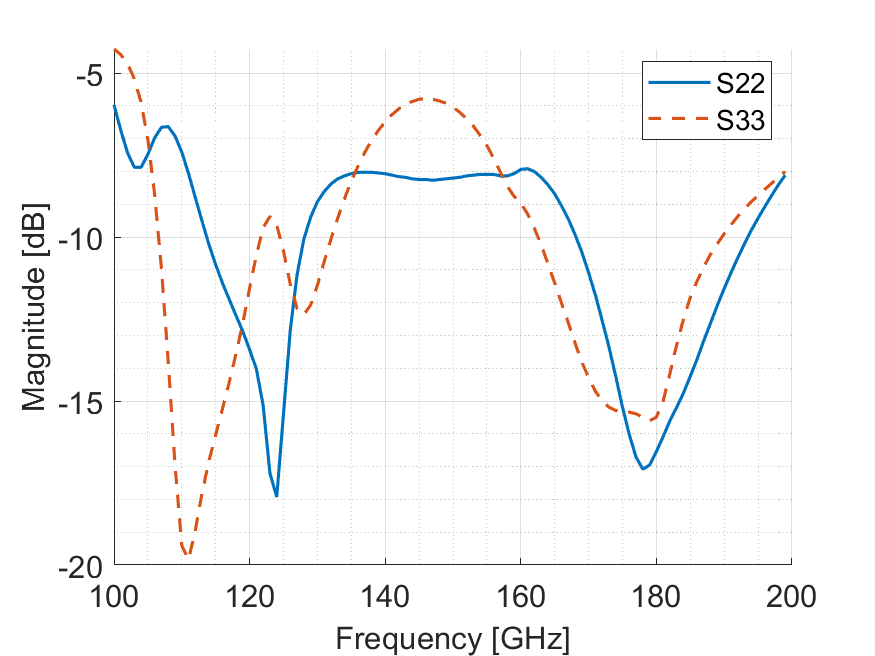
\includegraphics[width=0.5\linewidth]{Design_figures/Layout/MeasurementsMN_SPprobes/MeasurementMN_S22&S33_Mag.png}
    \caption{Simulated forward transmission gain at the top ($\mathrm{S}_{21}$) and bottom ($\mathrm{S}_{31}$) output ports with ideal \SI{50}{\ohm} loads.}
    \label{fig:placeholder}
\end{figure}\\
A picture of this network its not present from a closed view, but it still can be seen in the complete circuit in Figure \ref{fig:Schematic_of_design_simulation_before_the_tapeout} and Figure \ref{fig:LayoutCompleteS21}.